% latex_includes.tex —— 22 张 DATA 图的 LaTeX 插图块（由 figures/gen_fig_*.py 真算生成）
% 用法：在 main.tex 导言区确保已载入 graphicx + float，然后 % latex_includes.tex —— 22 张 DATA 图的 LaTeX 插图块（由 figures/gen_fig_*.py 真算生成）
% 用法：在 main.tex 导言区确保已载入 graphicx + float，然后 % latex_includes.tex —— 22 张 DATA 图的 LaTeX 插图块（由 figures/gen_fig_*.py 真算生成）
% 用法：在 main.tex 导言区确保已载入 graphicx + float，然后 % latex_includes.tex —— 22 张 DATA 图的 LaTeX 插图块（由 figures/gen_fig_*.py 真算生成）
% 用法：在 main.tex 导言区确保已载入 graphicx + float，然后 \input{figures/latex_includes}
%       或按需把下面单个 figure 环境复制到对应章节。
% 说明：全部为矢量 PDF，插入宽度统一 0.90\textwidth（各图长宽比同属一档）。
%       图内只保留必要数值与短锚点，口径/结论一律写在下方 caption 里。

\begin{figure}[H]
  \centering
  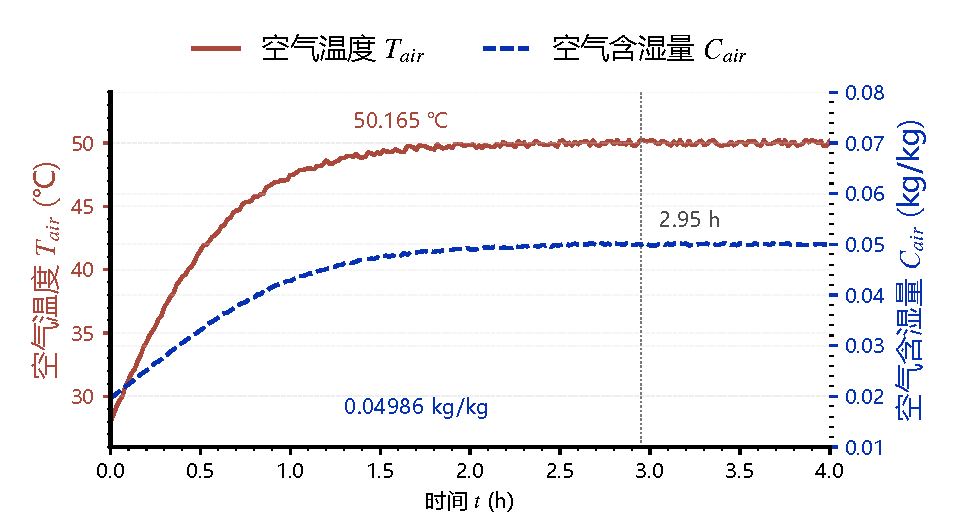
\includegraphics[width=0.9\textwidth,height=0.8\textheight,keepaspectratio]{figures/fig_input_chamber.pdf}
  \caption{附件 1 干燥室工况的双轴时程。左轴为空气温度 $T_{air}(t)$，右轴为空气含湿量
  $C_{air}(t)$。温度自 $28~^\circ$C 快速抬升，$1.37$~h 已达 $49~^\circ$C，
  峰值 $50.246~^\circ$C 出现在 $2.95$~h，随后进入平台段；含湿量峰值 $0.05025$~kg/kg。
  该平台值即问题 2--4 长时程求解所用的边界驱动。两轴量程刻意错开，使两族曲线各占一个
  纵向带，避免读图时混淆归属。}
  \label{fig:input_chamber}
\end{figure}

\begin{figure}[H]
  \centering
  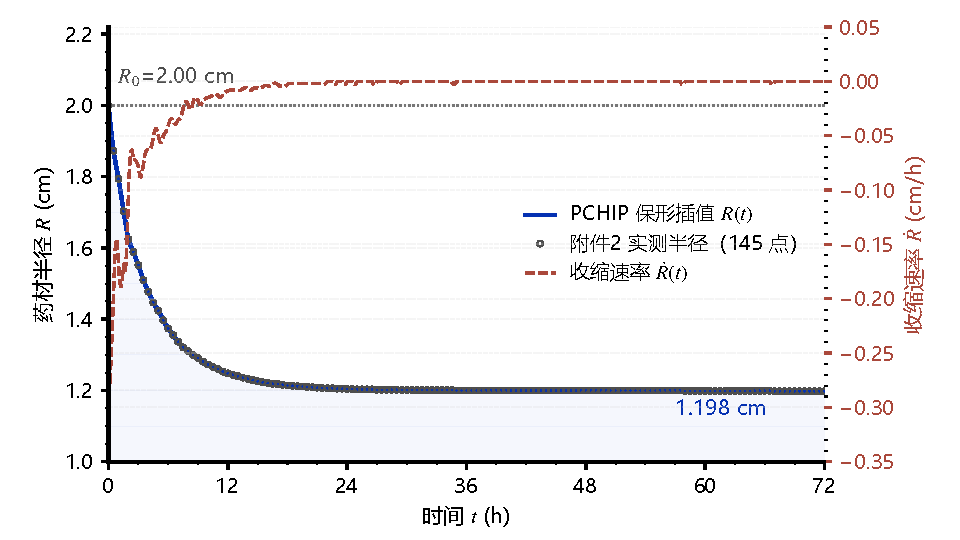
\includegraphics[width=0.9\textwidth,height=0.8\textheight,keepaspectratio]{figures/fig_input_shrinkage.pdf}
  \caption{附件 2 收缩半径的实测散点、单调化插值与收缩速率。半径由 $2.000$~cm 降至
  $1.198$~cm；PCHIP 分段三次插值配合累积取最小值的单调化处理，使 $R(t)$ 严格非增
  （单调化前后最大偏差 $2.2\times10^{-16}$~cm，即实测本身已单调）。右轴的 $\dot R(t)$
  是 Landau 变换对流项 $(1-\chi)\xi\dot R/R\,\partial_\xi\varphi$ 的直接输入。}
  \label{fig:input_shrinkage}
\end{figure}

\begin{figure}[H]
  \centering
  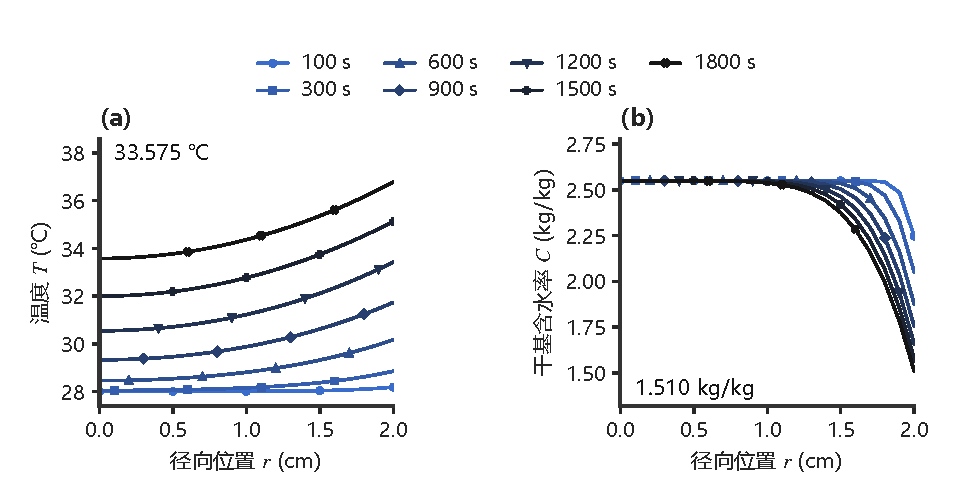
\includegraphics[width=0.9\textwidth,height=0.8\textheight,keepaspectratio]{figures/fig_q1_profiles.pdf}
  \caption{问题 1 前 $1800$~s 内温度与干基含水率的径向剖面。(a) 温度剖面自 $28~^\circ$C
  初值逐步抬升并保持表面高于中心的单调序；(b) 同期含水率剖面仅在表面薄层出现可见下降，
  中心处 $C$ 相对初值 $2.55$~kg/kg 仅降低 $1.0\times10^{-5}$~kg/kg。两图共用一条时刻色带，
  印证附录 2 常物性下"热先行、湿滞后"的时标分离。}
  \label{fig:q1_profiles}
\end{figure}

\begin{figure}[H]
  \centering
  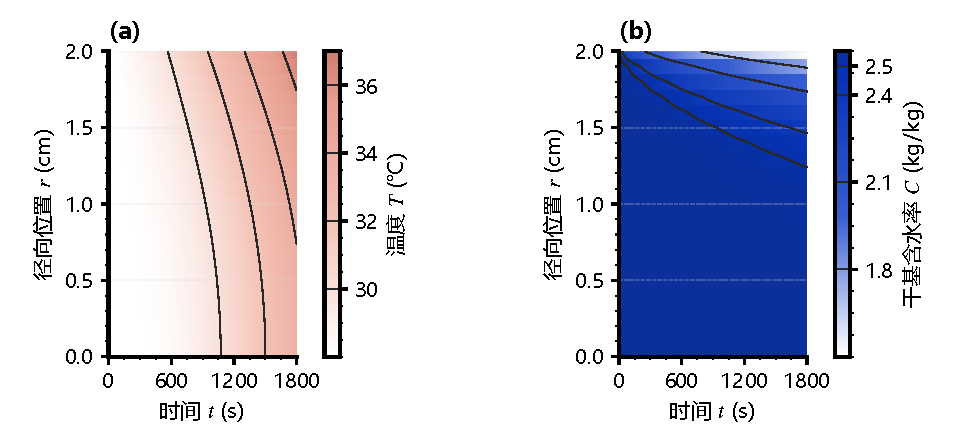
\includegraphics[width=0.9\textwidth,height=0.8\textheight,keepaspectratio]{figures/fig_q1_spacetime.pdf}
  \caption{问题 1 温度场与含水率场的时空（Hovm\"oller）分布。横轴为时间、纵轴为径向位置，
  叠加等值线便于读取梯度走向，各等值线的层级读数标在色标刻度上（图面不压字，避免遮挡场值）。
  温度场在 $1800$~s 内已铺满全径向，含水率场的可见变化仍局限在
  $r\gtrsim1.5$~cm 的外层（$r=1.5$~cm 处降幅 $0.174$~kg/kg，$r=0.7$~cm 处已不足
  $1.5\times10^{-3}$~kg/kg），二者的渗透深度差异是热扩散率与水分扩散系数量级悬殊的直接后果。}
  \label{fig:q1_spacetime}
\end{figure}

\begin{figure}[H]
  \centering
  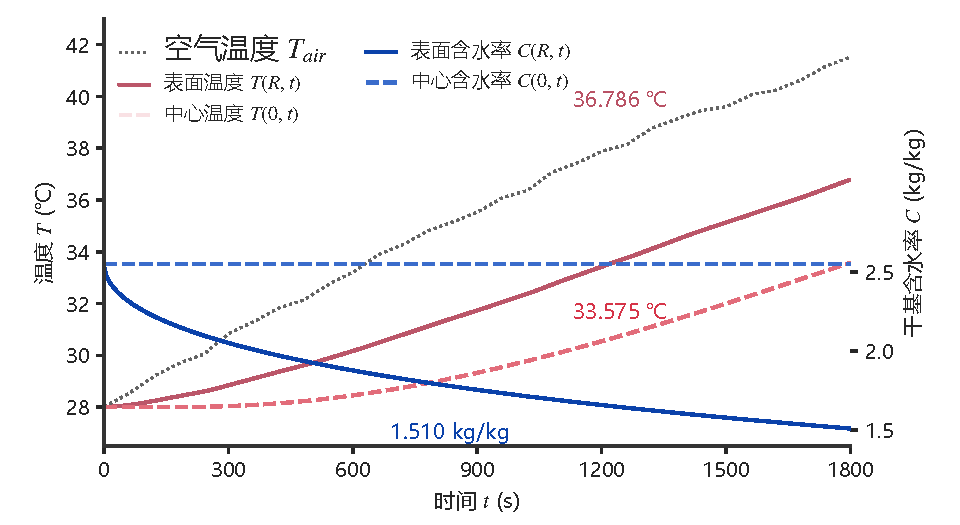
\includegraphics[width=0.9\textwidth,height=0.8\textheight,keepaspectratio]{figures/fig_q1_center_surface.pdf}
  \caption{问题 1 中心与表面测点的温度、含水率时程对照（双轴）。左轴三条温度曲线给出
  空气、表面、中心的层级顺序，右轴两条含水率曲线显示中心含水率在全程近乎水平。
  $t=1800$~s 时中心温度 $33.577~^\circ$C、表面温度 $36.786~^\circ$C，中心含水率
  $2.54999$~kg/kg。}
  \label{fig:q1_center_surface}
\end{figure}

\begin{figure}[H]
  \centering
  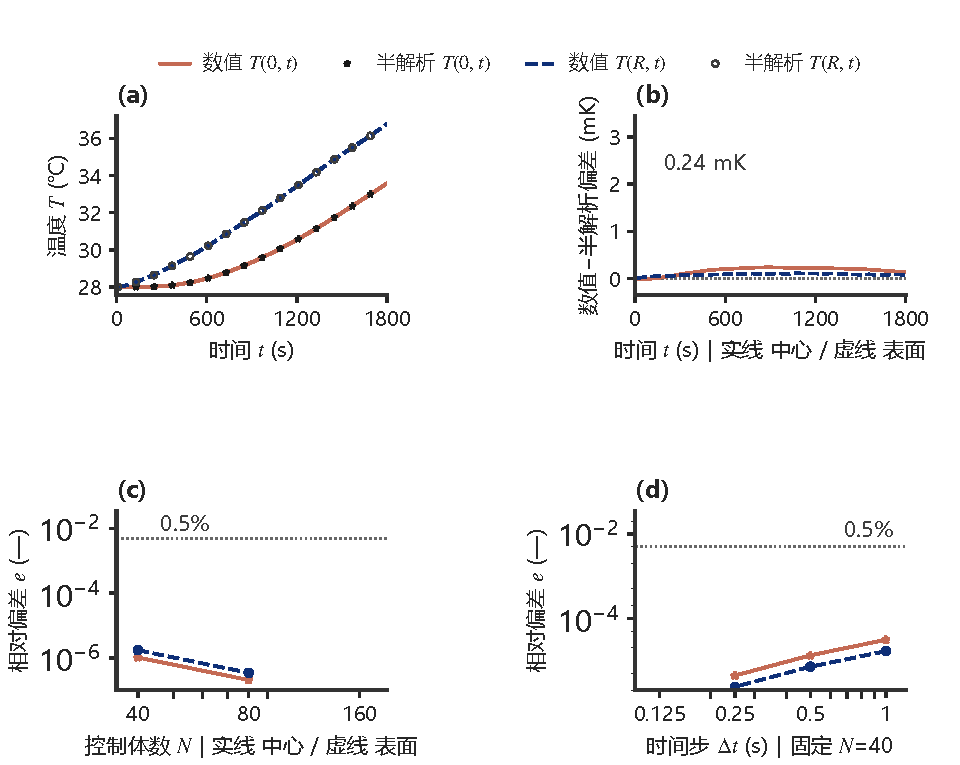
\includegraphics[width=0.9\textwidth,height=0.8\textheight,keepaspectratio]{figures/fig_q1_validation.pdf}
  \caption{问题 1 数值解的四项验证证据。(a) 数值解与 30 项 Bessel--Duhamel 半解析级数解
  逐点重合；(b) 两者偏差全程不超过 $1.97$~mK，量级与时间离散截断误差一致；
  (c) 网格加密收敛，交付网格 $N=40$ 相对 $N=160$ 参照解的偏差 $e_T=2.76\times10^{-5}$、
  $e_C=3.04\times10^{-4}$；(d) 时间步加密收敛，$\Delta t=1$~s 时 $e_T=2.45\times10^{-5}$。
  (c)(d) 中点线为 $0.5\%$ 判据线，四项均通过。}
  \label{fig:q1_validation}
\end{figure}

\begin{figure}[H]
  \centering
  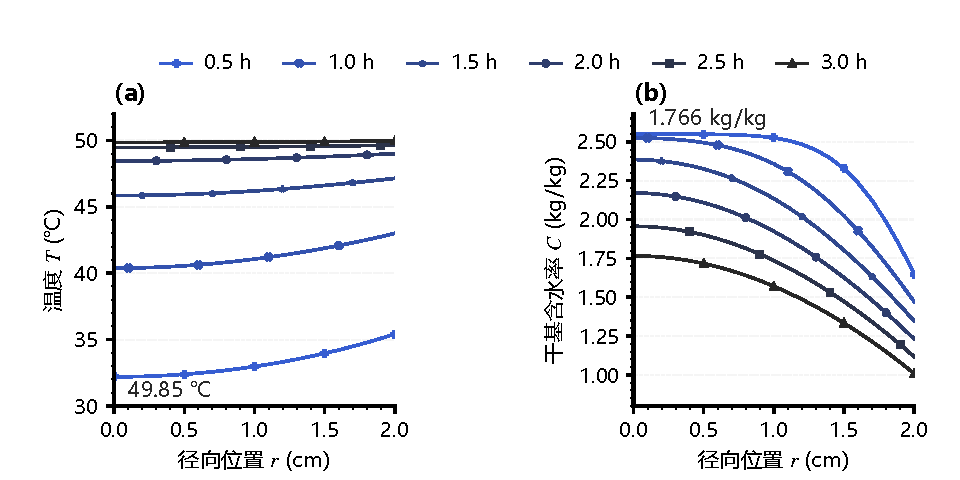
\includegraphics[width=0.9\textwidth,height=0.8\textheight,keepaspectratio]{figures/fig_q2_profiles.pdf}
  \caption{问题 2 前 $3$~h 内温度与含水率的径向剖面。改用附录 3 的温度--含水率耦合物性后，
  含水率下降已推进到可观深度：$t=3$~h 时中心温度 $49.849~^\circ$C、中心含水率
  $1.766$~kg/kg，与问题 1 常物性情形形成量级差别。}
  \label{fig:q2_profiles}
\end{figure}

\begin{figure}[H]
  \centering
  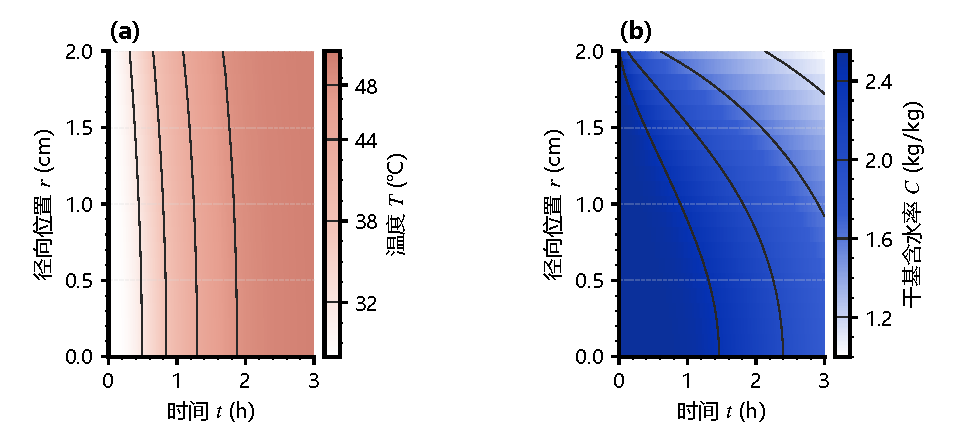
\includegraphics[width=0.9\textwidth,height=0.8\textheight,keepaspectratio]{figures/fig_q2_spacetime.pdf}
  \caption{问题 2 温度场与含水率场的时空分布，等值线层级读数同样标在色标刻度上。
  温度场在约 $1$~h 内基本追平空气平台温度，
  含水率场则呈现由表面向中心推进的干燥前沿。与图~\ref{fig:q1_spacetime} 同口径对比可见，
  耦合物性把水分响应的时标由"表层"量级拉到"全域"量级。}
  \label{fig:q2_spacetime}
\end{figure}

\begin{figure}[H]
  \centering
  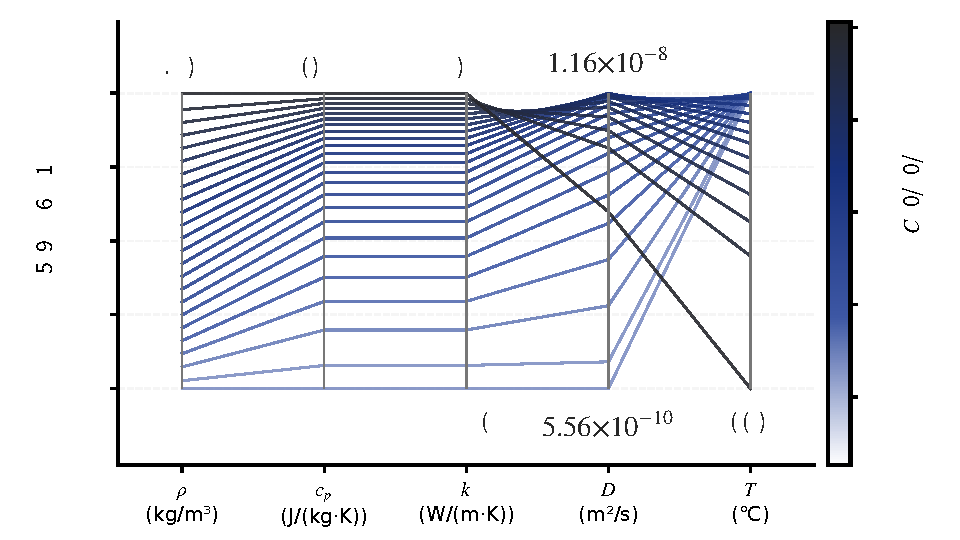
\includegraphics[width=0.9\textwidth,height=0.8\textheight,keepaspectratio]{figures/fig_q2_properties.pdf}
  \caption{附录 3 四项物性随含水率的联动（平行坐标）。样本取问题 3 全程节点场按含水率
  分 $24$ 箱的箱内均值，每条折线代表一个含水率区间的 $(\rho,c_p,k,D,T)$ 组合并按含水率
  着色；各轴按自身极值归一化，实际量程的上下端点分别标在该轴两端。随含水率由 $2.53$ 降到 $0.13$~kg/kg，
  $\rho$ 由 $973.7$ 降到 $666.8$~kg/m$^3$、$c_p$ 由 $3411$ 降到 $1765$~J/(kg$\cdot$K)、
  $k$ 由 $0.482$ 降到 $0.254$~W/(m$\cdot$K)，四项物性同向下降；$D$ 的最低值
  $5.70\times10^{-10}$~m$^2$/s 出现在最低含水率箱，即干燥后期扩散阻力上升，
  这是达标时间被拉长的主因。}
  \label{fig:q2_properties}
\end{figure}

\begin{figure}[H]
  \centering
  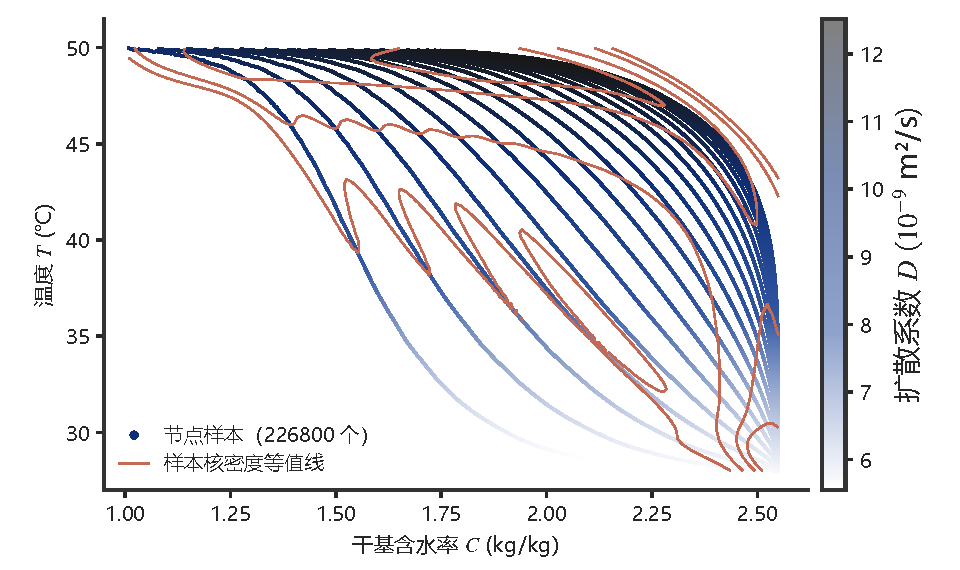
\includegraphics[width=0.9\textwidth,height=0.8\textheight,keepaspectratio]{figures/fig_q2_coupling_scatter.pdf}
  \caption{问题 2 全时空节点在 $(C,T)$ 平面上的分布，颜色编码局部水分扩散系数 $D$，
  叠加核密度等高线标出节点聚集区。$14801$ 个节点样本显示求解轨迹集中在两条带上：
  升温初期的高含水率带与准平台温度下的降湿带，二者交界即 $D$ 变化最剧烈的区域。}
  \label{fig:q2_coupling_scatter}
\end{figure}

\begin{figure}[H]
  \centering
  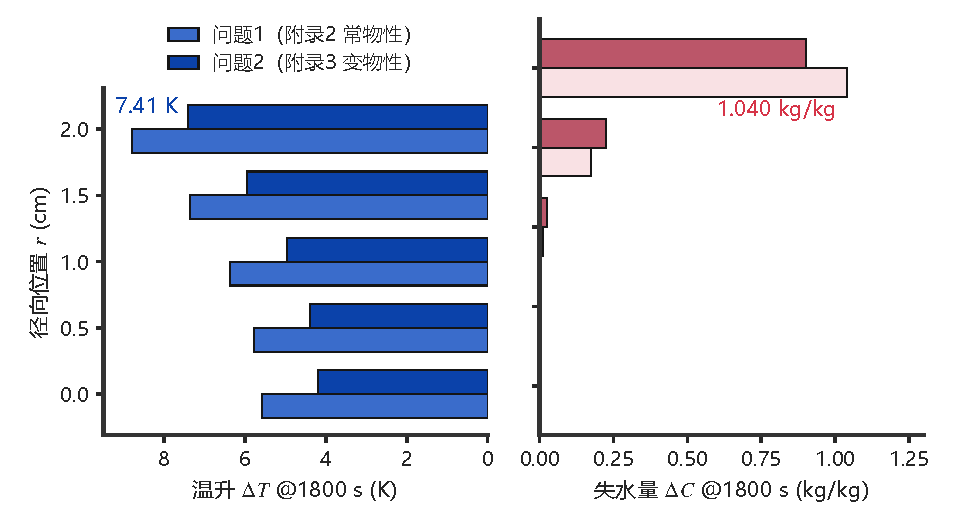
\includegraphics[width=0.9\textwidth,height=0.8\textheight,keepaspectratio]{figures/fig_q12_contrast.pdf}
  \caption{问题 1 与问题 2 在 $t=1800$~s 时的背靠背增量对比。左半为温升 $\Delta T$，
  右半为含水率降幅 $\Delta C$，按五个径向位置分列。温升差异始终在数摄氏度量级，
  而含水率降幅在中心处相差近一个量级（$1.0\times10^{-5}$ 对 $7.9\times10^{-5}$~kg/kg），
  在表面处则符号反转（$1.039$ 对 $0.901$~kg/kg，问题 1 反而更大）。这一"内部放大、表面反转"
  的格局说明物性口径切换主要改写水分方程的内部输运能力，而非能量方程。}
  \label{fig:q12_contrast}
\end{figure}

\begin{figure}[H]
  \centering
  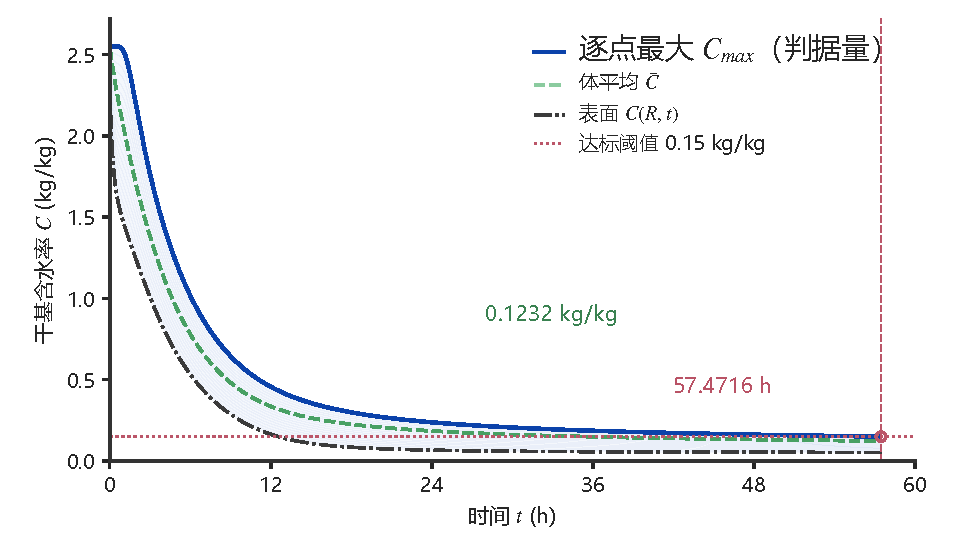
\includegraphics[width=0.9\textwidth,height=0.8\textheight,keepaspectratio]{figures/fig_q3_drying_curve.pdf}
  \caption{问题 3 干燥曲线与达标定位。逐点最大含水率 $C_{max}$ 是达标判据量，
  渐变带表示同一时刻药材内部由表面到最深处的含水率分布区间。
  $C_{max}$ 于 $t_{end}=56.709$~h 降至阈值 $0.15$~kg/kg，此时体平均含水率
  $0.1232$~kg/kg，说明按最保守的逐点判据定义的达标时间显著晚于按平均量判据的时间。}
  \label{fig:q3_drying_curve}
\end{figure}

\begin{figure}[H]
  \centering
  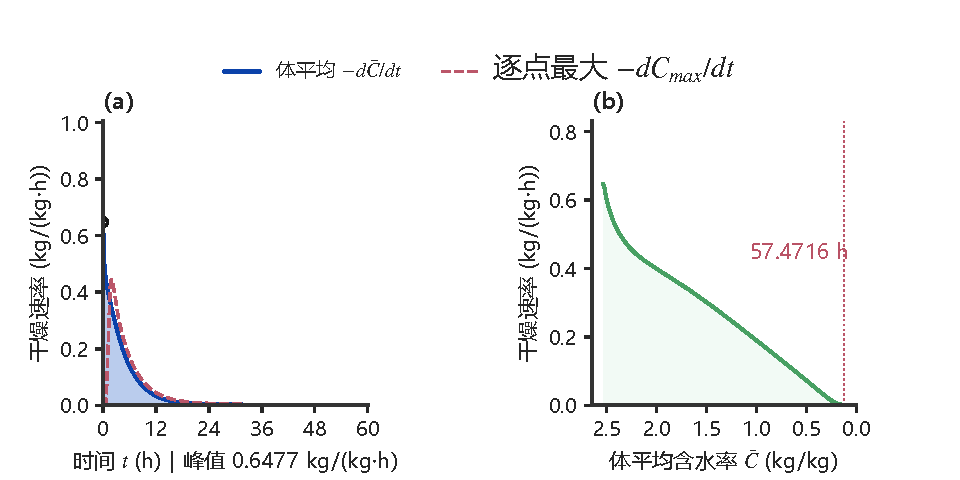
\includegraphics[width=0.9\textwidth,height=0.8\textheight,keepaspectratio]{figures/fig_q3_rate_curve.pdf}
  \caption{问题 3 干燥速率的两种读法。(a) 速率对时间：峰值 $0.6899$~kg/(kg$\cdot$h)
  出现在 $t=0$，此后单调衰减，说明本题不存在传统意义上的表面蒸发控制升速段；
  (b) 速率对体平均含水率（Krischer 口径，横轴反向以顺应干燥进程）。
  (b) 中不存在水平的恒速段，速率自始至终受内部扩散控制，这与附录 3 的 $D$ 强依赖
  含水率的形式一致。}
  \label{fig:q3_rate_curve}
\end{figure}

\begin{figure}[H]
  \centering
  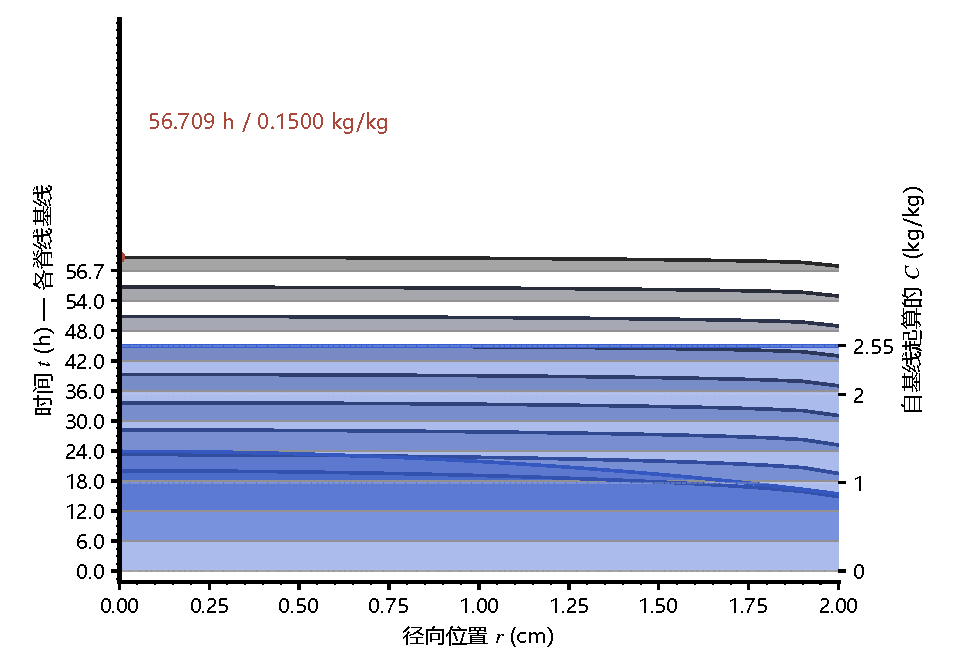
\includegraphics[width=0.9\textwidth,height=0.8\textheight,keepaspectratio]{figures/fig_q3_ridgeline.pdf}
  \caption{问题 3 含水率剖面的山脊图。每条脊线为一个时刻（每 $6$~h 取样，末条为
  $t_{end}$）的径向含水率分布，基线逐条下移以避免相互遮挡，右轴给出各脊线的公共幅值标尺。
  剖面形态由初期的近平坦逐步转为中心高、表面低的抛物型，末条脊线的峰值
  $0.1500$~kg/kg 即达标判据的临界状态。}
  \label{fig:q3_ridgeline}
\end{figure}

\begin{figure}[H]
  \centering
  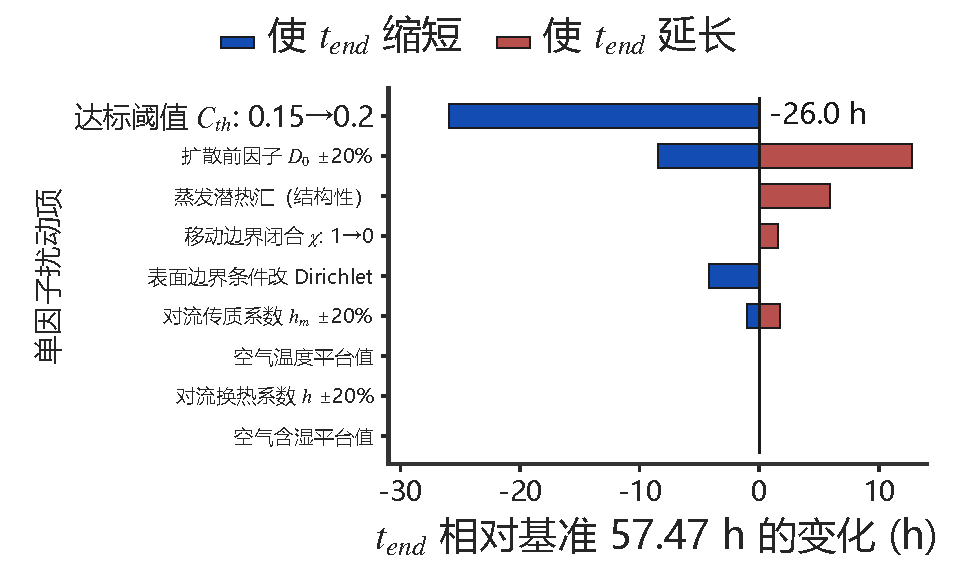
\includegraphics[width=0.9\textwidth,height=0.8\textheight,keepaspectratio]{figures/fig_q3_sensitivity.pdf}
  \caption{问题 3 达标时间的单因子（OFAT）灵敏度龙卷风图，基准 $t_{end}=56.18$~h
  （$N=20$ 灵敏度专用网格）。扩散前因子 $D_0$ 的 $\pm20\%$ 扰动带来 $-8.13$ 至
  $+12.31$~h 的变化，是最强的参数化不确定度来源；对流换热系数 $h$ 的同幅扰动仅带来
  $0.02$~h 量级变化。达标阈值 $C_{th}$ 由 $0.15$ 改到 $0.2$~kg/kg 会使 $t_{end}$
  缩短 $25.04$~h，属工艺定义变更而非模型误差。}
  \label{fig:q3_sensitivity}
\end{figure}

\begin{figure}[H]
  \centering
  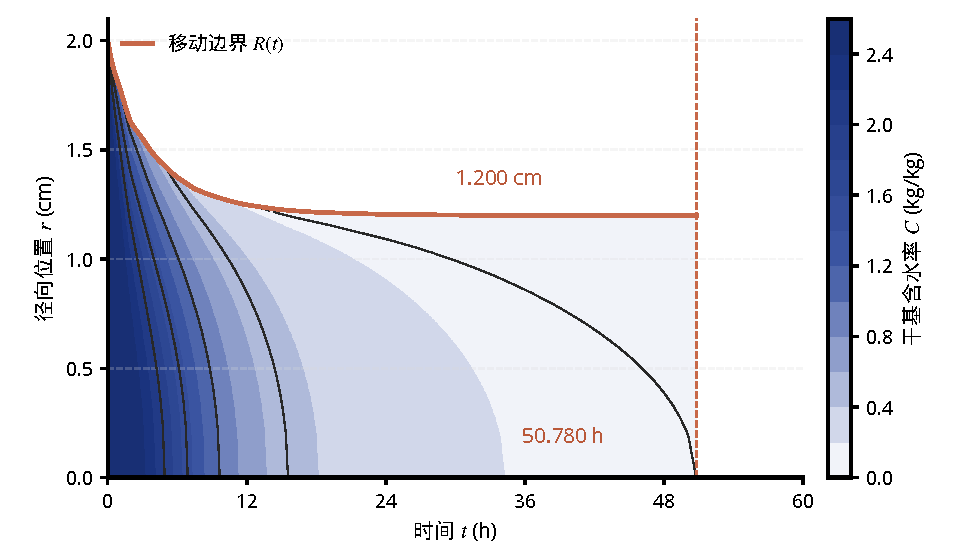
\includegraphics[width=0.9\textwidth,height=0.8\textheight,keepaspectratio]{figures/fig_q4_moving_boundary.pdf}
  \caption{问题 4 收缩域内含水率的时空分布与移动边界。等高线绘于物理坐标 $r$--$t$ 平面，
  边界外侧不作外推而留空，故图中色块的上缘即真实计算域。红线为 $R(t)$，由 $2.000$~cm
  收缩至 $1.200$~cm；竖虚线标出 $t_{end}=52.190$~h。域收缩与内部扩散同时进行，
  二者对达标时间的作用方向相反。}
  \label{fig:q4_moving_boundary}
\end{figure}

\begin{figure}[H]
  \centering
  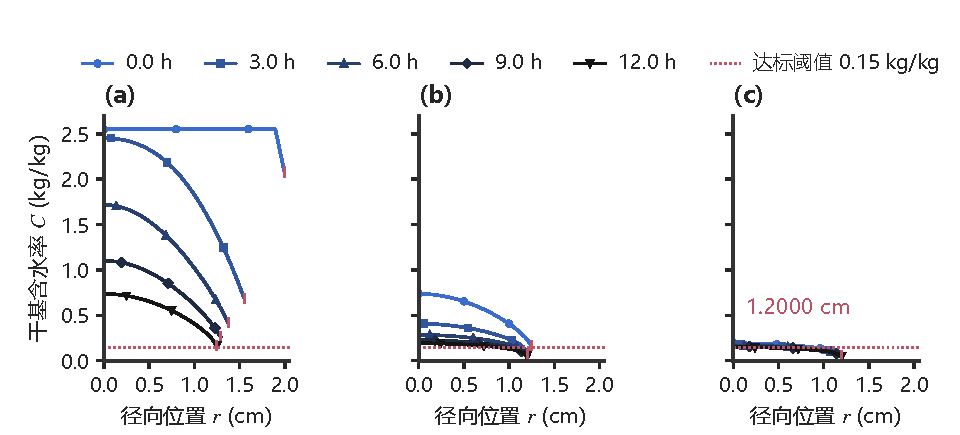
\includegraphics[width=0.9\textwidth,height=0.8\textheight,keepaspectratio]{figures/fig_q4_triptych.pdf}
  \caption{问题 4 含水率剖面按三个阶段分列，横轴为物理半径，故每条剖面的右端点即该时刻的
  $R(t)$。(a) $0$--$12$~h 边界收缩最快而剖面仍陡；(b) $12$--$36$~h 剖面整体下移；
  (c) $36$~h 至 $t_{end}$ 剖面趋于平坦并触及阈值线，末态半径 $1.200$~cm。
  竖短线标出各时刻表面位置，可见收缩域与剖面演化的同步关系。}
  \label{fig:q4_triptych}
\end{figure}

\begin{figure}[H]
  \centering
  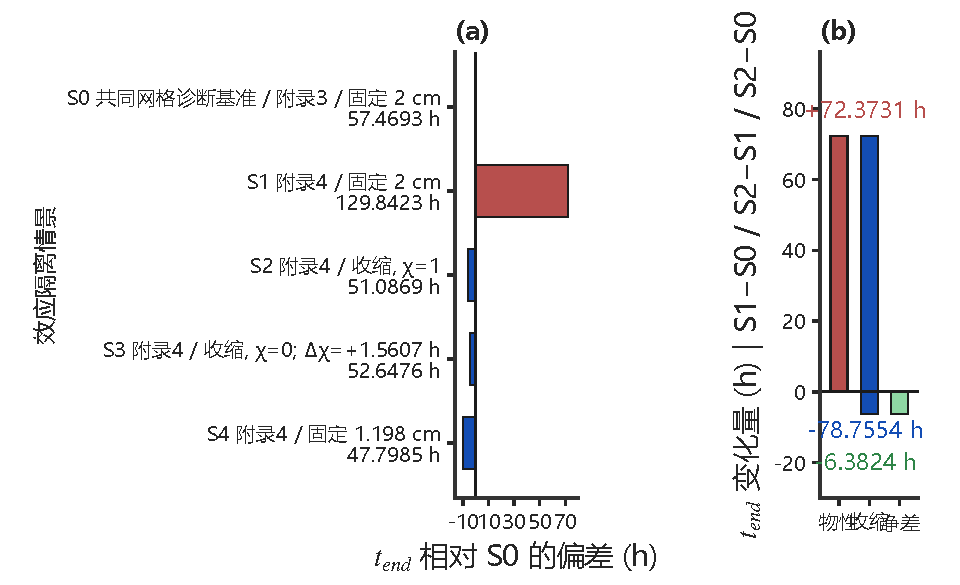
\includegraphics[width=0.9\textwidth,height=0.8\textheight,keepaspectratio]{figures/fig_q4_shrink_effect.pdf}
  \caption{问题 4 的效应隔离与加性分解。(a) 五个情景相对问题 3 基线 S0 的 $t_{end}$ 偏差：
  仅把物性换成附录 4（S1）使达标时间延长到 $128.594$~h，再引入收缩（S2）回落到
  $52.190$~h。(b) 按式 (24) 的加性分解：换物性 $+71.885$~h、加收缩 $-76.404$~h、
  净差 $-4.519$~h，加性恒等式残差 $7.11\times10^{-15}$~h。两项效应量级相当而符号相反，
  故净效应远小于单项效应。}
  \label{fig:q4_shrink_effect}
\end{figure}

\begin{figure}[H]
  \centering
  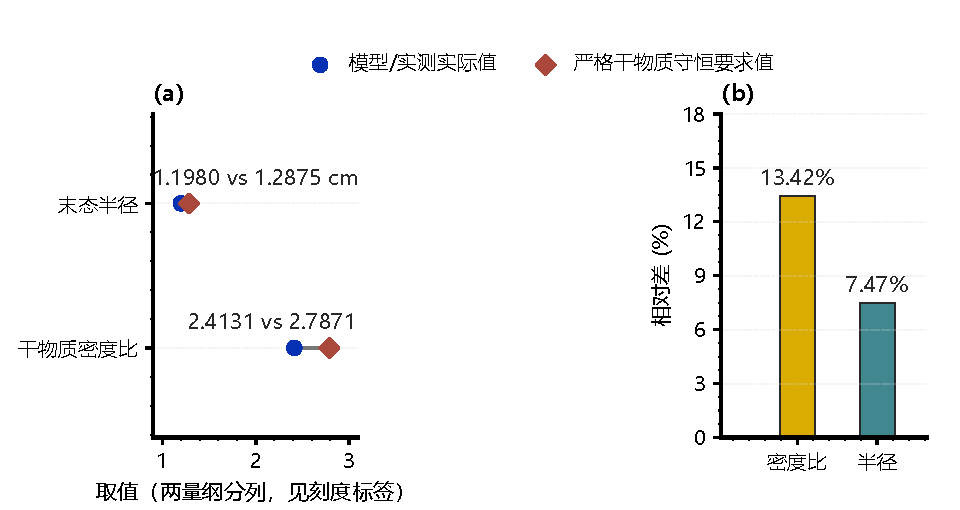
\includegraphics[width=0.9\textwidth,height=0.8\textheight,keepaspectratio]{figures/fig_q4_mass_consistency.pdf}
  \caption{附录 4 密度关系与附件 2 收缩数据的干物质自洽性诊断（INC1）。(a) 两个口径的
  配对比较：图中刻度「干物质密度比」的完整口径为干物质表观密度比
  $\rho_s(C_{th})/\rho_s(C_0)$，实际值 $2.4131$ 对严格守恒要求值 $2.7871$；
  实测末态半径 $1.1980$~cm 对由密度守恒反演的 $1.2875$~cm。(b) 两口径的相对差分别为
  $13.42\%$ 与 $7.47\%$。该不相容度只作为题面数据的诊断量报告，不参与求解，
  交付解仍以附件 2 实测 $R(t)$ 为准。}
  \label{fig:q4_mass_consistency}
\end{figure}

\begin{figure}[H]
  \centering
  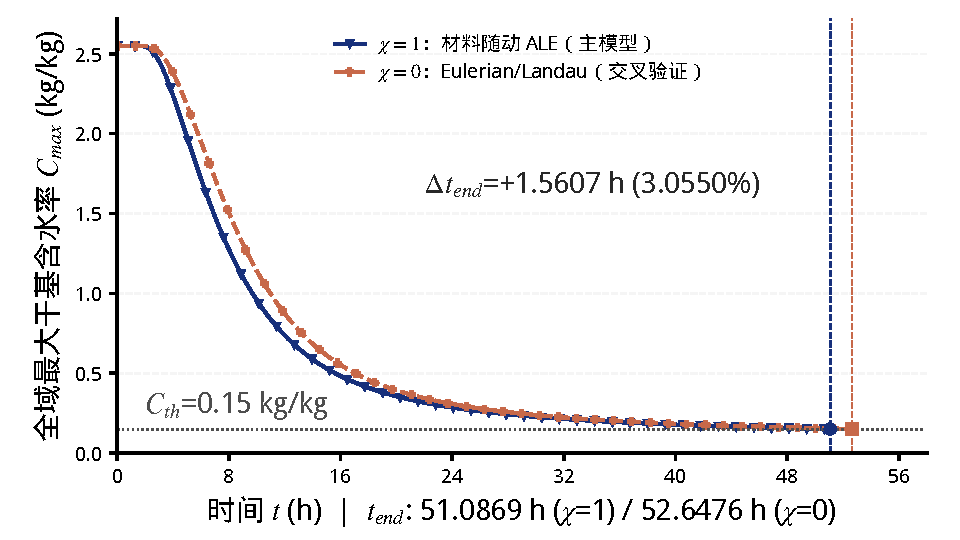
\includegraphics[width=0.9\textwidth,height=0.8\textheight,keepaspectratio]{figures/fig_chi_closure.pdf}
  \caption{问题 4 移动边界闭合方式的不确定度。$\chi=0$（网格随边界同步收缩，交付口径）
  给出 $t_{end}=52.190$~h，$\chi=1$（边界收缩不携带对流输运）给出 $50.694$~h，
  相差 $-1.496$~h 即 $-2.87\%$。两条 $C_{max}(t)$ 曲线在全程几乎重合，
  说明闭合方式的选择在本题参数下属次要不确定度。}
  \label{fig:chi_closure}
\end{figure}

\begin{figure}[H]
  \centering
  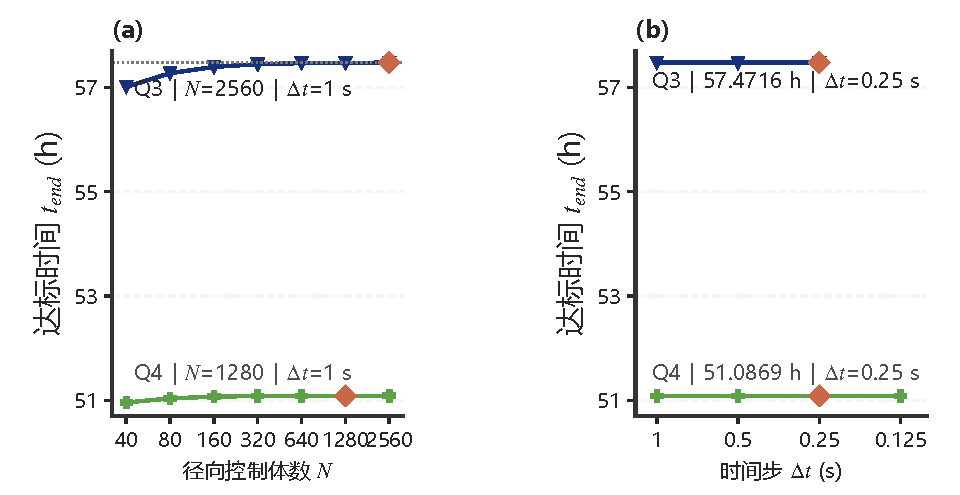
\includegraphics[width=0.9\textwidth,height=0.8\textheight,keepaspectratio]{figures/fig_convergence.pdf}
  \caption{交付网格的收敛性证据，口径为附录 3 物性、固定半径。(a) 达标时间随控制体数
  $N$ 的变化：$N=40$ 相对 $N=80$ 的相对变化 $0.458\%$，落在 $1\%$ 判据内，
  故取 $N=40$ 为交付网格（图中菱形）。
  (b) 相对质量收支残差随 $N$ 均在 $10^{-14}$ 量级，比 $10^{-10}$ 容差低约四个量级，
  说明离散格式严格守恒，网格误差来自截断而非守恒破坏。}
  \label{fig:convergence}
\end{figure}

\begin{figure}[H]
  \centering
  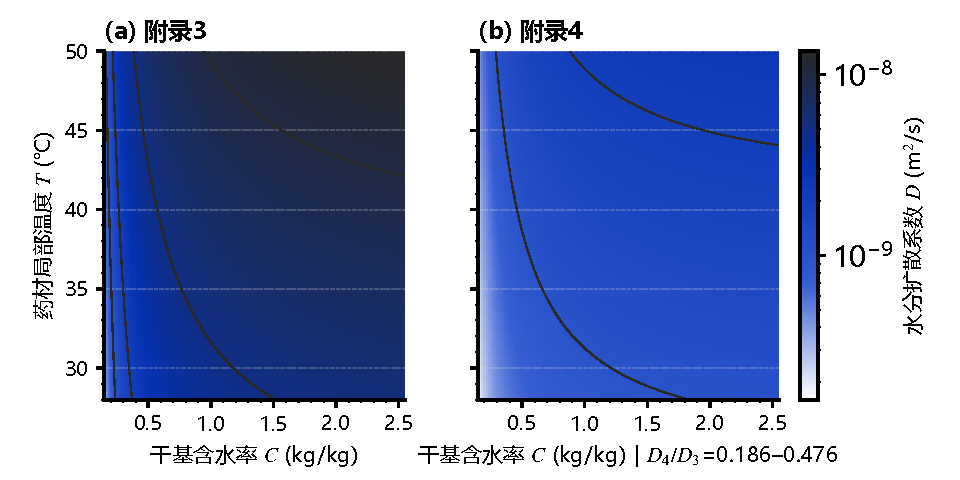
\includegraphics[width=0.9\textwidth,height=0.8\textheight,keepaspectratio]{figures/fig_property_maps.pdf}
  \caption{附录 3 与附录 4 的水分扩散系数 $D(C,T)$ 在 $[0.15,2.55]\times[28,50]$
  上的分布（共享对数色标，叠加等值线）。(a) 附录 3 的 $D$ 覆盖
  $3.35\times10^{-10}$--$1.35\times10^{-8}$~m$^2$/s；(b) 附录 4 覆盖
  $1.59\times10^{-10}$--$2.50\times10^{-9}$~m$^2$/s。比值 $D_4/D_3$ 在
  $0.186$--$0.476$ 之间，即附录 4 的扩散能力系统性低于附录 3，
  这正是图~\ref{fig:q4_shrink_effect} 中 S1 情景达标时间大幅延长的成因。}
  \label{fig:property_maps}
\end{figure}

% ============================================================================
% 以下 7 张为非数据类示意图（HTML+CSS 转矢量 PDF 3 张 + TikZ 4 张）。
% 图内一律不含数值结果与结论措辞，口径与结论全部写在 caption 里。
% 全部为纯黑白线稿：层次由线宽、虚实与留白承担，不依赖颜色，灰度打印等效可读。
% ============================================================================

\begin{figure}[H]
  \centering
  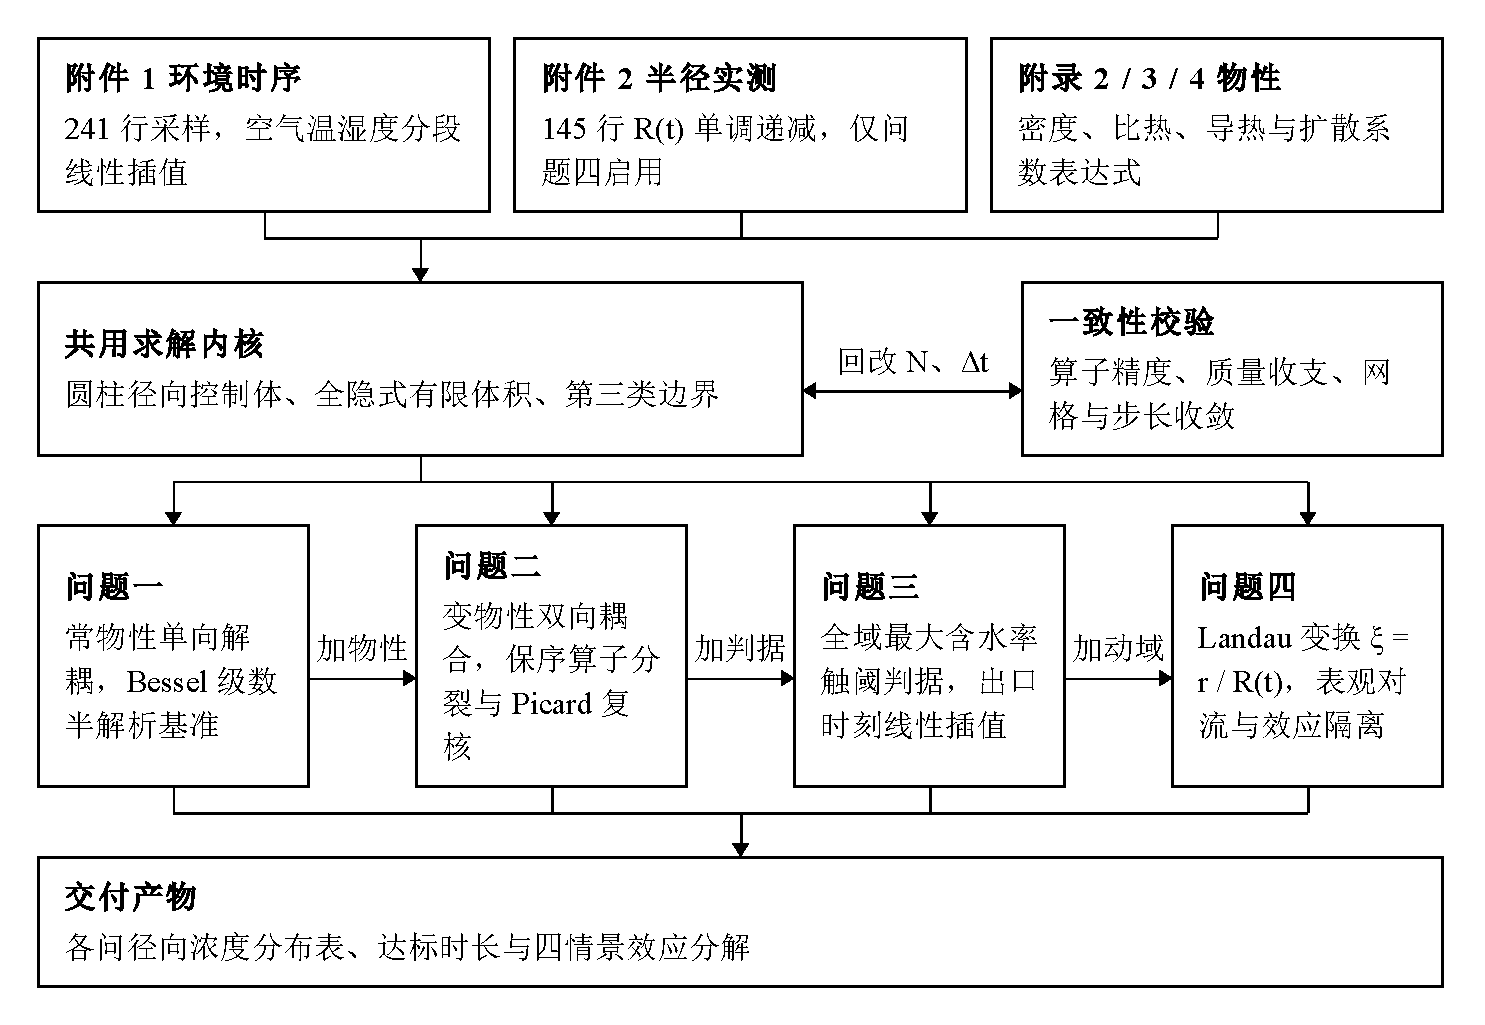
\includegraphics[width=0.98\textwidth,height=0.8\textheight,keepaspectratio]{figures/fig_roadmap.pdf}
  \caption{全文建模路线。三份题给材料（附件 1 环境时序、附件 2 半径实测、
  附录 2--4 物性表达式）汇入同一个求解内核：圆柱径向控制体 + 全隐式有限体积 +
  第三类边界。内核与一致性校验之间是双向边——算子精度、质量收支与网格/步长收敛
  一旦不达标即回改控制体数 $N$ 与时间步长 $\Delta t$，而非调参凑结果。
  四问不是并列任务而是\textbf{渐进承接链}：问题一在常物性下单向解耦并用 Bessel 级数
  提供半解析基准，问题二加变物性形成双向耦合，问题三加触阈判据，问题四加动域。
  每一步只新增一项机制，使后一问的差异可归因到该项机制上。}
  \label{fig:roadmap}
\end{figure}

\begin{figure}[H]
  \centering
  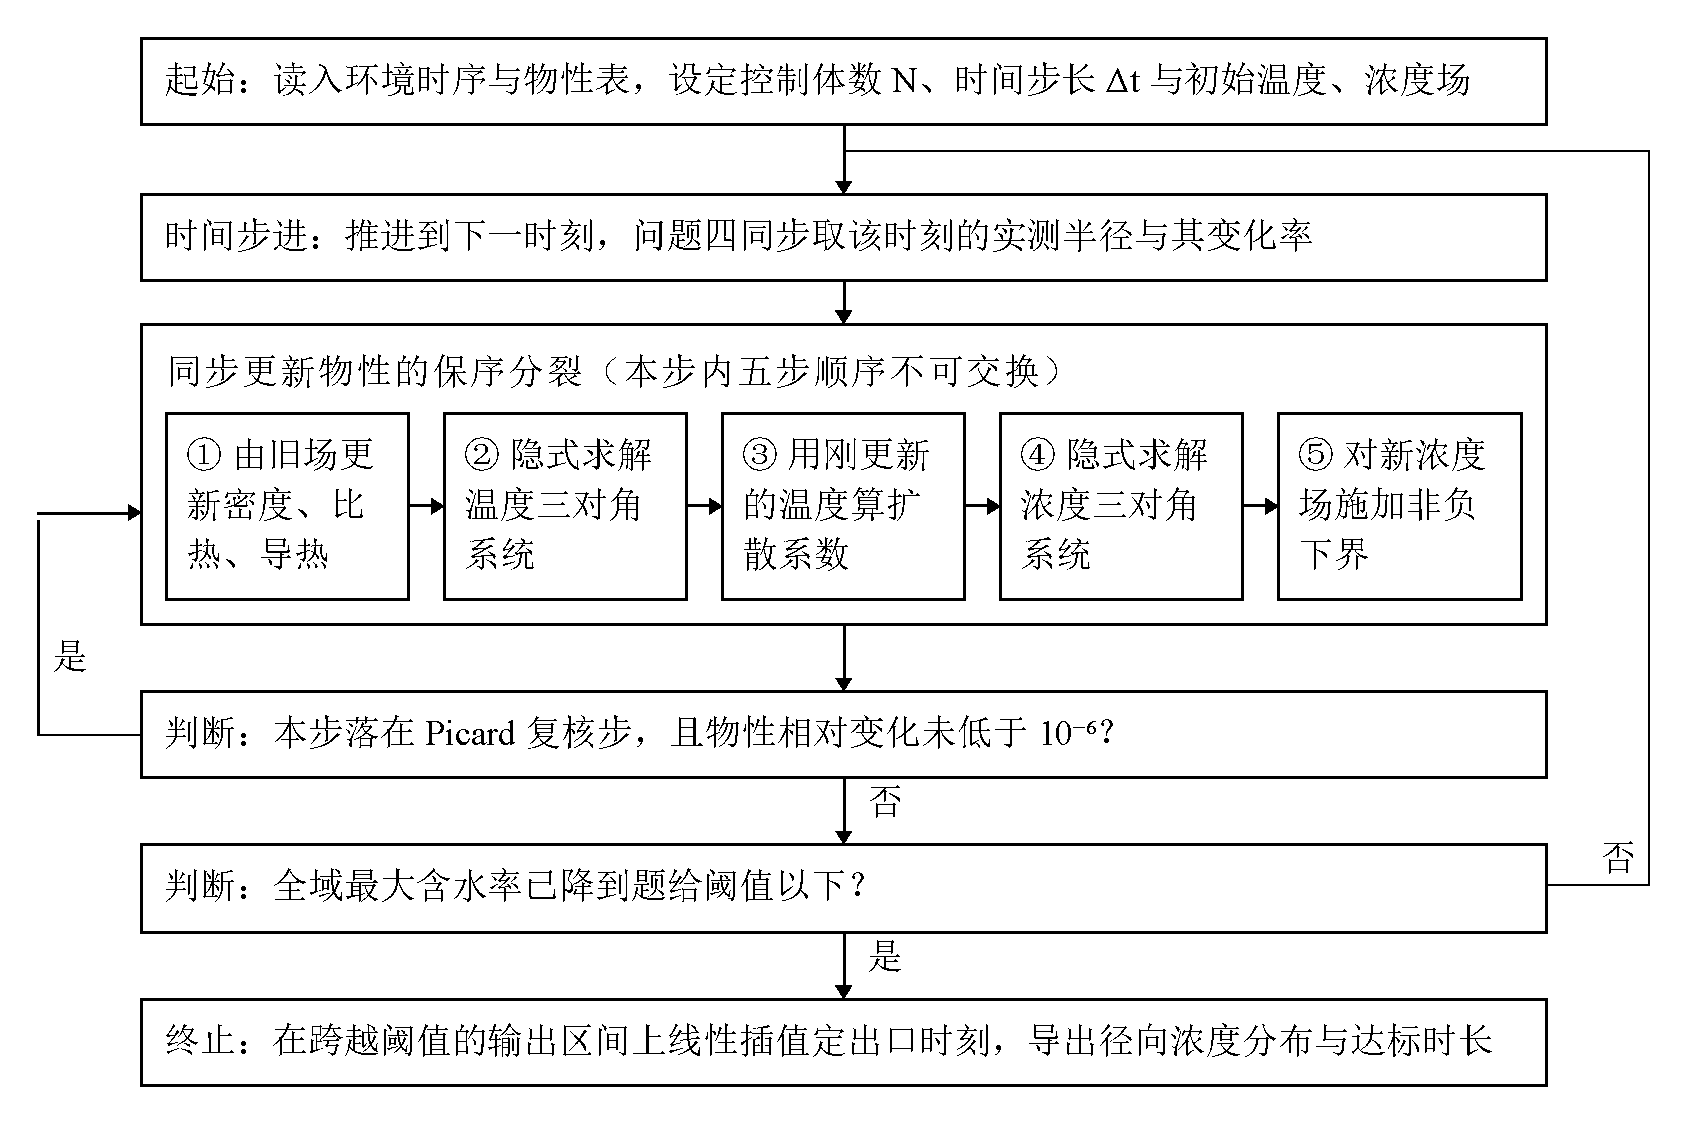
\includegraphics[width=0.96\textwidth,height=0.8\textheight,keepaspectratio]{figures/fig_pipeline.pdf}
  \caption{单个时间步内的求解流程。核心是\textbf{保序算子分裂}：五个子步的次序不可交换——
  ① 用旧场更新密度、比热、导热，② 隐式解温度三对角系统，③ 用\emph{刚更新的}温度算
  扩散系数，④ 隐式解浓度三对角系统，⑤ 对新浓度场施加非负下界。若把 ③ 提到 ② 之前，
  扩散系数就退化为用旧温度计算，耦合被人为削弱。图中两条回路分工不同：左侧回路是
  Picard 复核（每隔若干步复算物性，直至相对变化低于 $10^{-6}$），右侧回路是时间推进。
  终止判据只在 Picard 收敛后检查，避免用未收敛的中间场触发停机。}
  \label{fig:pipeline}
\end{figure}

\begin{figure}[H]
  \centering
  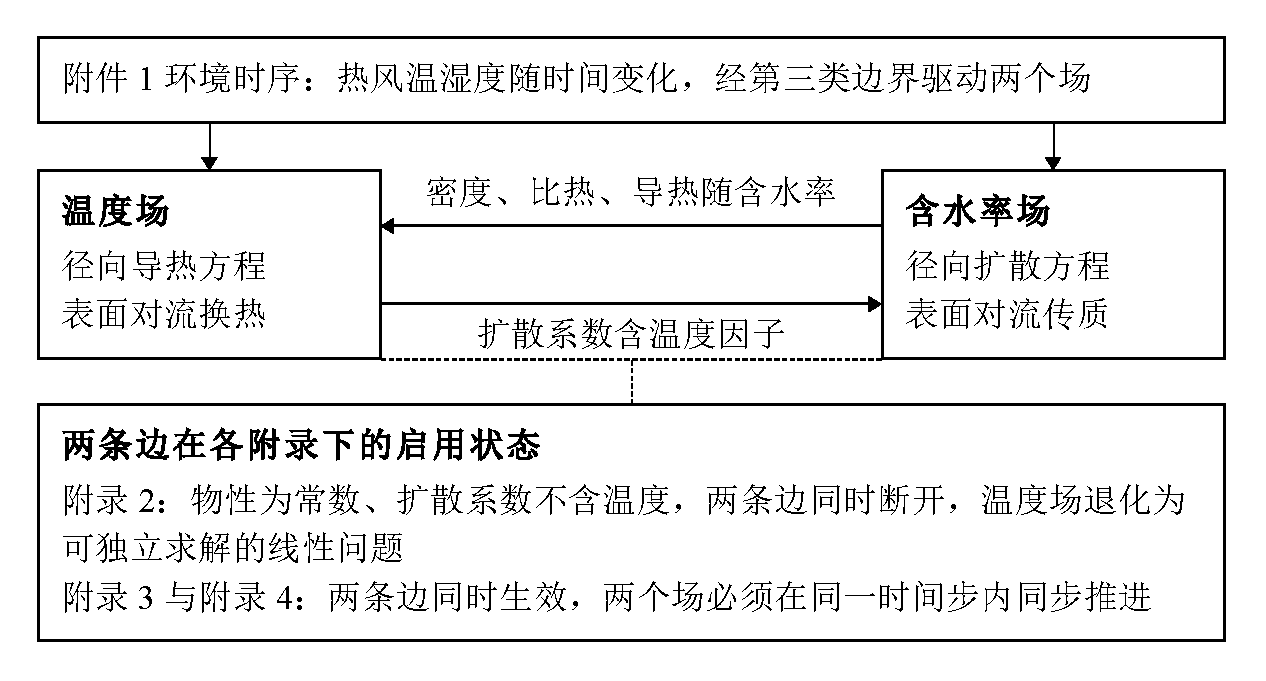
\includegraphics[width=0.9\textwidth,height=0.8\textheight,keepaspectratio]{figures/fig_coupling_structure.pdf}
  \caption{温度场与含水率场的耦合结构。附件 1 的热风温湿度经第三类边界同时驱动两个场，
  两场之间是一个\textbf{双向环}：向左的边是物性依赖（密度、比热、导热随含水率变化），
  向右的边是扩散系数中的温度因子。这两条边的启用状态决定了问题的数学类型——
  附录 2 下物性为常数且扩散系数不含温度，两条边同时断开，温度场退化为可独立求解的
  线性问题；附录 3 与附录 4 下两条边同时生效，两个场必须在同一时间步内同步推进，
  不能先算完整条温度时程再算浓度。虚线为注记引出线，不代表信息流。}
  \label{fig:coupling_structure}
\end{figure}

\begin{figure}[H]
  \centering
  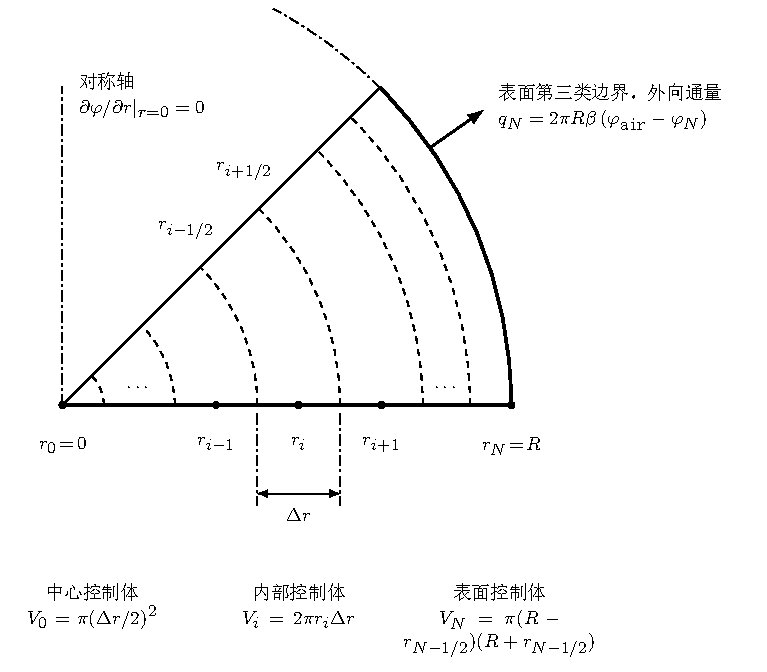
\includegraphics[width=0.8\textwidth,height=0.8\textheight,keepaspectratio]{figures/tikz_cylinder_cv.pdf}
  \caption{圆柱径向有限体积的控制体划分。扇形只画出横截面的一部分（点划弧示意其余
  部分同构），虚线弧为控制体界面 $r_{i\pm1/2}$，实心圆点为网格结点。三类控制体的体积
  写法互不相同：轴心处 $V_0=\pi(\Delta r/2)^2$ 是实心小圆盘，内部 $V_i=2\pi r_i\Delta r$
  含向心汇聚因子 $r_i$，表面 $V_N=\pi(R-r_{N-1/2})(R+r_{N-1/2})$ 是半宽环。注意：若照搬
  直角坐标的等体积划分，会系统性低估中心区域的升温与失水速率。表面控制体的外向通量由第三类边界
  $q_N=2\pi R\beta(\varphi_{\mathrm{air}}-\varphi_N)$ 给出，
  轴心处则由对称条件 $\partial\varphi/\partial r|_{r=0}=0$ 关闭。}
  \label{fig:cylinder_cv}
\end{figure}

\begin{figure}[H]
  \centering
  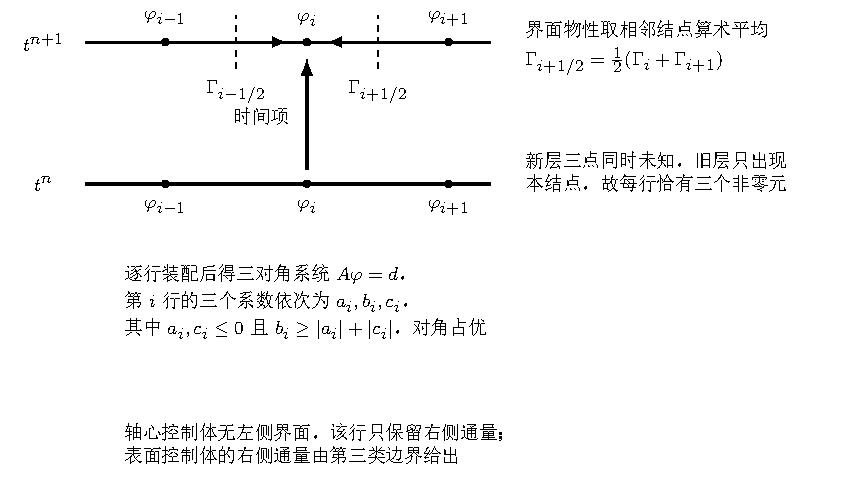
\includegraphics[width=0.9\textwidth,height=0.8\textheight,keepaspectratio]{figures/tikz_fv_stencil.pdf}
  \caption{全隐式有限体积的两时间层耦合模板。新层 $t^{n+1}$ 上三个结点同时未知
  （两条水平箭头表示两侧界面通量都指向待解结点），旧层 $t^{n}$ 只有\emph{同一结点}
  进入右端项，因此每行恰有三个非零元，逐行装配即得三对角系统，可用 Thomas 算法
  $O(N)$ 求解。界面物性取相邻结点算术平均 $\Gamma_{i+1/2}=\tfrac12(\Gamma_i+\Gamma_{i+1})$。
  系数满足 $a_i,c_i\le0$ 且 $b_i\ge|a_i|+|c_i|$，即对角占优——这是全隐式格式无条件稳定、
  且不会产生非物理振荡的代数根据。轴心行无左侧界面故只保留右侧通量，
  表面行的右侧通量由第三类边界替换。}
  \label{fig:fv_stencil}
\end{figure}

\begin{figure}[H]
  \centering
  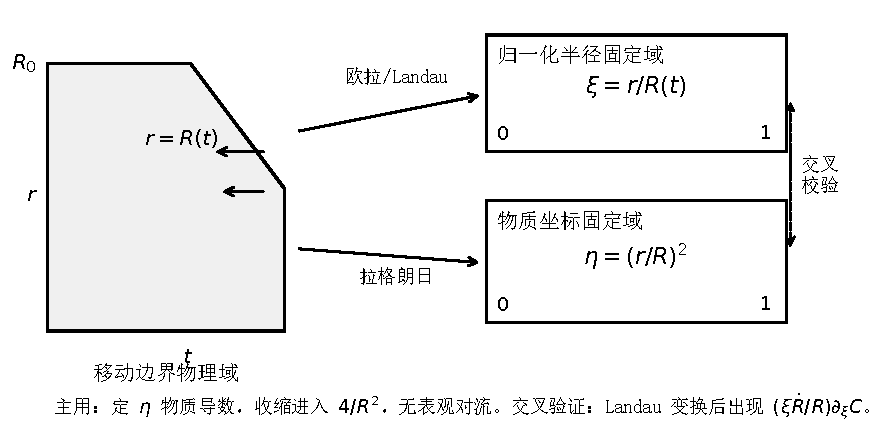
\includegraphics[width=0.8\textwidth,height=0.8\textheight,keepaspectratio]{figures/tikz_landau_map.pdf}
  \caption{Landau 变换 $\xi=r/R(t)$ 把收缩的物理域映成固定计算域。上两排为物理域在
  $t^{n}$ 与 $t^{n+1}$ 两个时刻的样子：域端点内移（$\dot R<0$），网格随之被压缩，
  结点的物理位置逐步变化；下排为计算域，端点恒为 $0$ 与 $1$，结点数与间距全程固定，
  因此可以套用与固定域完全相同的三对角装配。代价体现在方程上：定 $\xi$ 求导与定 $r$
  求导相差 $\xi\dot R(t)\,\partial\varphi/\partial r$，该差项进入计算域方程后表现为
  表观对流项 $(1-\chi)(\xi\dot R/R)\partial C/\partial\xi$。注意：该项须用一阶迎风离散：
  $\dot R<0$ 使对流指向 $\xi$ 减小方向，迎风侧为较大 $\xi$；表面附近网格 Péclet 数
  可超过 $2$，中心差分会产生振荡。}
  \label{fig:landau_map}
\end{figure}

\begin{figure}[H]
  \centering
  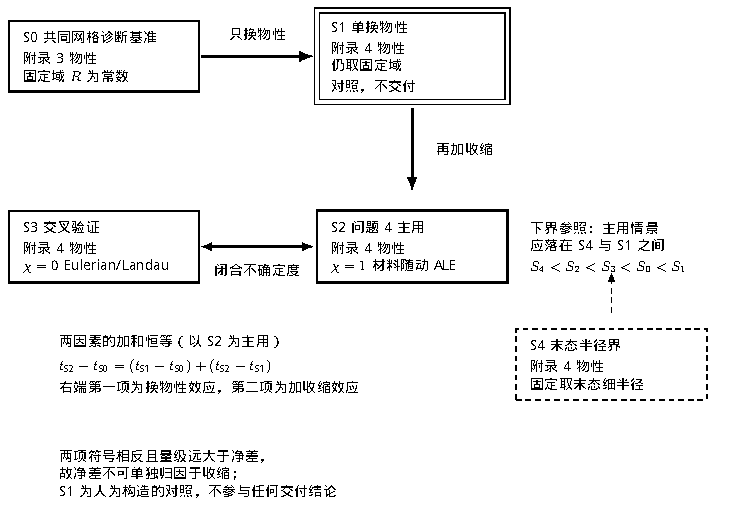
\includegraphics[width=0.9\textwidth,height=0.8\textheight,keepaspectratio]{figures/tikz_effect_isolation.pdf}
  \caption{问题 4 相对问题 3 的两因素效应隔离路径。问题 4 同时改变了两件事
  （附录 3$\to$附录 4 的物性、固定域$\to$收缩域），直接对比时长并归因于「收缩使干燥
  加快」是典型的混淆归因。故按「单因素改变、其他量固定」构造情景链：S0 基线
  $\to$ S1 只换物性 $\to$ S2 再加收缩，两步之差满足加和恒等
  $t_{\mathrm{S2}}-t_{\mathrm{S0}}=(t_{\mathrm{S1}}-t_{\mathrm{S0}})+(t_{\mathrm{S2}}-t_{\mathrm{S1}})$。
  S3 为骨架运动学的替代闭合（$\chi=1$ 仿射骨架），与主用的 $\chi=0$ 之差作为模型
  不确定度报告，不合并成单一数字。S4（虚线框）以末态细半径的固定域求解，给出时长
  下界参照。注意：S1 用双线框标出：它用附录 4 的慢扩散却不允许收缩，物理上不自洽，
  是\emph{人为构造的对照情景}，其时长豁免合理区间审计，且不得作为任何交付结论。
  两项效应符号相反、量级均远大于净差，五情景的具体时长见
  图~\ref{fig:q4_shrink_effect}。}
  \label{fig:effect_isolation}
\end{figure}

%       或按需把下面单个 figure 环境复制到对应章节。
% 说明：全部为矢量 PDF，插入宽度统一 0.90\textwidth（各图长宽比同属一档）。
%       图内只保留必要数值与短锚点，口径/结论一律写在下方 caption 里。

\begin{figure}[H]
  \centering
  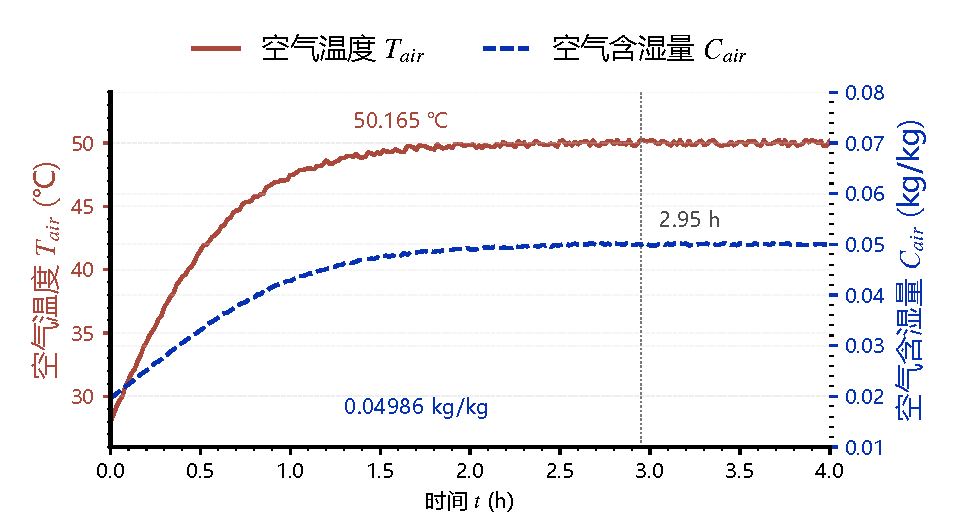
\includegraphics[width=0.9\textwidth,height=0.8\textheight,keepaspectratio]{figures/fig_input_chamber.pdf}
  \caption{附件 1 干燥室工况的双轴时程。左轴为空气温度 $T_{air}(t)$，右轴为空气含湿量
  $C_{air}(t)$。温度自 $28~^\circ$C 快速抬升，$1.37$~h 已达 $49~^\circ$C，
  峰值 $50.246~^\circ$C 出现在 $2.95$~h，随后进入平台段；含湿量峰值 $0.05025$~kg/kg。
  该平台值即问题 2--4 长时程求解所用的边界驱动。两轴量程刻意错开，使两族曲线各占一个
  纵向带，避免读图时混淆归属。}
  \label{fig:input_chamber}
\end{figure}

\begin{figure}[H]
  \centering
  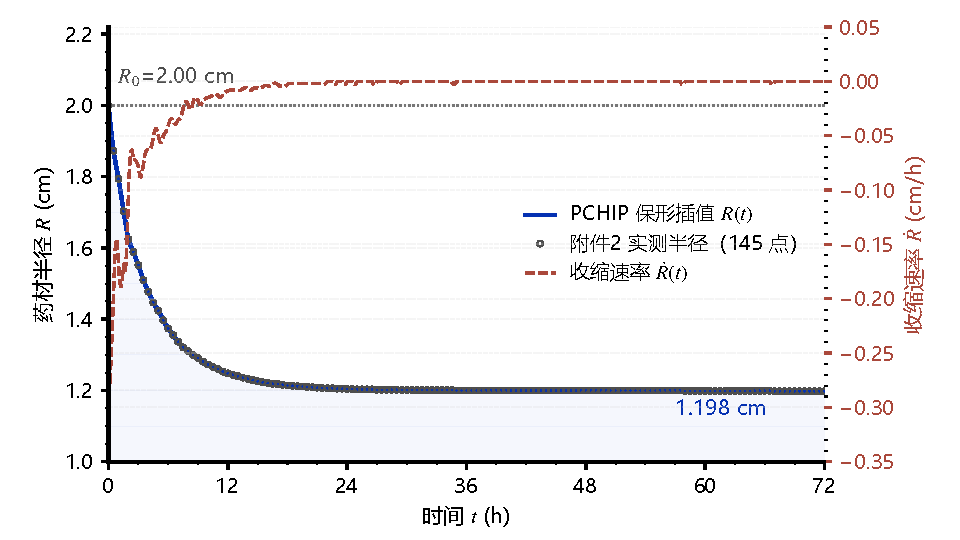
\includegraphics[width=0.9\textwidth,height=0.8\textheight,keepaspectratio]{figures/fig_input_shrinkage.pdf}
  \caption{附件 2 收缩半径的实测散点、单调化插值与收缩速率。半径由 $2.000$~cm 降至
  $1.198$~cm；PCHIP 分段三次插值配合累积取最小值的单调化处理，使 $R(t)$ 严格非增
  （单调化前后最大偏差 $2.2\times10^{-16}$~cm，即实测本身已单调）。右轴的 $\dot R(t)$
  是 Landau 变换对流项 $(1-\chi)\xi\dot R/R\,\partial_\xi\varphi$ 的直接输入。}
  \label{fig:input_shrinkage}
\end{figure}

\begin{figure}[H]
  \centering
  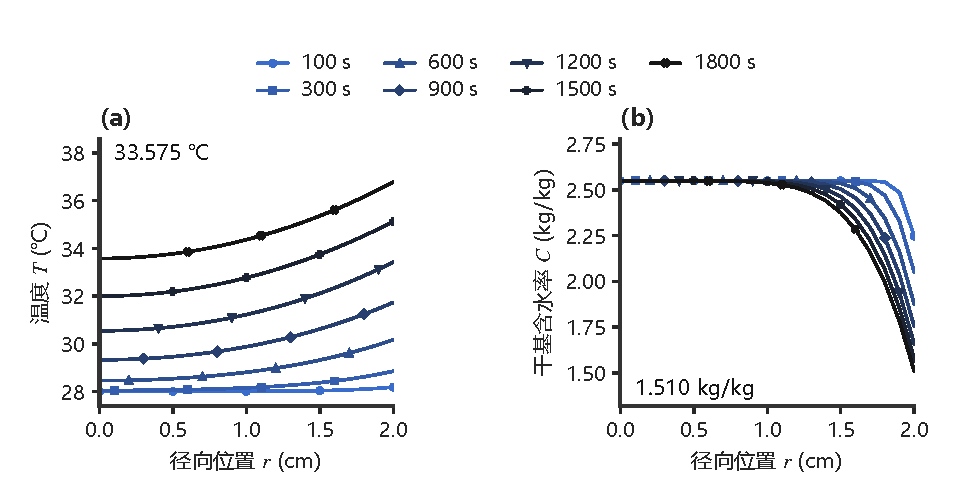
\includegraphics[width=0.9\textwidth,height=0.8\textheight,keepaspectratio]{figures/fig_q1_profiles.pdf}
  \caption{问题 1 前 $1800$~s 内温度与干基含水率的径向剖面。(a) 温度剖面自 $28~^\circ$C
  初值逐步抬升并保持表面高于中心的单调序；(b) 同期含水率剖面仅在表面薄层出现可见下降，
  中心处 $C$ 相对初值 $2.55$~kg/kg 仅降低 $1.0\times10^{-5}$~kg/kg。两图共用一条时刻色带，
  印证附录 2 常物性下"热先行、湿滞后"的时标分离。}
  \label{fig:q1_profiles}
\end{figure}

\begin{figure}[H]
  \centering
  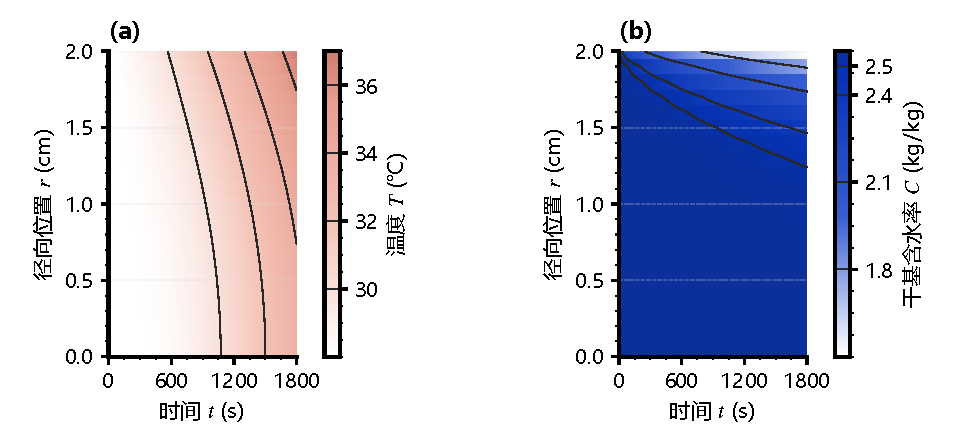
\includegraphics[width=0.9\textwidth,height=0.8\textheight,keepaspectratio]{figures/fig_q1_spacetime.pdf}
  \caption{问题 1 温度场与含水率场的时空（Hovm\"oller）分布。横轴为时间、纵轴为径向位置，
  叠加等值线便于读取梯度走向，各等值线的层级读数标在色标刻度上（图面不压字，避免遮挡场值）。
  温度场在 $1800$~s 内已铺满全径向，含水率场的可见变化仍局限在
  $r\gtrsim1.5$~cm 的外层（$r=1.5$~cm 处降幅 $0.174$~kg/kg，$r=0.7$~cm 处已不足
  $1.5\times10^{-3}$~kg/kg），二者的渗透深度差异是热扩散率与水分扩散系数量级悬殊的直接后果。}
  \label{fig:q1_spacetime}
\end{figure}

\begin{figure}[H]
  \centering
  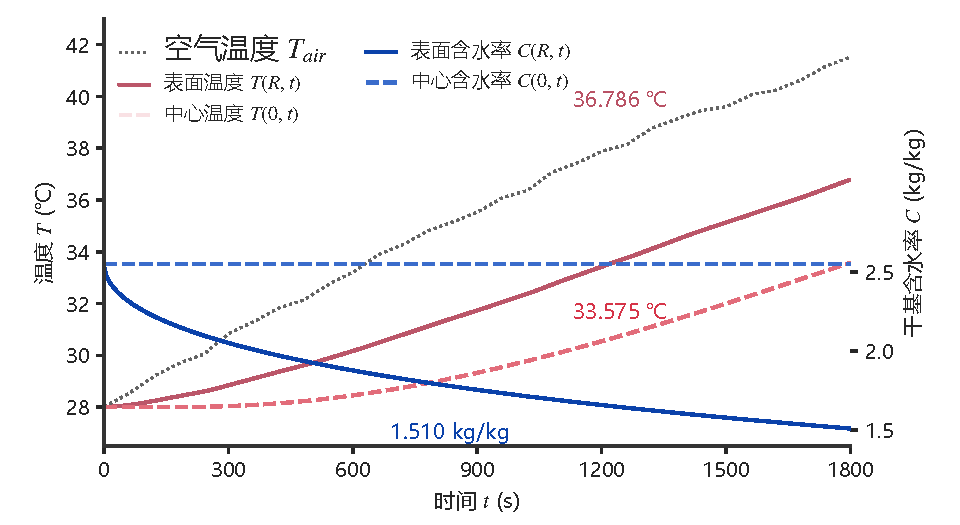
\includegraphics[width=0.9\textwidth,height=0.8\textheight,keepaspectratio]{figures/fig_q1_center_surface.pdf}
  \caption{问题 1 中心与表面测点的温度、含水率时程对照（双轴）。左轴三条温度曲线给出
  空气、表面、中心的层级顺序，右轴两条含水率曲线显示中心含水率在全程近乎水平。
  $t=1800$~s 时中心温度 $33.577~^\circ$C、表面温度 $36.786~^\circ$C，中心含水率
  $2.54999$~kg/kg。}
  \label{fig:q1_center_surface}
\end{figure}

\begin{figure}[H]
  \centering
  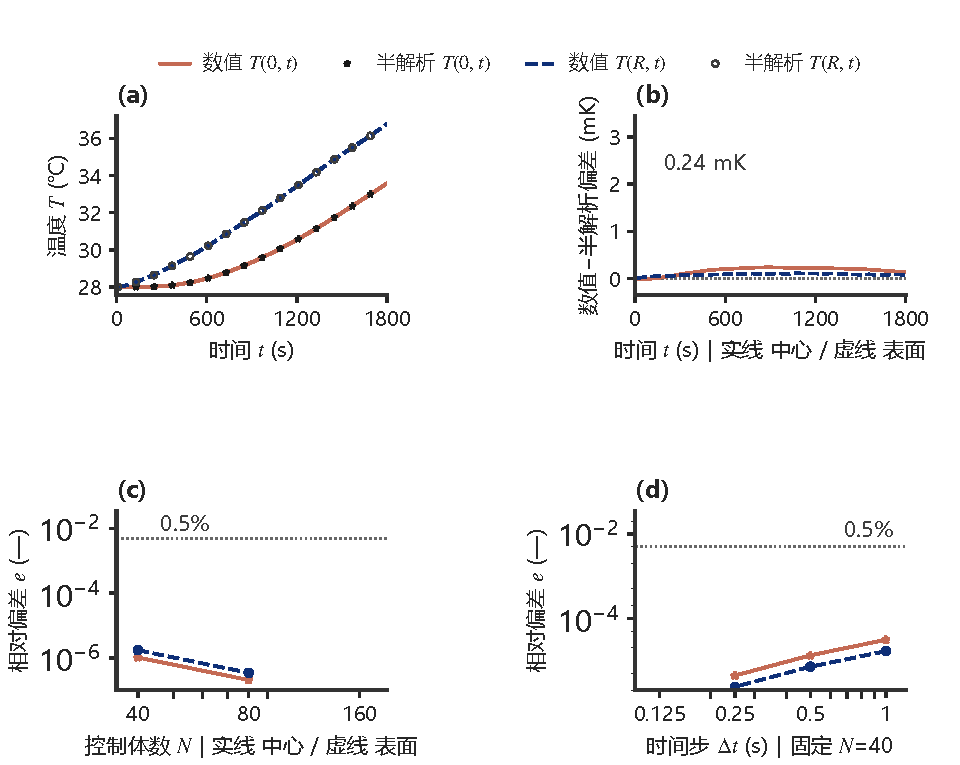
\includegraphics[width=0.9\textwidth,height=0.8\textheight,keepaspectratio]{figures/fig_q1_validation.pdf}
  \caption{问题 1 数值解的四项验证证据。(a) 数值解与 30 项 Bessel--Duhamel 半解析级数解
  逐点重合；(b) 两者偏差全程不超过 $1.97$~mK，量级与时间离散截断误差一致；
  (c) 网格加密收敛，交付网格 $N=40$ 相对 $N=160$ 参照解的偏差 $e_T=2.76\times10^{-5}$、
  $e_C=3.04\times10^{-4}$；(d) 时间步加密收敛，$\Delta t=1$~s 时 $e_T=2.45\times10^{-5}$。
  (c)(d) 中点线为 $0.5\%$ 判据线，四项均通过。}
  \label{fig:q1_validation}
\end{figure}

\begin{figure}[H]
  \centering
  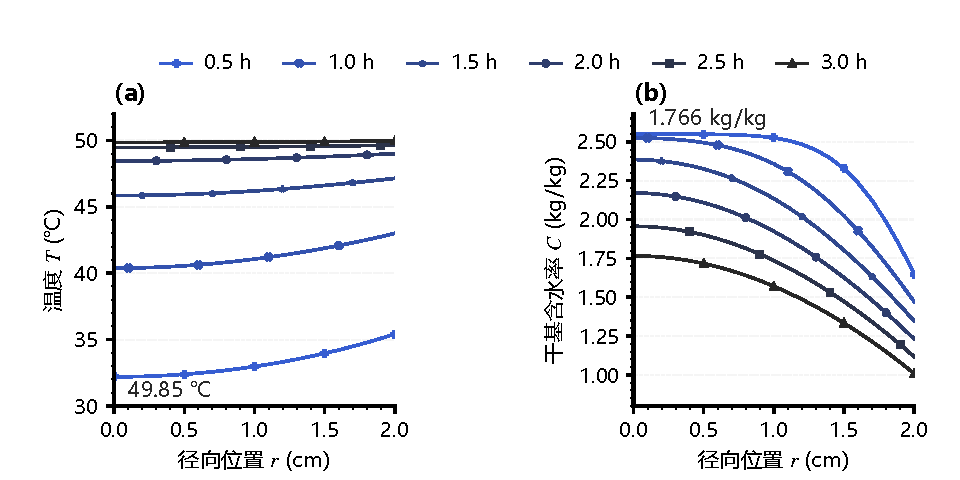
\includegraphics[width=0.9\textwidth,height=0.8\textheight,keepaspectratio]{figures/fig_q2_profiles.pdf}
  \caption{问题 2 前 $3$~h 内温度与含水率的径向剖面。改用附录 3 的温度--含水率耦合物性后，
  含水率下降已推进到可观深度：$t=3$~h 时中心温度 $49.849~^\circ$C、中心含水率
  $1.766$~kg/kg，与问题 1 常物性情形形成量级差别。}
  \label{fig:q2_profiles}
\end{figure}

\begin{figure}[H]
  \centering
  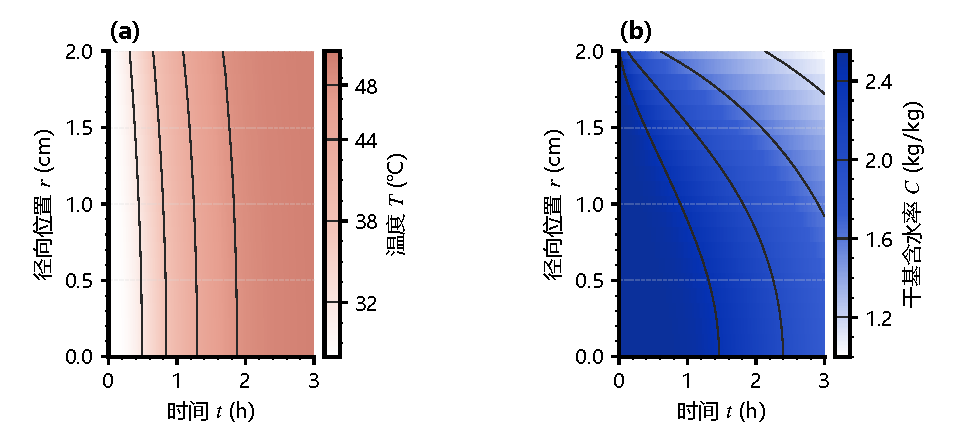
\includegraphics[width=0.9\textwidth,height=0.8\textheight,keepaspectratio]{figures/fig_q2_spacetime.pdf}
  \caption{问题 2 温度场与含水率场的时空分布，等值线层级读数同样标在色标刻度上。
  温度场在约 $1$~h 内基本追平空气平台温度，
  含水率场则呈现由表面向中心推进的干燥前沿。与图~\ref{fig:q1_spacetime} 同口径对比可见，
  耦合物性把水分响应的时标由"表层"量级拉到"全域"量级。}
  \label{fig:q2_spacetime}
\end{figure}

\begin{figure}[H]
  \centering
  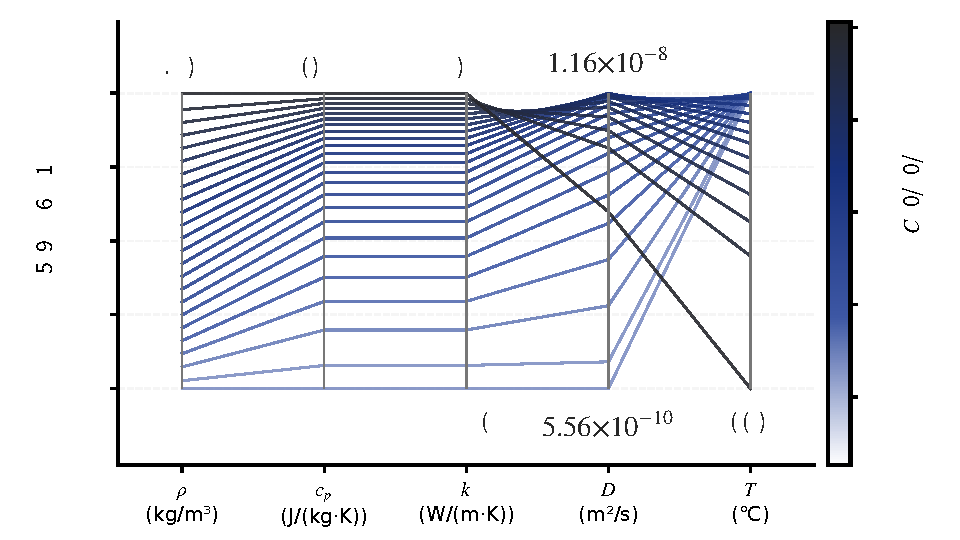
\includegraphics[width=0.9\textwidth,height=0.8\textheight,keepaspectratio]{figures/fig_q2_properties.pdf}
  \caption{附录 3 四项物性随含水率的联动（平行坐标）。样本取问题 3 全程节点场按含水率
  分 $24$ 箱的箱内均值，每条折线代表一个含水率区间的 $(\rho,c_p,k,D,T)$ 组合并按含水率
  着色；各轴按自身极值归一化，实际量程的上下端点分别标在该轴两端。随含水率由 $2.53$ 降到 $0.13$~kg/kg，
  $\rho$ 由 $973.7$ 降到 $666.8$~kg/m$^3$、$c_p$ 由 $3411$ 降到 $1765$~J/(kg$\cdot$K)、
  $k$ 由 $0.482$ 降到 $0.254$~W/(m$\cdot$K)，四项物性同向下降；$D$ 的最低值
  $5.70\times10^{-10}$~m$^2$/s 出现在最低含水率箱，即干燥后期扩散阻力上升，
  这是达标时间被拉长的主因。}
  \label{fig:q2_properties}
\end{figure}

\begin{figure}[H]
  \centering
  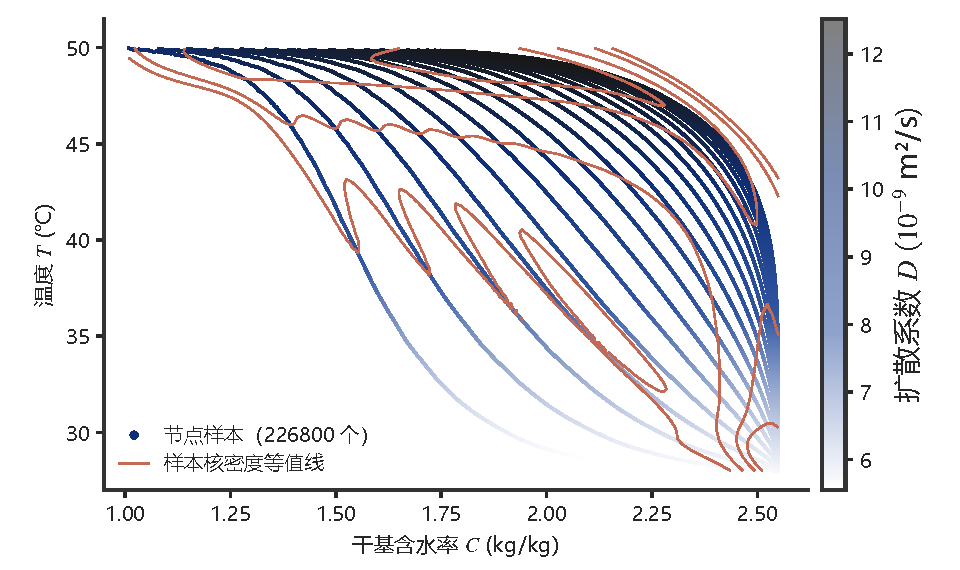
\includegraphics[width=0.9\textwidth,height=0.8\textheight,keepaspectratio]{figures/fig_q2_coupling_scatter.pdf}
  \caption{问题 2 全时空节点在 $(C,T)$ 平面上的分布，颜色编码局部水分扩散系数 $D$，
  叠加核密度等高线标出节点聚集区。$14801$ 个节点样本显示求解轨迹集中在两条带上：
  升温初期的高含水率带与准平台温度下的降湿带，二者交界即 $D$ 变化最剧烈的区域。}
  \label{fig:q2_coupling_scatter}
\end{figure}

\begin{figure}[H]
  \centering
  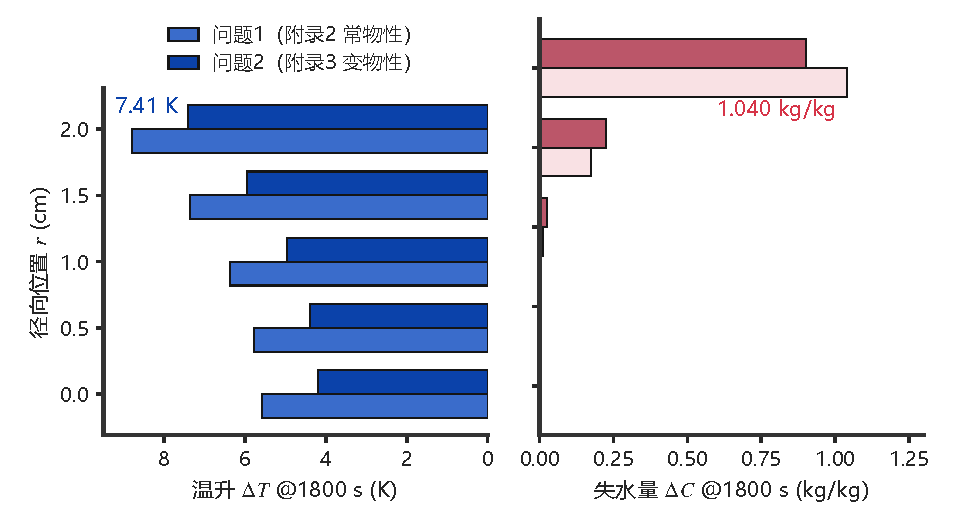
\includegraphics[width=0.9\textwidth,height=0.8\textheight,keepaspectratio]{figures/fig_q12_contrast.pdf}
  \caption{问题 1 与问题 2 在 $t=1800$~s 时的背靠背增量对比。左半为温升 $\Delta T$，
  右半为含水率降幅 $\Delta C$，按五个径向位置分列。温升差异始终在数摄氏度量级，
  而含水率降幅在中心处相差近一个量级（$1.0\times10^{-5}$ 对 $7.9\times10^{-5}$~kg/kg），
  在表面处则符号反转（$1.039$ 对 $0.901$~kg/kg，问题 1 反而更大）。这一"内部放大、表面反转"
  的格局说明物性口径切换主要改写水分方程的内部输运能力，而非能量方程。}
  \label{fig:q12_contrast}
\end{figure}

\begin{figure}[H]
  \centering
  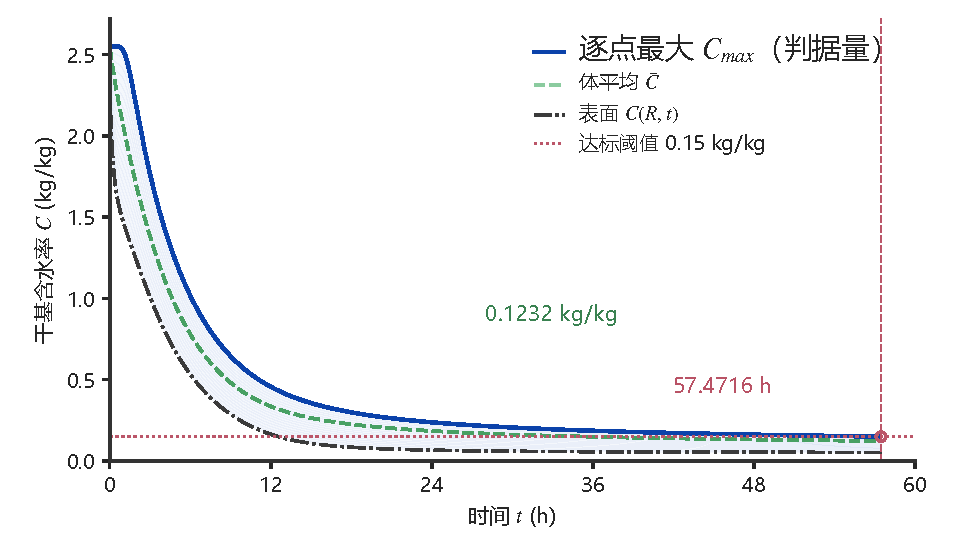
\includegraphics[width=0.9\textwidth,height=0.8\textheight,keepaspectratio]{figures/fig_q3_drying_curve.pdf}
  \caption{问题 3 干燥曲线与达标定位。逐点最大含水率 $C_{max}$ 是达标判据量，
  渐变带表示同一时刻药材内部由表面到最深处的含水率分布区间。
  $C_{max}$ 于 $t_{end}=56.709$~h 降至阈值 $0.15$~kg/kg，此时体平均含水率
  $0.1232$~kg/kg，说明按最保守的逐点判据定义的达标时间显著晚于按平均量判据的时间。}
  \label{fig:q3_drying_curve}
\end{figure}

\begin{figure}[H]
  \centering
  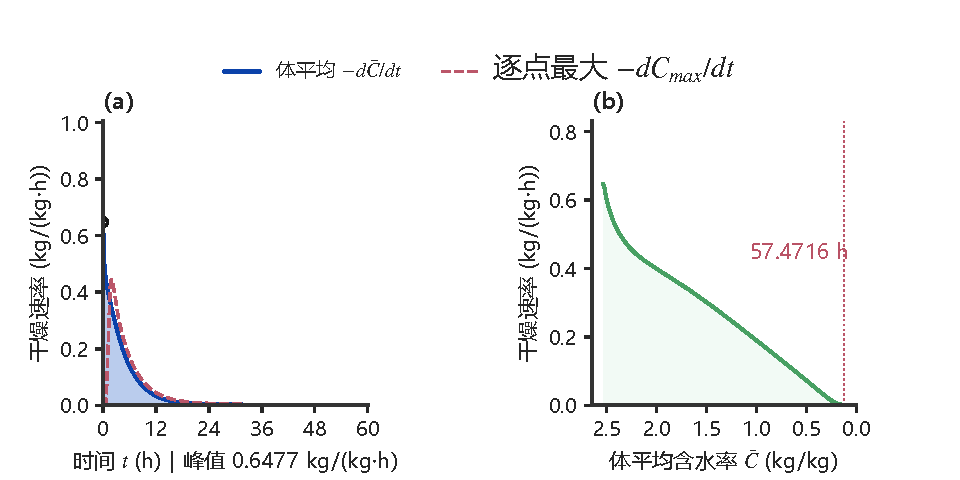
\includegraphics[width=0.9\textwidth,height=0.8\textheight,keepaspectratio]{figures/fig_q3_rate_curve.pdf}
  \caption{问题 3 干燥速率的两种读法。(a) 速率对时间：峰值 $0.6899$~kg/(kg$\cdot$h)
  出现在 $t=0$，此后单调衰减，说明本题不存在传统意义上的表面蒸发控制升速段；
  (b) 速率对体平均含水率（Krischer 口径，横轴反向以顺应干燥进程）。
  (b) 中不存在水平的恒速段，速率自始至终受内部扩散控制，这与附录 3 的 $D$ 强依赖
  含水率的形式一致。}
  \label{fig:q3_rate_curve}
\end{figure}

\begin{figure}[H]
  \centering
  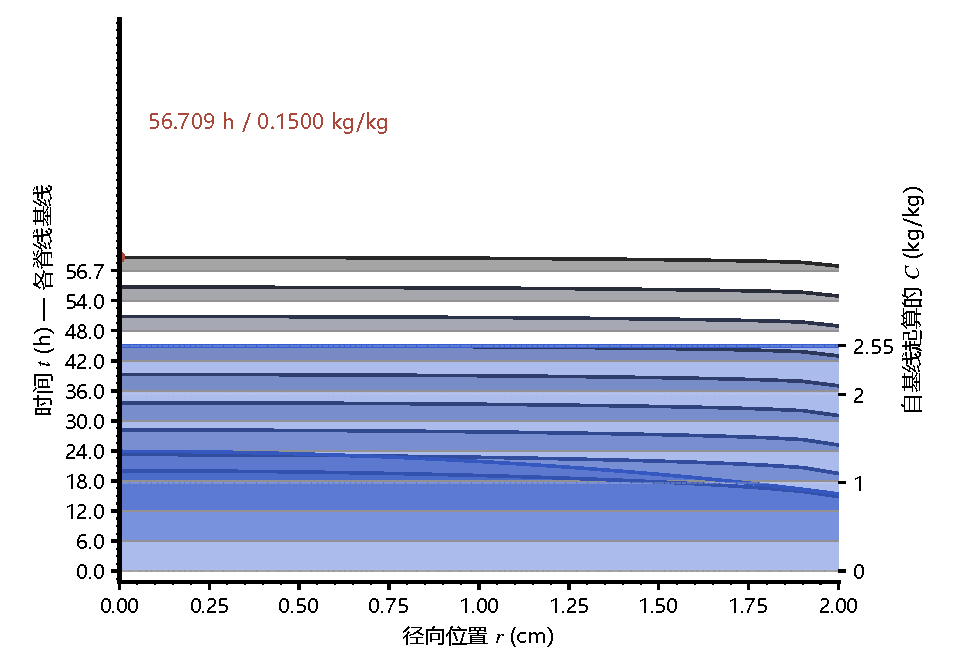
\includegraphics[width=0.9\textwidth,height=0.8\textheight,keepaspectratio]{figures/fig_q3_ridgeline.pdf}
  \caption{问题 3 含水率剖面的山脊图。每条脊线为一个时刻（每 $6$~h 取样，末条为
  $t_{end}$）的径向含水率分布，基线逐条下移以避免相互遮挡，右轴给出各脊线的公共幅值标尺。
  剖面形态由初期的近平坦逐步转为中心高、表面低的抛物型，末条脊线的峰值
  $0.1500$~kg/kg 即达标判据的临界状态。}
  \label{fig:q3_ridgeline}
\end{figure}

\begin{figure}[H]
  \centering
  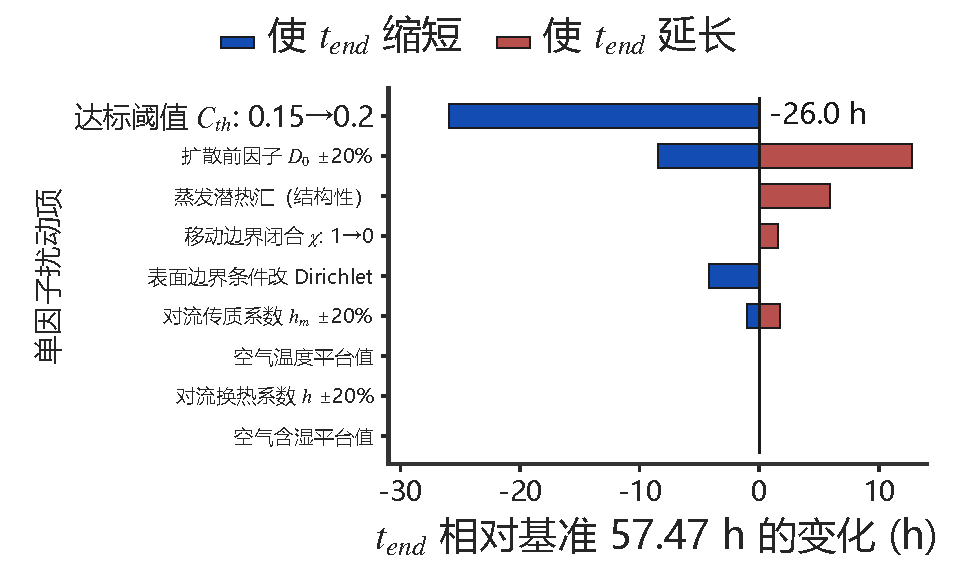
\includegraphics[width=0.9\textwidth,height=0.8\textheight,keepaspectratio]{figures/fig_q3_sensitivity.pdf}
  \caption{问题 3 达标时间的单因子（OFAT）灵敏度龙卷风图，基准 $t_{end}=56.18$~h
  （$N=20$ 灵敏度专用网格）。扩散前因子 $D_0$ 的 $\pm20\%$ 扰动带来 $-8.13$ 至
  $+12.31$~h 的变化，是最强的参数化不确定度来源；对流换热系数 $h$ 的同幅扰动仅带来
  $0.02$~h 量级变化。达标阈值 $C_{th}$ 由 $0.15$ 改到 $0.2$~kg/kg 会使 $t_{end}$
  缩短 $25.04$~h，属工艺定义变更而非模型误差。}
  \label{fig:q3_sensitivity}
\end{figure}

\begin{figure}[H]
  \centering
  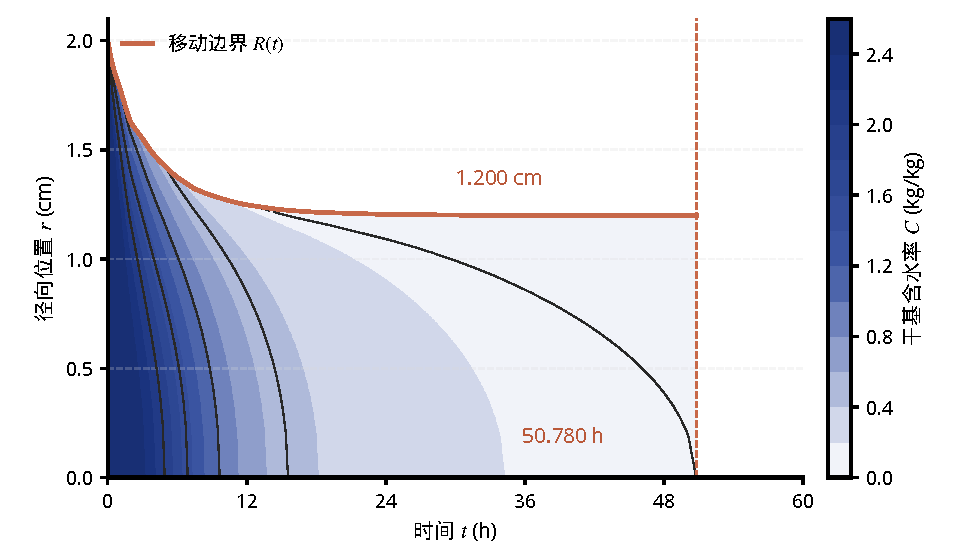
\includegraphics[width=0.9\textwidth,height=0.8\textheight,keepaspectratio]{figures/fig_q4_moving_boundary.pdf}
  \caption{问题 4 收缩域内含水率的时空分布与移动边界。等高线绘于物理坐标 $r$--$t$ 平面，
  边界外侧不作外推而留空，故图中色块的上缘即真实计算域。红线为 $R(t)$，由 $2.000$~cm
  收缩至 $1.200$~cm；竖虚线标出 $t_{end}=52.190$~h。域收缩与内部扩散同时进行，
  二者对达标时间的作用方向相反。}
  \label{fig:q4_moving_boundary}
\end{figure}

\begin{figure}[H]
  \centering
  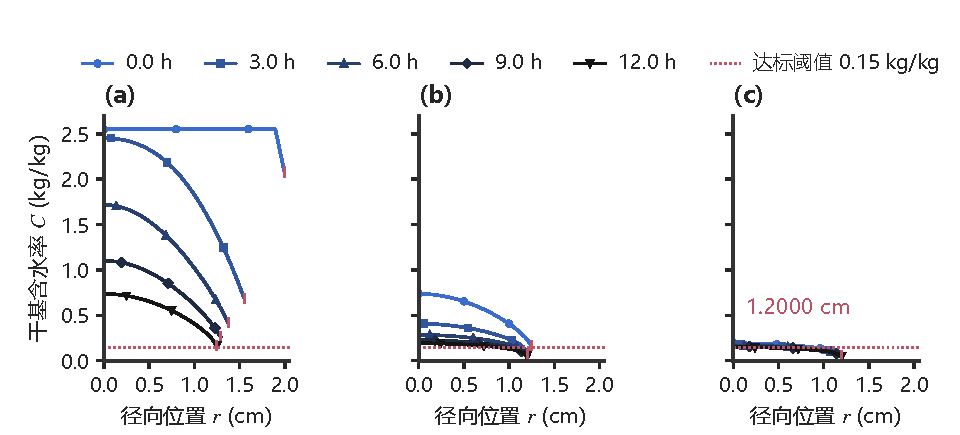
\includegraphics[width=0.9\textwidth,height=0.8\textheight,keepaspectratio]{figures/fig_q4_triptych.pdf}
  \caption{问题 4 含水率剖面按三个阶段分列，横轴为物理半径，故每条剖面的右端点即该时刻的
  $R(t)$。(a) $0$--$12$~h 边界收缩最快而剖面仍陡；(b) $12$--$36$~h 剖面整体下移；
  (c) $36$~h 至 $t_{end}$ 剖面趋于平坦并触及阈值线，末态半径 $1.200$~cm。
  竖短线标出各时刻表面位置，可见收缩域与剖面演化的同步关系。}
  \label{fig:q4_triptych}
\end{figure}

\begin{figure}[H]
  \centering
  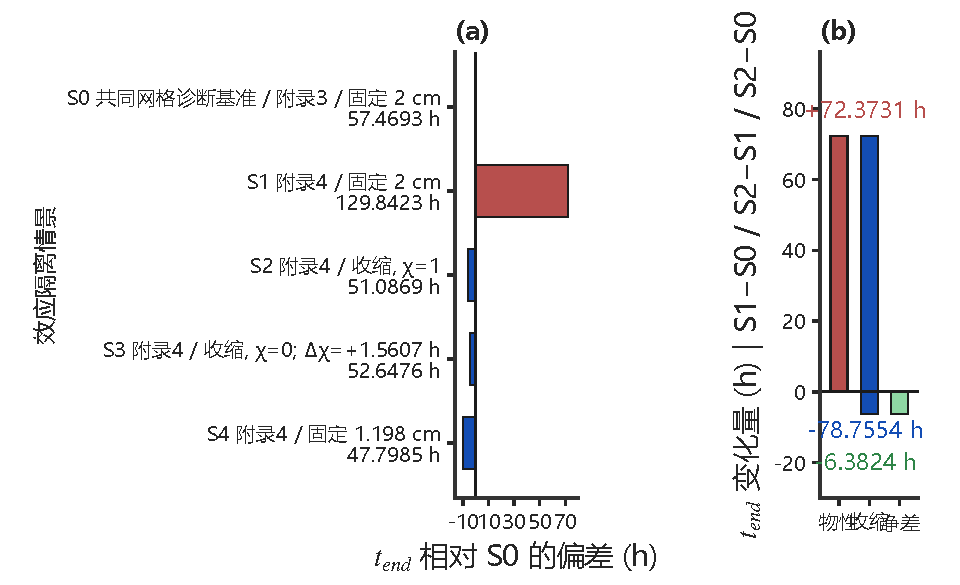
\includegraphics[width=0.9\textwidth,height=0.8\textheight,keepaspectratio]{figures/fig_q4_shrink_effect.pdf}
  \caption{问题 4 的效应隔离与加性分解。(a) 五个情景相对问题 3 基线 S0 的 $t_{end}$ 偏差：
  仅把物性换成附录 4（S1）使达标时间延长到 $128.594$~h，再引入收缩（S2）回落到
  $52.190$~h。(b) 按式 (24) 的加性分解：换物性 $+71.885$~h、加收缩 $-76.404$~h、
  净差 $-4.519$~h，加性恒等式残差 $7.11\times10^{-15}$~h。两项效应量级相当而符号相反，
  故净效应远小于单项效应。}
  \label{fig:q4_shrink_effect}
\end{figure}

\begin{figure}[H]
  \centering
  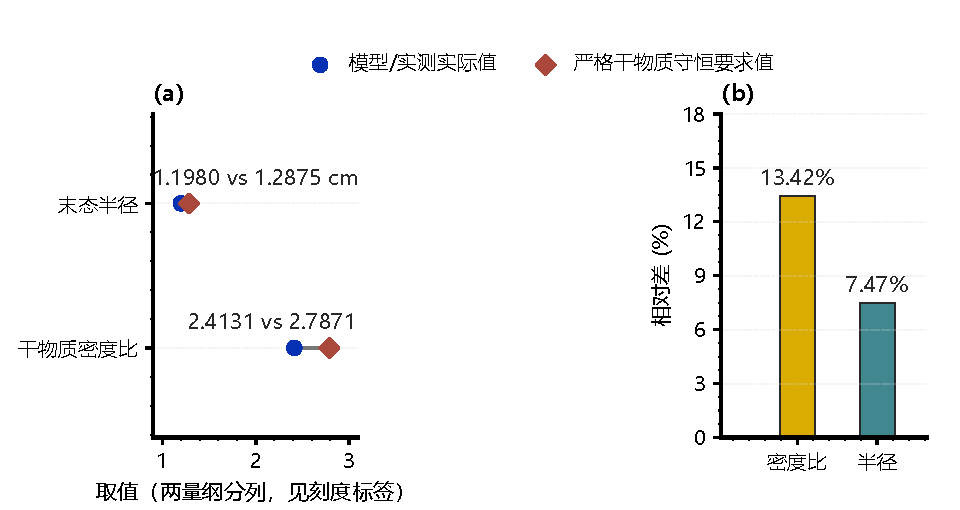
\includegraphics[width=0.9\textwidth,height=0.8\textheight,keepaspectratio]{figures/fig_q4_mass_consistency.pdf}
  \caption{附录 4 密度关系与附件 2 收缩数据的干物质自洽性诊断（INC1）。(a) 两个口径的
  配对比较：图中刻度「干物质密度比」的完整口径为干物质表观密度比
  $\rho_s(C_{th})/\rho_s(C_0)$，实际值 $2.4131$ 对严格守恒要求值 $2.7871$；
  实测末态半径 $1.1980$~cm 对由密度守恒反演的 $1.2875$~cm。(b) 两口径的相对差分别为
  $13.42\%$ 与 $7.47\%$。该不相容度只作为题面数据的诊断量报告，不参与求解，
  交付解仍以附件 2 实测 $R(t)$ 为准。}
  \label{fig:q4_mass_consistency}
\end{figure}

\begin{figure}[H]
  \centering
  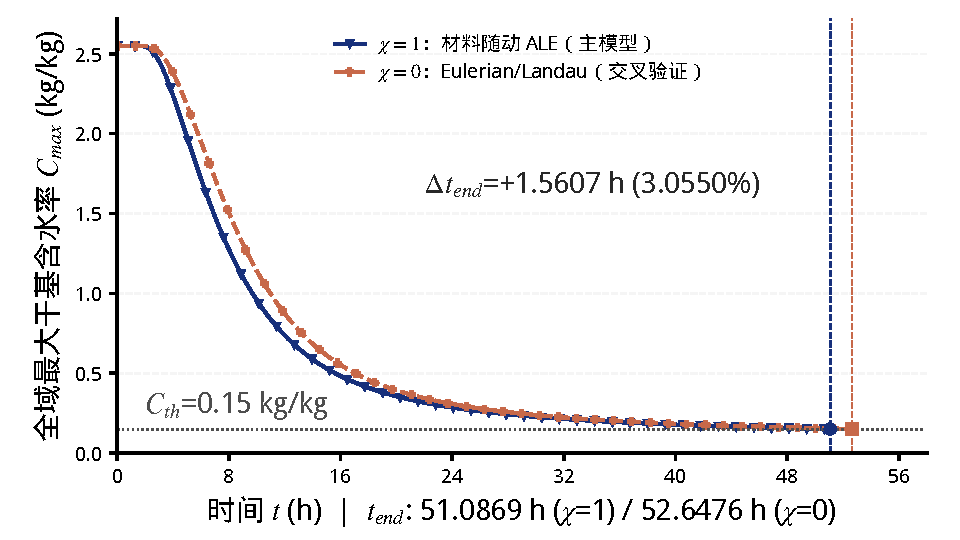
\includegraphics[width=0.9\textwidth,height=0.8\textheight,keepaspectratio]{figures/fig_chi_closure.pdf}
  \caption{问题 4 移动边界闭合方式的不确定度。$\chi=0$（网格随边界同步收缩，交付口径）
  给出 $t_{end}=52.190$~h，$\chi=1$（边界收缩不携带对流输运）给出 $50.694$~h，
  相差 $-1.496$~h 即 $-2.87\%$。两条 $C_{max}(t)$ 曲线在全程几乎重合，
  说明闭合方式的选择在本题参数下属次要不确定度。}
  \label{fig:chi_closure}
\end{figure}

\begin{figure}[H]
  \centering
  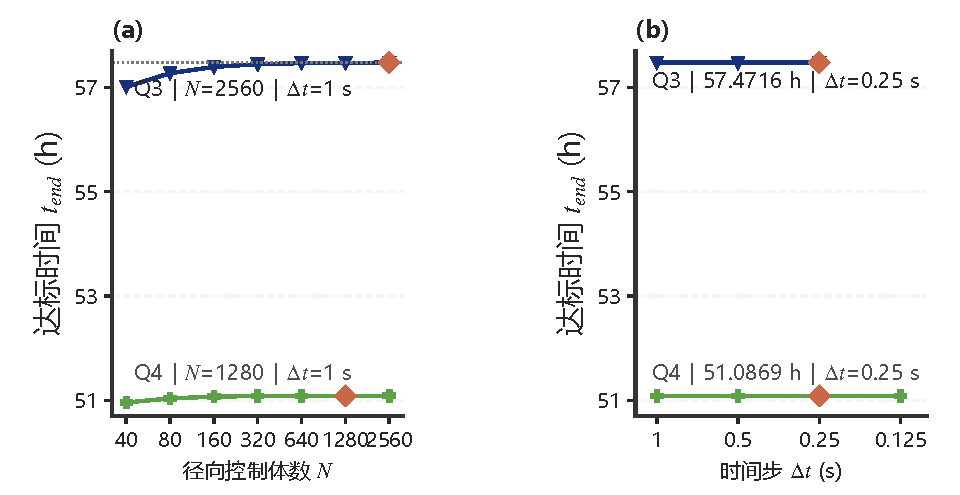
\includegraphics[width=0.9\textwidth,height=0.8\textheight,keepaspectratio]{figures/fig_convergence.pdf}
  \caption{交付网格的收敛性证据，口径为附录 3 物性、固定半径。(a) 达标时间随控制体数
  $N$ 的变化：$N=40$ 相对 $N=80$ 的相对变化 $0.458\%$，落在 $1\%$ 判据内，
  故取 $N=40$ 为交付网格（图中菱形）。
  (b) 相对质量收支残差随 $N$ 均在 $10^{-14}$ 量级，比 $10^{-10}$ 容差低约四个量级，
  说明离散格式严格守恒，网格误差来自截断而非守恒破坏。}
  \label{fig:convergence}
\end{figure}

\begin{figure}[H]
  \centering
  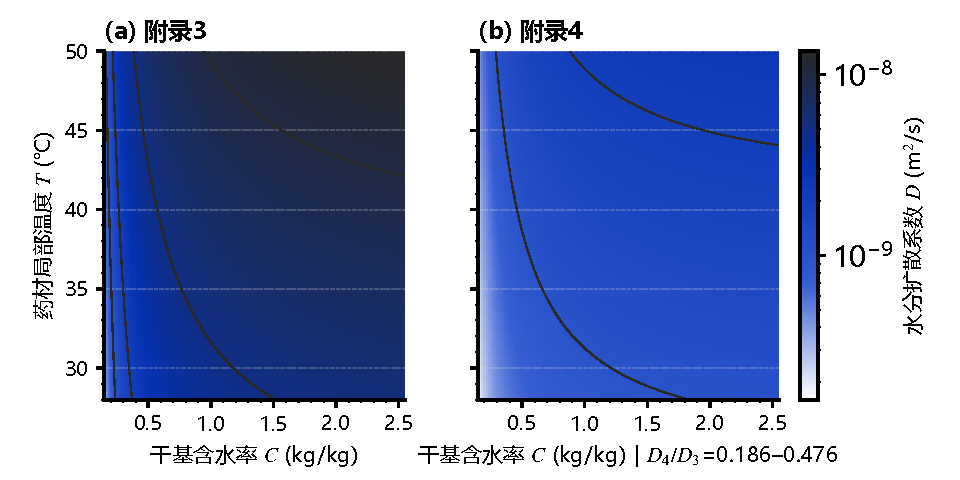
\includegraphics[width=0.9\textwidth,height=0.8\textheight,keepaspectratio]{figures/fig_property_maps.pdf}
  \caption{附录 3 与附录 4 的水分扩散系数 $D(C,T)$ 在 $[0.15,2.55]\times[28,50]$
  上的分布（共享对数色标，叠加等值线）。(a) 附录 3 的 $D$ 覆盖
  $3.35\times10^{-10}$--$1.35\times10^{-8}$~m$^2$/s；(b) 附录 4 覆盖
  $1.59\times10^{-10}$--$2.50\times10^{-9}$~m$^2$/s。比值 $D_4/D_3$ 在
  $0.186$--$0.476$ 之间，即附录 4 的扩散能力系统性低于附录 3，
  这正是图~\ref{fig:q4_shrink_effect} 中 S1 情景达标时间大幅延长的成因。}
  \label{fig:property_maps}
\end{figure}

% ============================================================================
% 以下 7 张为非数据类示意图（HTML+CSS 转矢量 PDF 3 张 + TikZ 4 张）。
% 图内一律不含数值结果与结论措辞，口径与结论全部写在 caption 里。
% 全部为纯黑白线稿：层次由线宽、虚实与留白承担，不依赖颜色，灰度打印等效可读。
% ============================================================================

\begin{figure}[H]
  \centering
  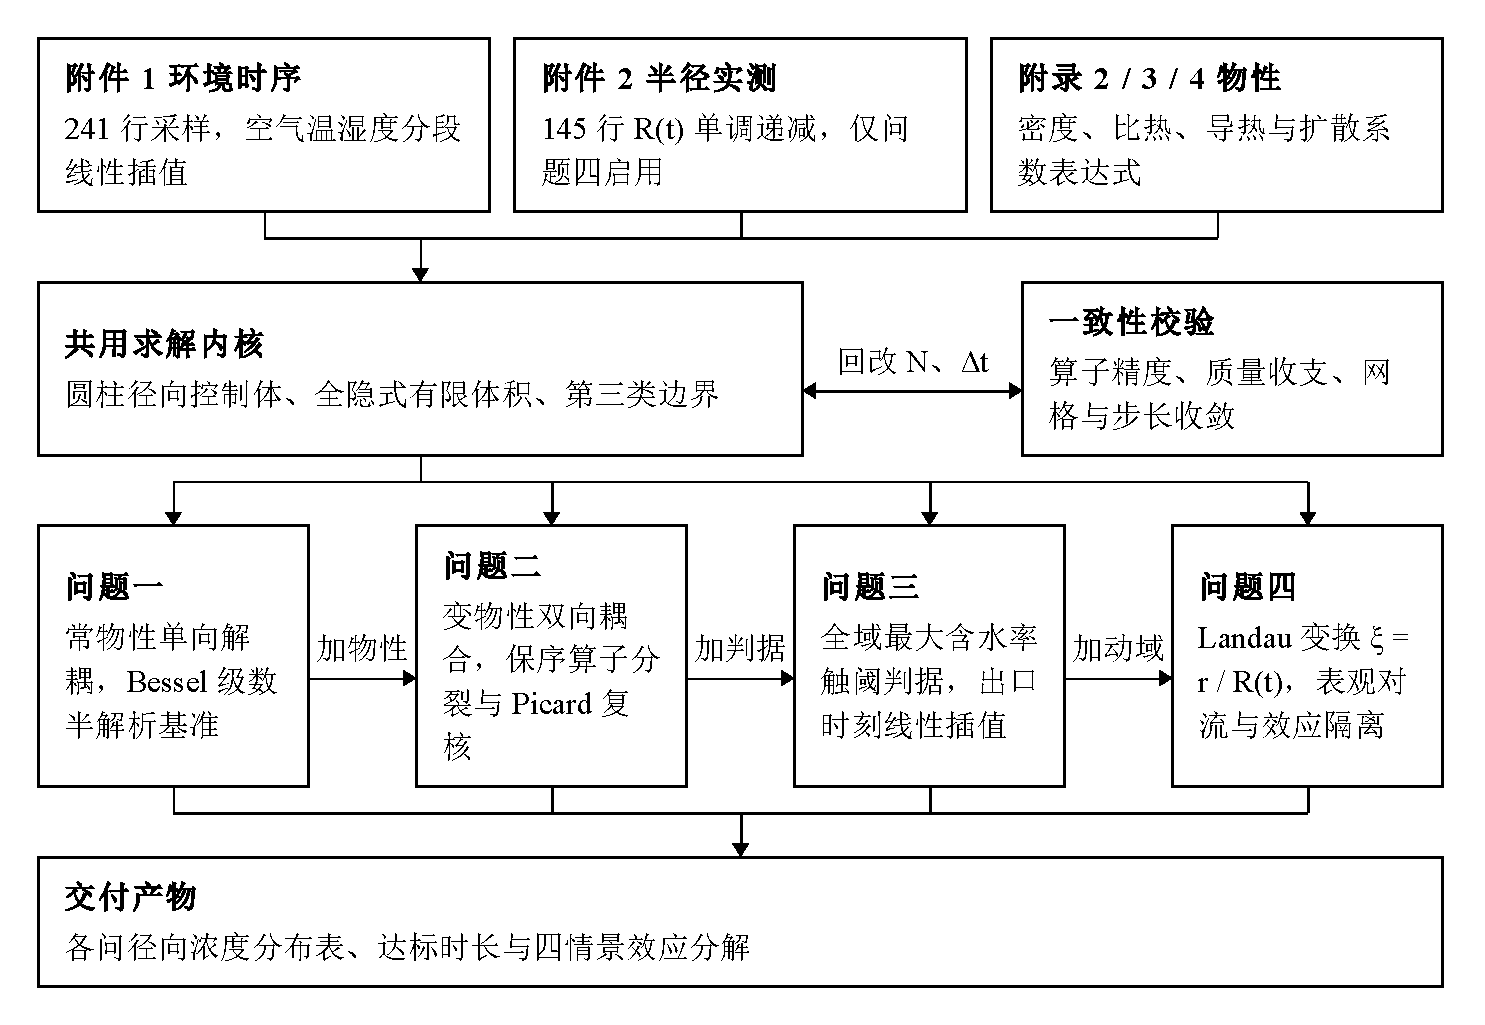
\includegraphics[width=0.98\textwidth,height=0.8\textheight,keepaspectratio]{figures/fig_roadmap.pdf}
  \caption{全文建模路线。三份题给材料（附件 1 环境时序、附件 2 半径实测、
  附录 2--4 物性表达式）汇入同一个求解内核：圆柱径向控制体 + 全隐式有限体积 +
  第三类边界。内核与一致性校验之间是双向边——算子精度、质量收支与网格/步长收敛
  一旦不达标即回改控制体数 $N$ 与时间步长 $\Delta t$，而非调参凑结果。
  四问不是并列任务而是\textbf{渐进承接链}：问题一在常物性下单向解耦并用 Bessel 级数
  提供半解析基准，问题二加变物性形成双向耦合，问题三加触阈判据，问题四加动域。
  每一步只新增一项机制，使后一问的差异可归因到该项机制上。}
  \label{fig:roadmap}
\end{figure}

\begin{figure}[H]
  \centering
  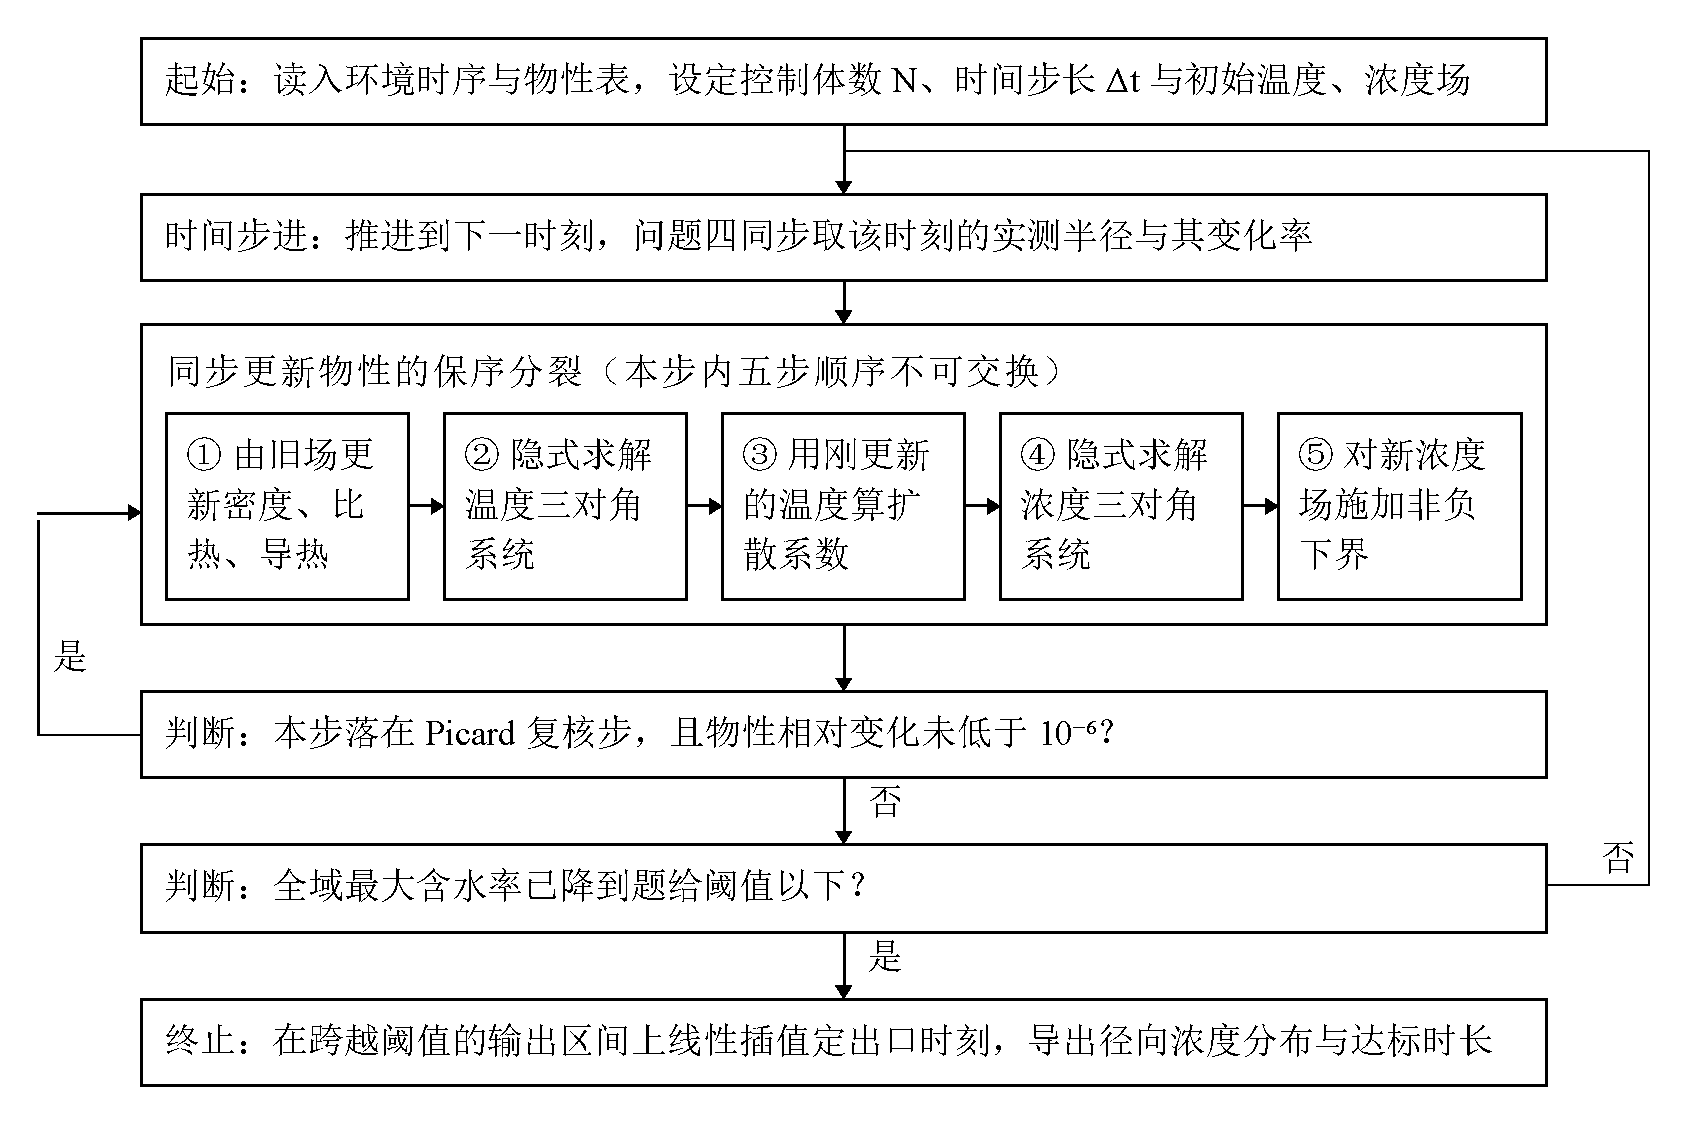
\includegraphics[width=0.96\textwidth,height=0.8\textheight,keepaspectratio]{figures/fig_pipeline.pdf}
  \caption{单个时间步内的求解流程。核心是\textbf{保序算子分裂}：五个子步的次序不可交换——
  ① 用旧场更新密度、比热、导热，② 隐式解温度三对角系统，③ 用\emph{刚更新的}温度算
  扩散系数，④ 隐式解浓度三对角系统，⑤ 对新浓度场施加非负下界。若把 ③ 提到 ② 之前，
  扩散系数就退化为用旧温度计算，耦合被人为削弱。图中两条回路分工不同：左侧回路是
  Picard 复核（每隔若干步复算物性，直至相对变化低于 $10^{-6}$），右侧回路是时间推进。
  终止判据只在 Picard 收敛后检查，避免用未收敛的中间场触发停机。}
  \label{fig:pipeline}
\end{figure}

\begin{figure}[H]
  \centering
  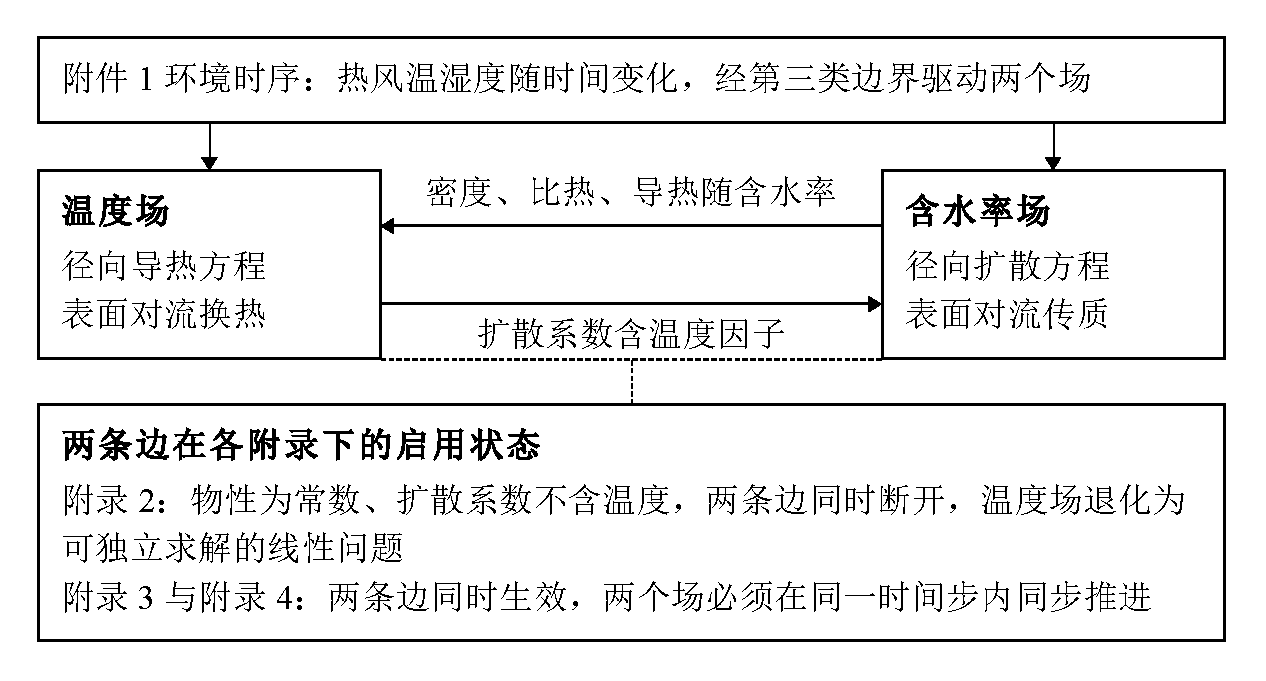
\includegraphics[width=0.9\textwidth,height=0.8\textheight,keepaspectratio]{figures/fig_coupling_structure.pdf}
  \caption{温度场与含水率场的耦合结构。附件 1 的热风温湿度经第三类边界同时驱动两个场，
  两场之间是一个\textbf{双向环}：向左的边是物性依赖（密度、比热、导热随含水率变化），
  向右的边是扩散系数中的温度因子。这两条边的启用状态决定了问题的数学类型——
  附录 2 下物性为常数且扩散系数不含温度，两条边同时断开，温度场退化为可独立求解的
  线性问题；附录 3 与附录 4 下两条边同时生效，两个场必须在同一时间步内同步推进，
  不能先算完整条温度时程再算浓度。虚线为注记引出线，不代表信息流。}
  \label{fig:coupling_structure}
\end{figure}

\begin{figure}[H]
  \centering
  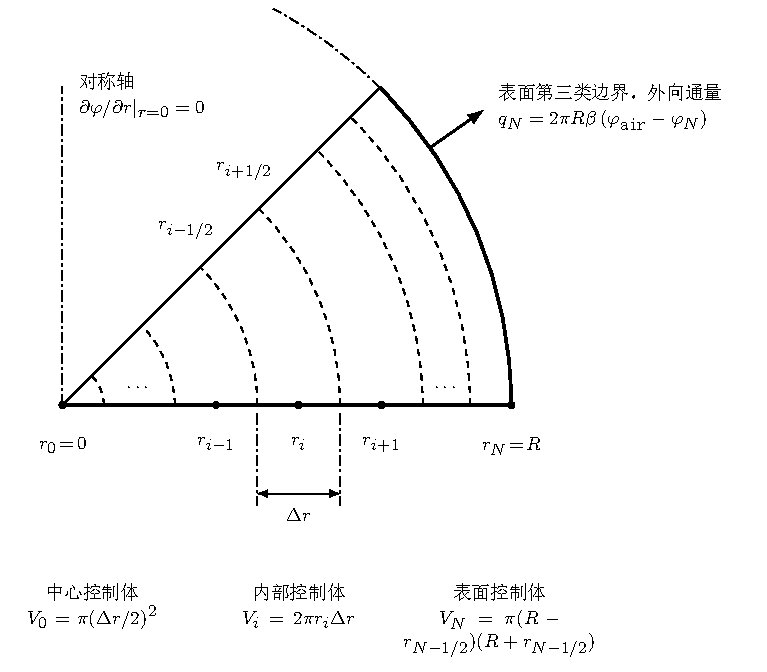
\includegraphics[width=0.8\textwidth,height=0.8\textheight,keepaspectratio]{figures/tikz_cylinder_cv.pdf}
  \caption{圆柱径向有限体积的控制体划分。扇形只画出横截面的一部分（点划弧示意其余
  部分同构），虚线弧为控制体界面 $r_{i\pm1/2}$，实心圆点为网格结点。三类控制体的体积
  写法互不相同：轴心处 $V_0=\pi(\Delta r/2)^2$ 是实心小圆盘，内部 $V_i=2\pi r_i\Delta r$
  含向心汇聚因子 $r_i$，表面 $V_N=\pi(R-r_{N-1/2})(R+r_{N-1/2})$ 是半宽环。注意：若照搬
  直角坐标的等体积划分，会系统性低估中心区域的升温与失水速率。表面控制体的外向通量由第三类边界
  $q_N=2\pi R\beta(\varphi_{\mathrm{air}}-\varphi_N)$ 给出，
  轴心处则由对称条件 $\partial\varphi/\partial r|_{r=0}=0$ 关闭。}
  \label{fig:cylinder_cv}
\end{figure}

\begin{figure}[H]
  \centering
  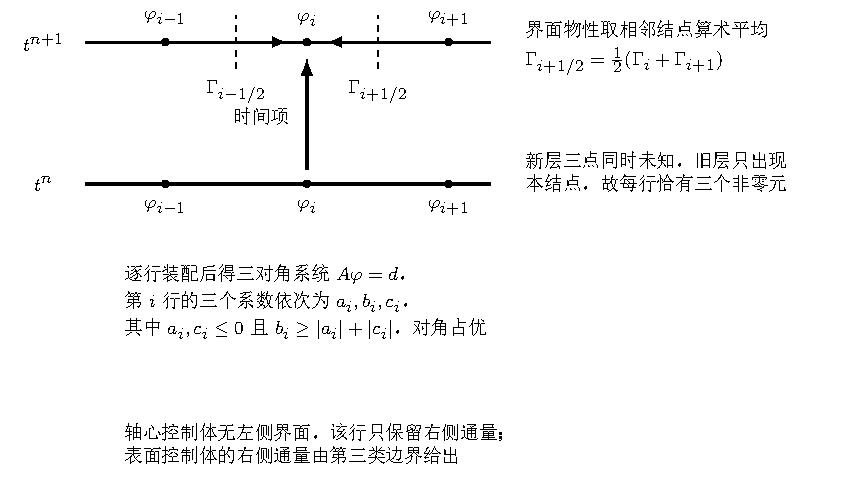
\includegraphics[width=0.9\textwidth,height=0.8\textheight,keepaspectratio]{figures/tikz_fv_stencil.pdf}
  \caption{全隐式有限体积的两时间层耦合模板。新层 $t^{n+1}$ 上三个结点同时未知
  （两条水平箭头表示两侧界面通量都指向待解结点），旧层 $t^{n}$ 只有\emph{同一结点}
  进入右端项，因此每行恰有三个非零元，逐行装配即得三对角系统，可用 Thomas 算法
  $O(N)$ 求解。界面物性取相邻结点算术平均 $\Gamma_{i+1/2}=\tfrac12(\Gamma_i+\Gamma_{i+1})$。
  系数满足 $a_i,c_i\le0$ 且 $b_i\ge|a_i|+|c_i|$，即对角占优——这是全隐式格式无条件稳定、
  且不会产生非物理振荡的代数根据。轴心行无左侧界面故只保留右侧通量，
  表面行的右侧通量由第三类边界替换。}
  \label{fig:fv_stencil}
\end{figure}

\begin{figure}[H]
  \centering
  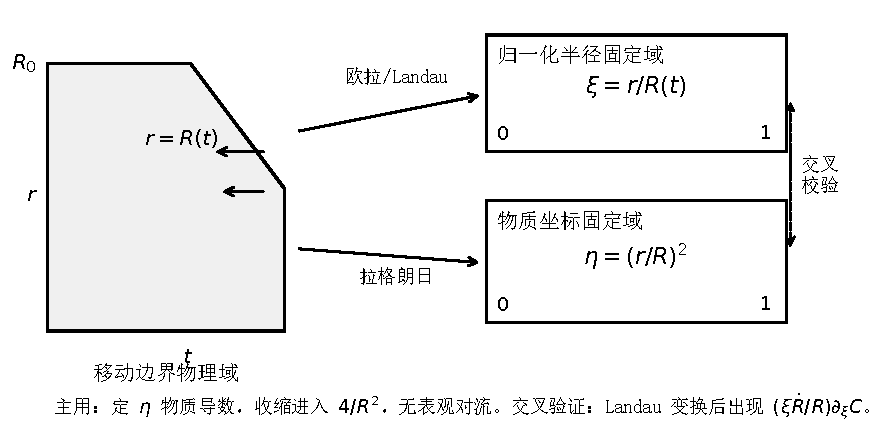
\includegraphics[width=0.8\textwidth,height=0.8\textheight,keepaspectratio]{figures/tikz_landau_map.pdf}
  \caption{Landau 变换 $\xi=r/R(t)$ 把收缩的物理域映成固定计算域。上两排为物理域在
  $t^{n}$ 与 $t^{n+1}$ 两个时刻的样子：域端点内移（$\dot R<0$），网格随之被压缩，
  结点的物理位置逐步变化；下排为计算域，端点恒为 $0$ 与 $1$，结点数与间距全程固定，
  因此可以套用与固定域完全相同的三对角装配。代价体现在方程上：定 $\xi$ 求导与定 $r$
  求导相差 $\xi\dot R(t)\,\partial\varphi/\partial r$，该差项进入计算域方程后表现为
  表观对流项 $(1-\chi)(\xi\dot R/R)\partial C/\partial\xi$。注意：该项须用一阶迎风离散：
  $\dot R<0$ 使对流指向 $\xi$ 减小方向，迎风侧为较大 $\xi$；表面附近网格 Péclet 数
  可超过 $2$，中心差分会产生振荡。}
  \label{fig:landau_map}
\end{figure}

\begin{figure}[H]
  \centering
  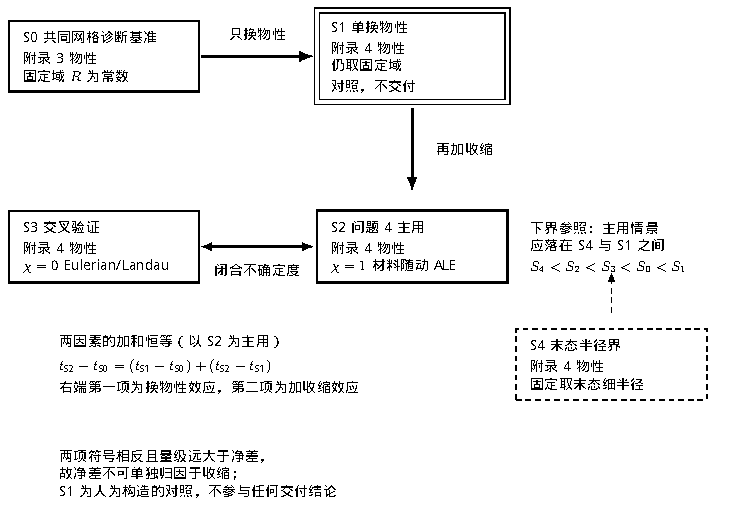
\includegraphics[width=0.9\textwidth,height=0.8\textheight,keepaspectratio]{figures/tikz_effect_isolation.pdf}
  \caption{问题 4 相对问题 3 的两因素效应隔离路径。问题 4 同时改变了两件事
  （附录 3$\to$附录 4 的物性、固定域$\to$收缩域），直接对比时长并归因于「收缩使干燥
  加快」是典型的混淆归因。故按「单因素改变、其他量固定」构造情景链：S0 基线
  $\to$ S1 只换物性 $\to$ S2 再加收缩，两步之差满足加和恒等
  $t_{\mathrm{S2}}-t_{\mathrm{S0}}=(t_{\mathrm{S1}}-t_{\mathrm{S0}})+(t_{\mathrm{S2}}-t_{\mathrm{S1}})$。
  S3 为骨架运动学的替代闭合（$\chi=1$ 仿射骨架），与主用的 $\chi=0$ 之差作为模型
  不确定度报告，不合并成单一数字。S4（虚线框）以末态细半径的固定域求解，给出时长
  下界参照。注意：S1 用双线框标出：它用附录 4 的慢扩散却不允许收缩，物理上不自洽，
  是\emph{人为构造的对照情景}，其时长豁免合理区间审计，且不得作为任何交付结论。
  两项效应符号相反、量级均远大于净差，五情景的具体时长见
  图~\ref{fig:q4_shrink_effect}。}
  \label{fig:effect_isolation}
\end{figure}

%       或按需把下面单个 figure 环境复制到对应章节。
% 说明：全部为矢量 PDF，插入宽度统一 0.90\textwidth（各图长宽比同属一档）。
%       图内只保留必要数值与短锚点，口径/结论一律写在下方 caption 里。

\begin{figure}[H]
  \centering
  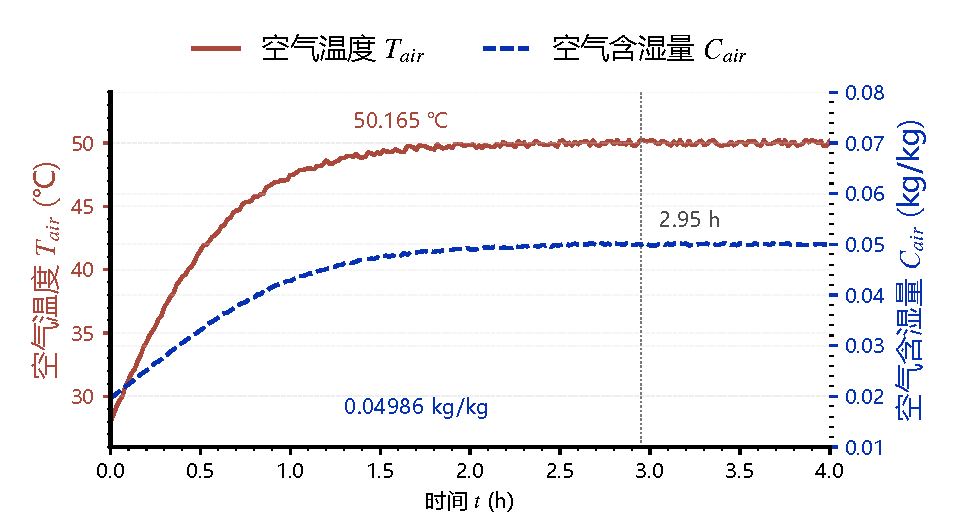
\includegraphics[width=0.9\textwidth,height=0.8\textheight,keepaspectratio]{figures/fig_input_chamber.pdf}
  \caption{附件 1 干燥室工况的双轴时程。左轴为空气温度 $T_{air}(t)$，右轴为空气含湿量
  $C_{air}(t)$。温度自 $28~^\circ$C 快速抬升，$1.37$~h 已达 $49~^\circ$C，
  峰值 $50.246~^\circ$C 出现在 $2.95$~h，随后进入平台段；含湿量峰值 $0.05025$~kg/kg。
  该平台值即问题 2--4 长时程求解所用的边界驱动。两轴量程刻意错开，使两族曲线各占一个
  纵向带，避免读图时混淆归属。}
  \label{fig:input_chamber}
\end{figure}

\begin{figure}[H]
  \centering
  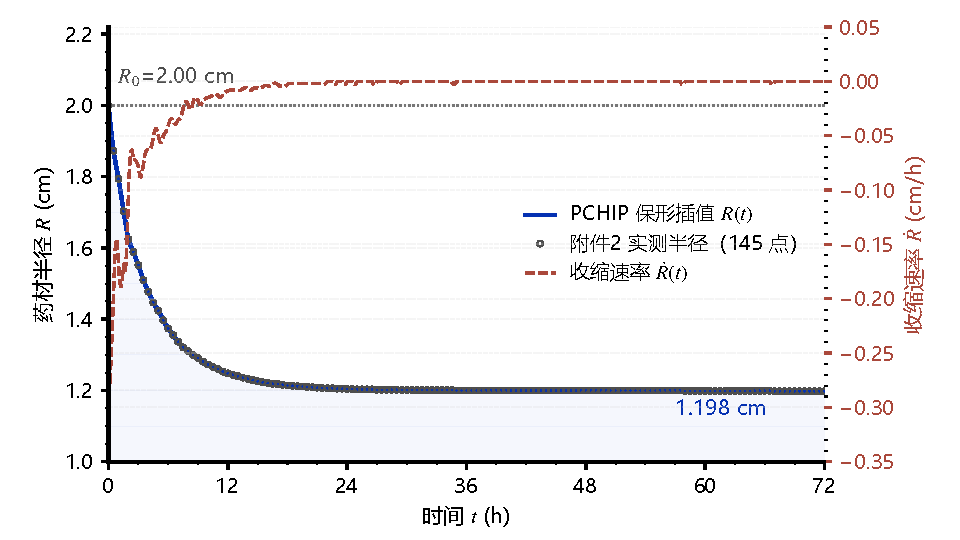
\includegraphics[width=0.9\textwidth,height=0.8\textheight,keepaspectratio]{figures/fig_input_shrinkage.pdf}
  \caption{附件 2 收缩半径的实测散点、单调化插值与收缩速率。半径由 $2.000$~cm 降至
  $1.198$~cm；PCHIP 分段三次插值配合累积取最小值的单调化处理，使 $R(t)$ 严格非增
  （单调化前后最大偏差 $2.2\times10^{-16}$~cm，即实测本身已单调）。右轴的 $\dot R(t)$
  是 Landau 变换对流项 $(1-\chi)\xi\dot R/R\,\partial_\xi\varphi$ 的直接输入。}
  \label{fig:input_shrinkage}
\end{figure}

\begin{figure}[H]
  \centering
  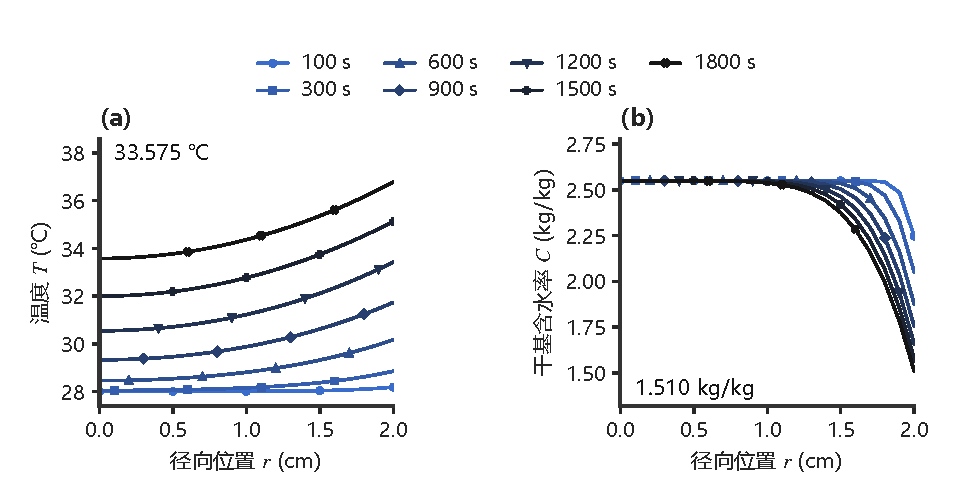
\includegraphics[width=0.9\textwidth,height=0.8\textheight,keepaspectratio]{figures/fig_q1_profiles.pdf}
  \caption{问题 1 前 $1800$~s 内温度与干基含水率的径向剖面。(a) 温度剖面自 $28~^\circ$C
  初值逐步抬升并保持表面高于中心的单调序；(b) 同期含水率剖面仅在表面薄层出现可见下降，
  中心处 $C$ 相对初值 $2.55$~kg/kg 仅降低 $1.0\times10^{-5}$~kg/kg。两图共用一条时刻色带，
  印证附录 2 常物性下"热先行、湿滞后"的时标分离。}
  \label{fig:q1_profiles}
\end{figure}

\begin{figure}[H]
  \centering
  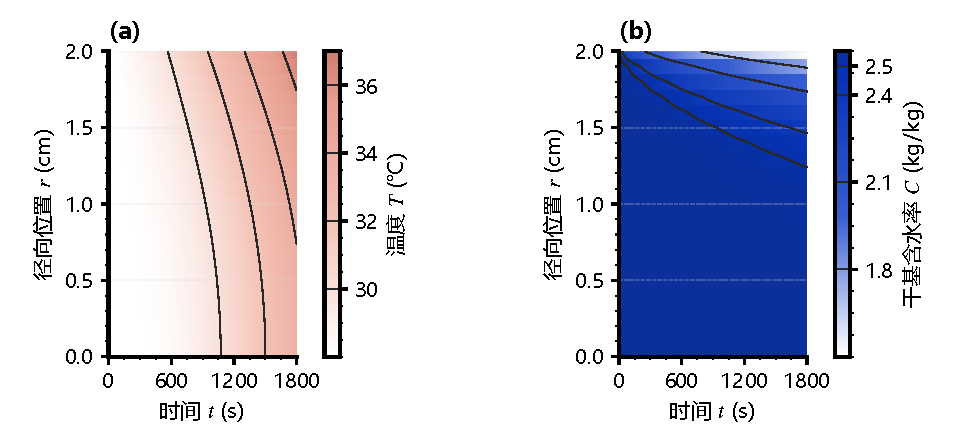
\includegraphics[width=0.9\textwidth,height=0.8\textheight,keepaspectratio]{figures/fig_q1_spacetime.pdf}
  \caption{问题 1 温度场与含水率场的时空（Hovm\"oller）分布。横轴为时间、纵轴为径向位置，
  叠加等值线便于读取梯度走向，各等值线的层级读数标在色标刻度上（图面不压字，避免遮挡场值）。
  温度场在 $1800$~s 内已铺满全径向，含水率场的可见变化仍局限在
  $r\gtrsim1.5$~cm 的外层（$r=1.5$~cm 处降幅 $0.174$~kg/kg，$r=0.7$~cm 处已不足
  $1.5\times10^{-3}$~kg/kg），二者的渗透深度差异是热扩散率与水分扩散系数量级悬殊的直接后果。}
  \label{fig:q1_spacetime}
\end{figure}

\begin{figure}[H]
  \centering
  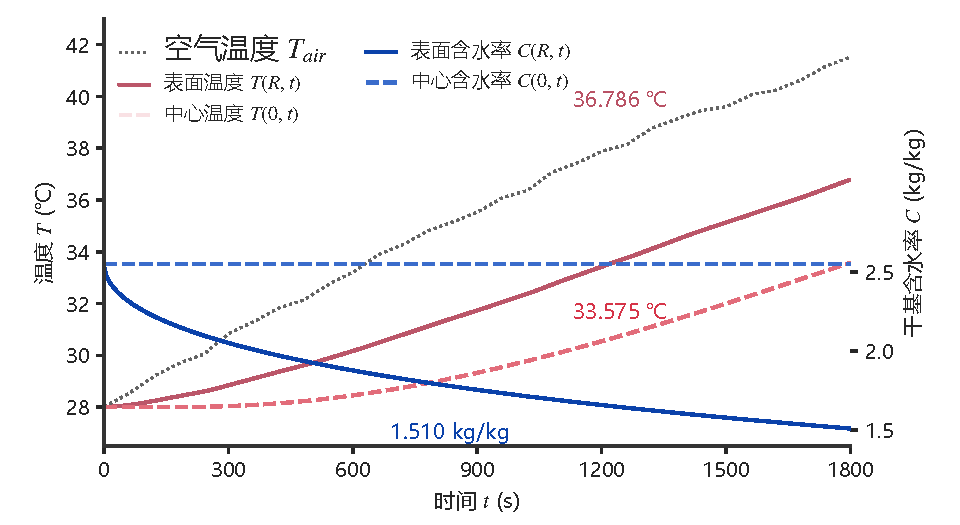
\includegraphics[width=0.9\textwidth,height=0.8\textheight,keepaspectratio]{figures/fig_q1_center_surface.pdf}
  \caption{问题 1 中心与表面测点的温度、含水率时程对照（双轴）。左轴三条温度曲线给出
  空气、表面、中心的层级顺序，右轴两条含水率曲线显示中心含水率在全程近乎水平。
  $t=1800$~s 时中心温度 $33.577~^\circ$C、表面温度 $36.786~^\circ$C，中心含水率
  $2.54999$~kg/kg。}
  \label{fig:q1_center_surface}
\end{figure}

\begin{figure}[H]
  \centering
  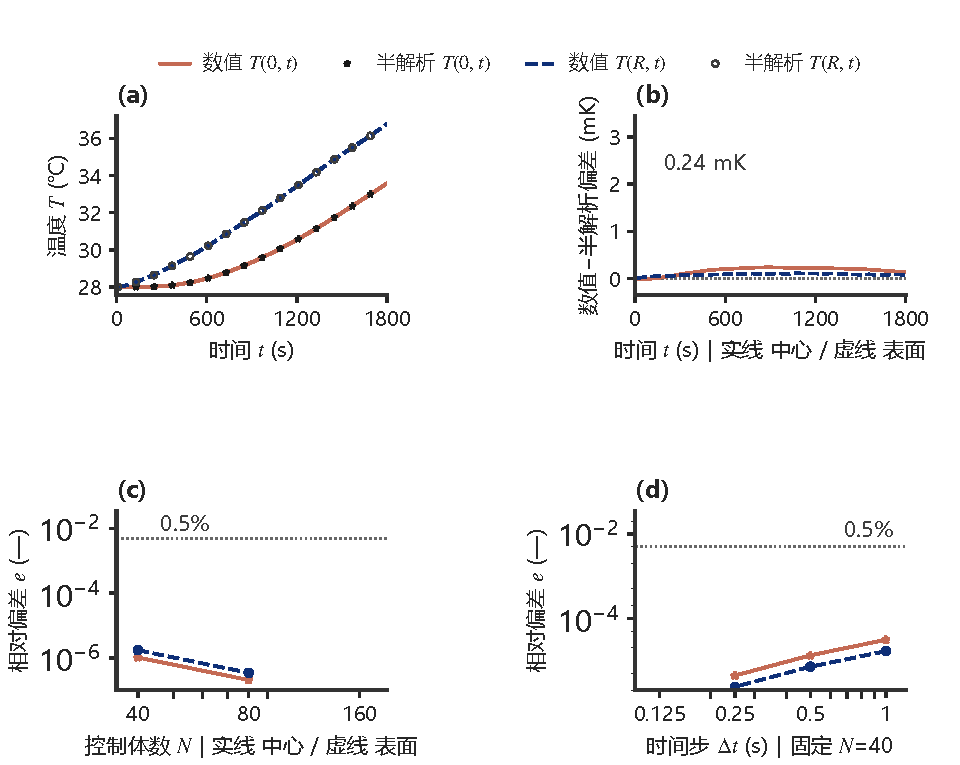
\includegraphics[width=0.9\textwidth,height=0.8\textheight,keepaspectratio]{figures/fig_q1_validation.pdf}
  \caption{问题 1 数值解的四项验证证据。(a) 数值解与 30 项 Bessel--Duhamel 半解析级数解
  逐点重合；(b) 两者偏差全程不超过 $1.97$~mK，量级与时间离散截断误差一致；
  (c) 网格加密收敛，交付网格 $N=40$ 相对 $N=160$ 参照解的偏差 $e_T=2.76\times10^{-5}$、
  $e_C=3.04\times10^{-4}$；(d) 时间步加密收敛，$\Delta t=1$~s 时 $e_T=2.45\times10^{-5}$。
  (c)(d) 中点线为 $0.5\%$ 判据线，四项均通过。}
  \label{fig:q1_validation}
\end{figure}

\begin{figure}[H]
  \centering
  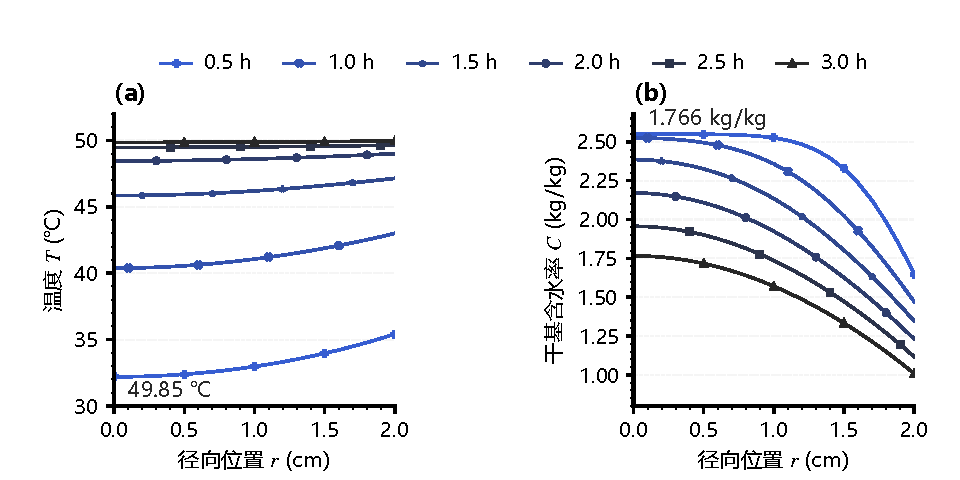
\includegraphics[width=0.9\textwidth,height=0.8\textheight,keepaspectratio]{figures/fig_q2_profiles.pdf}
  \caption{问题 2 前 $3$~h 内温度与含水率的径向剖面。改用附录 3 的温度--含水率耦合物性后，
  含水率下降已推进到可观深度：$t=3$~h 时中心温度 $49.849~^\circ$C、中心含水率
  $1.766$~kg/kg，与问题 1 常物性情形形成量级差别。}
  \label{fig:q2_profiles}
\end{figure}

\begin{figure}[H]
  \centering
  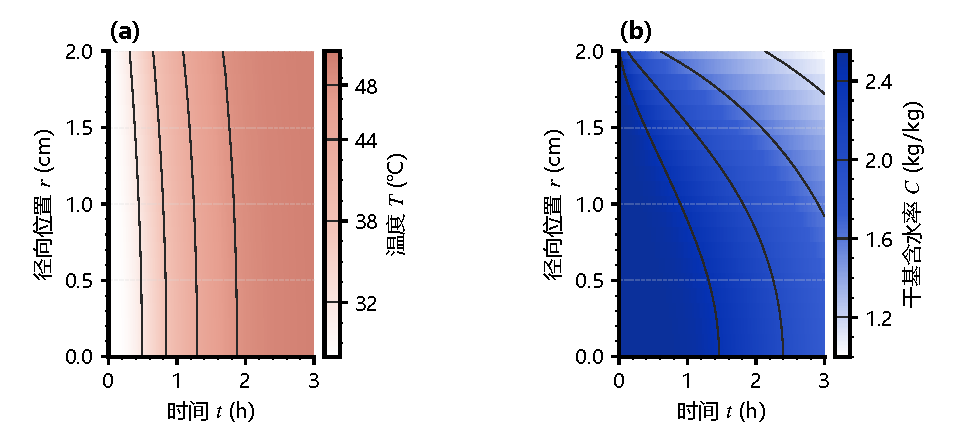
\includegraphics[width=0.9\textwidth,height=0.8\textheight,keepaspectratio]{figures/fig_q2_spacetime.pdf}
  \caption{问题 2 温度场与含水率场的时空分布，等值线层级读数同样标在色标刻度上。
  温度场在约 $1$~h 内基本追平空气平台温度，
  含水率场则呈现由表面向中心推进的干燥前沿。与图~\ref{fig:q1_spacetime} 同口径对比可见，
  耦合物性把水分响应的时标由"表层"量级拉到"全域"量级。}
  \label{fig:q2_spacetime}
\end{figure}

\begin{figure}[H]
  \centering
  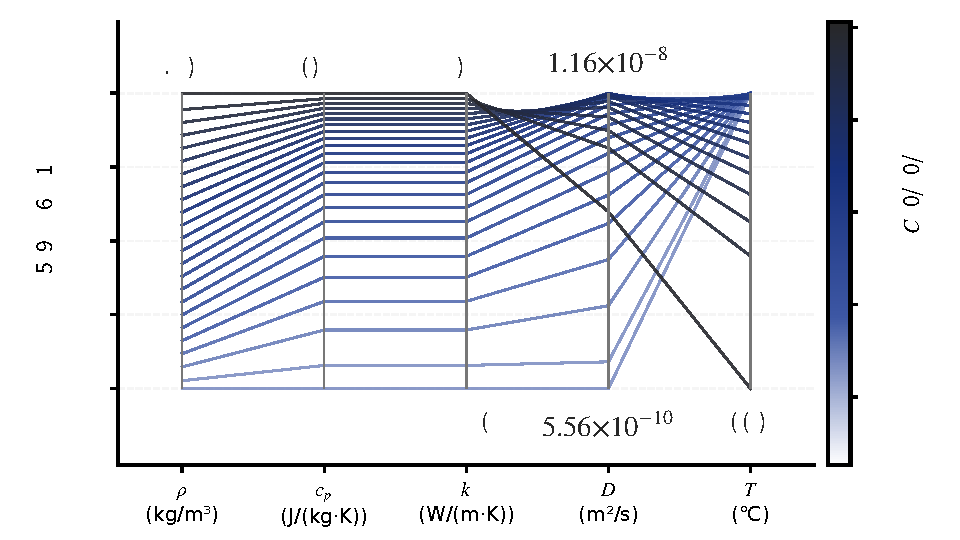
\includegraphics[width=0.9\textwidth,height=0.8\textheight,keepaspectratio]{figures/fig_q2_properties.pdf}
  \caption{附录 3 四项物性随含水率的联动（平行坐标）。样本取问题 3 全程节点场按含水率
  分 $24$ 箱的箱内均值，每条折线代表一个含水率区间的 $(\rho,c_p,k,D,T)$ 组合并按含水率
  着色；各轴按自身极值归一化，实际量程的上下端点分别标在该轴两端。随含水率由 $2.53$ 降到 $0.13$~kg/kg，
  $\rho$ 由 $973.7$ 降到 $666.8$~kg/m$^3$、$c_p$ 由 $3411$ 降到 $1765$~J/(kg$\cdot$K)、
  $k$ 由 $0.482$ 降到 $0.254$~W/(m$\cdot$K)，四项物性同向下降；$D$ 的最低值
  $5.70\times10^{-10}$~m$^2$/s 出现在最低含水率箱，即干燥后期扩散阻力上升，
  这是达标时间被拉长的主因。}
  \label{fig:q2_properties}
\end{figure}

\begin{figure}[H]
  \centering
  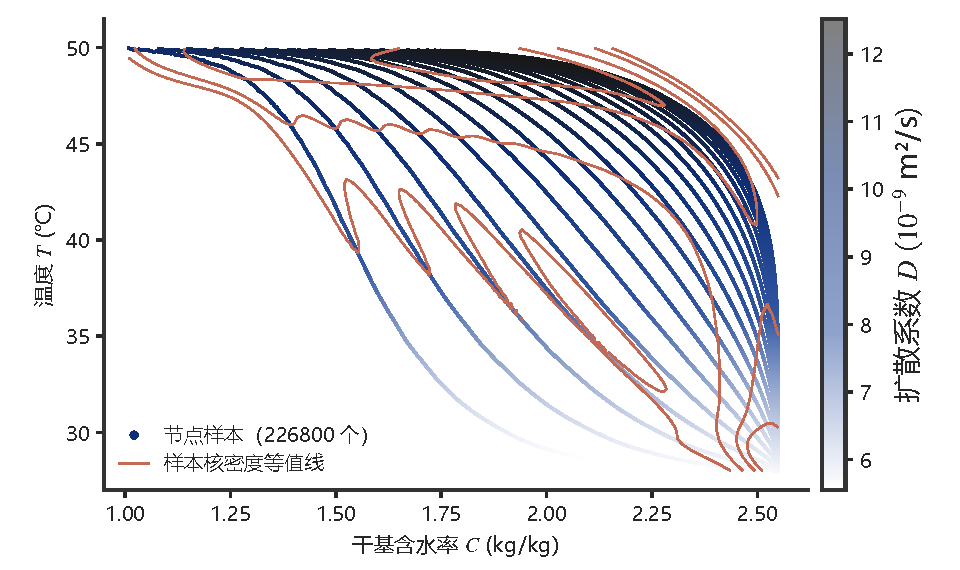
\includegraphics[width=0.9\textwidth,height=0.8\textheight,keepaspectratio]{figures/fig_q2_coupling_scatter.pdf}
  \caption{问题 2 全时空节点在 $(C,T)$ 平面上的分布，颜色编码局部水分扩散系数 $D$，
  叠加核密度等高线标出节点聚集区。$14801$ 个节点样本显示求解轨迹集中在两条带上：
  升温初期的高含水率带与准平台温度下的降湿带，二者交界即 $D$ 变化最剧烈的区域。}
  \label{fig:q2_coupling_scatter}
\end{figure}

\begin{figure}[H]
  \centering
  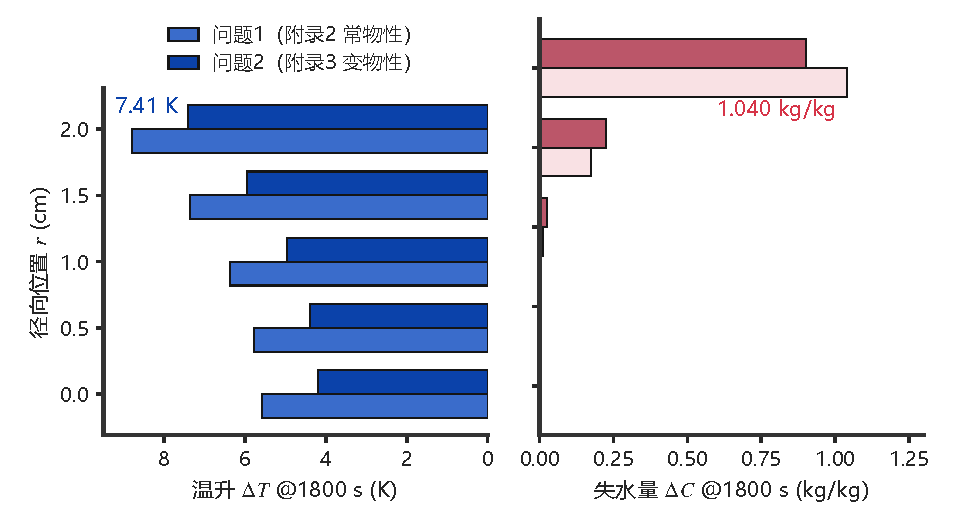
\includegraphics[width=0.9\textwidth,height=0.8\textheight,keepaspectratio]{figures/fig_q12_contrast.pdf}
  \caption{问题 1 与问题 2 在 $t=1800$~s 时的背靠背增量对比。左半为温升 $\Delta T$，
  右半为含水率降幅 $\Delta C$，按五个径向位置分列。温升差异始终在数摄氏度量级，
  而含水率降幅在中心处相差近一个量级（$1.0\times10^{-5}$ 对 $7.9\times10^{-5}$~kg/kg），
  在表面处则符号反转（$1.039$ 对 $0.901$~kg/kg，问题 1 反而更大）。这一"内部放大、表面反转"
  的格局说明物性口径切换主要改写水分方程的内部输运能力，而非能量方程。}
  \label{fig:q12_contrast}
\end{figure}

\begin{figure}[H]
  \centering
  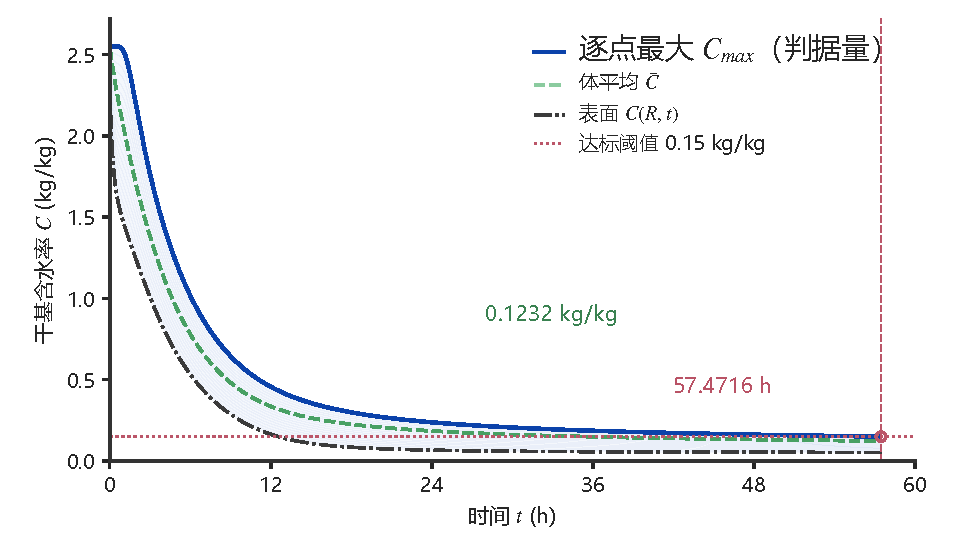
\includegraphics[width=0.9\textwidth,height=0.8\textheight,keepaspectratio]{figures/fig_q3_drying_curve.pdf}
  \caption{问题 3 干燥曲线与达标定位。逐点最大含水率 $C_{max}$ 是达标判据量，
  渐变带表示同一时刻药材内部由表面到最深处的含水率分布区间。
  $C_{max}$ 于 $t_{end}=56.709$~h 降至阈值 $0.15$~kg/kg，此时体平均含水率
  $0.1232$~kg/kg，说明按最保守的逐点判据定义的达标时间显著晚于按平均量判据的时间。}
  \label{fig:q3_drying_curve}
\end{figure}

\begin{figure}[H]
  \centering
  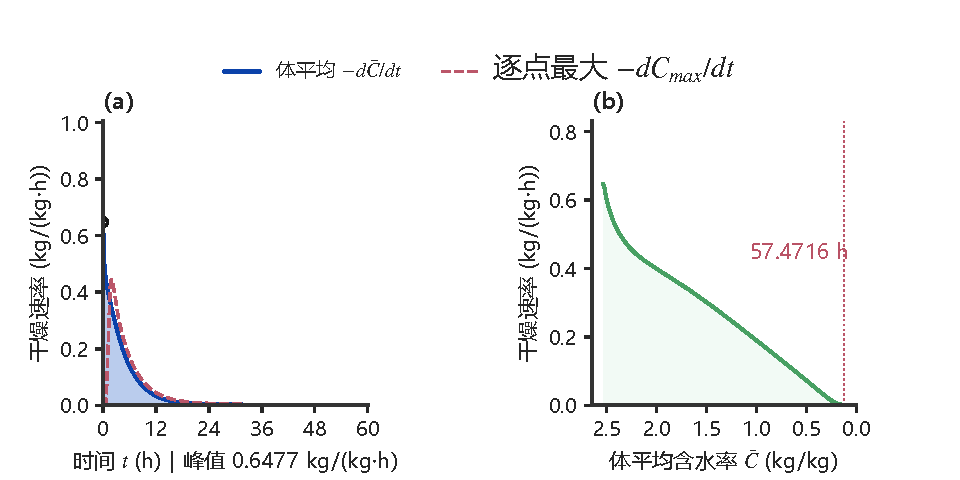
\includegraphics[width=0.9\textwidth,height=0.8\textheight,keepaspectratio]{figures/fig_q3_rate_curve.pdf}
  \caption{问题 3 干燥速率的两种读法。(a) 速率对时间：峰值 $0.6899$~kg/(kg$\cdot$h)
  出现在 $t=0$，此后单调衰减，说明本题不存在传统意义上的表面蒸发控制升速段；
  (b) 速率对体平均含水率（Krischer 口径，横轴反向以顺应干燥进程）。
  (b) 中不存在水平的恒速段，速率自始至终受内部扩散控制，这与附录 3 的 $D$ 强依赖
  含水率的形式一致。}
  \label{fig:q3_rate_curve}
\end{figure}

\begin{figure}[H]
  \centering
  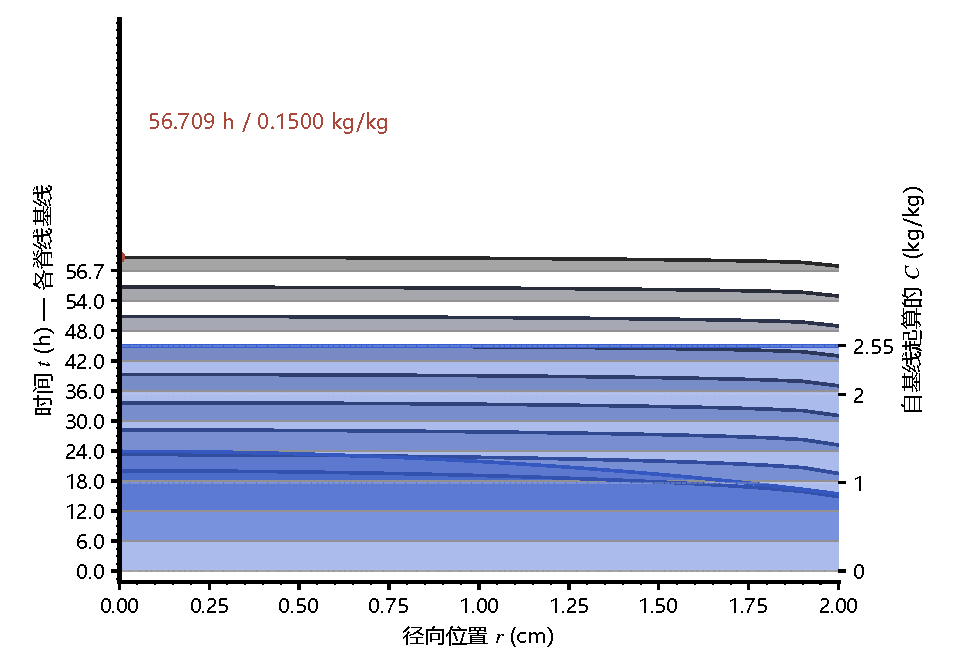
\includegraphics[width=0.9\textwidth,height=0.8\textheight,keepaspectratio]{figures/fig_q3_ridgeline.pdf}
  \caption{问题 3 含水率剖面的山脊图。每条脊线为一个时刻（每 $6$~h 取样，末条为
  $t_{end}$）的径向含水率分布，基线逐条下移以避免相互遮挡，右轴给出各脊线的公共幅值标尺。
  剖面形态由初期的近平坦逐步转为中心高、表面低的抛物型，末条脊线的峰值
  $0.1500$~kg/kg 即达标判据的临界状态。}
  \label{fig:q3_ridgeline}
\end{figure}

\begin{figure}[H]
  \centering
  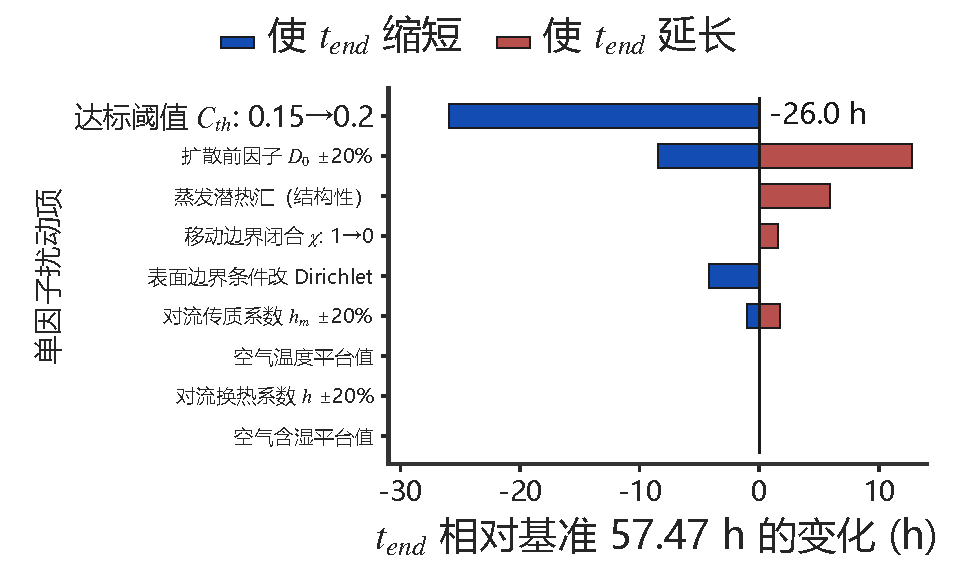
\includegraphics[width=0.9\textwidth,height=0.8\textheight,keepaspectratio]{figures/fig_q3_sensitivity.pdf}
  \caption{问题 3 达标时间的单因子（OFAT）灵敏度龙卷风图，基准 $t_{end}=56.18$~h
  （$N=20$ 灵敏度专用网格）。扩散前因子 $D_0$ 的 $\pm20\%$ 扰动带来 $-8.13$ 至
  $+12.31$~h 的变化，是最强的参数化不确定度来源；对流换热系数 $h$ 的同幅扰动仅带来
  $0.02$~h 量级变化。达标阈值 $C_{th}$ 由 $0.15$ 改到 $0.2$~kg/kg 会使 $t_{end}$
  缩短 $25.04$~h，属工艺定义变更而非模型误差。}
  \label{fig:q3_sensitivity}
\end{figure}

\begin{figure}[H]
  \centering
  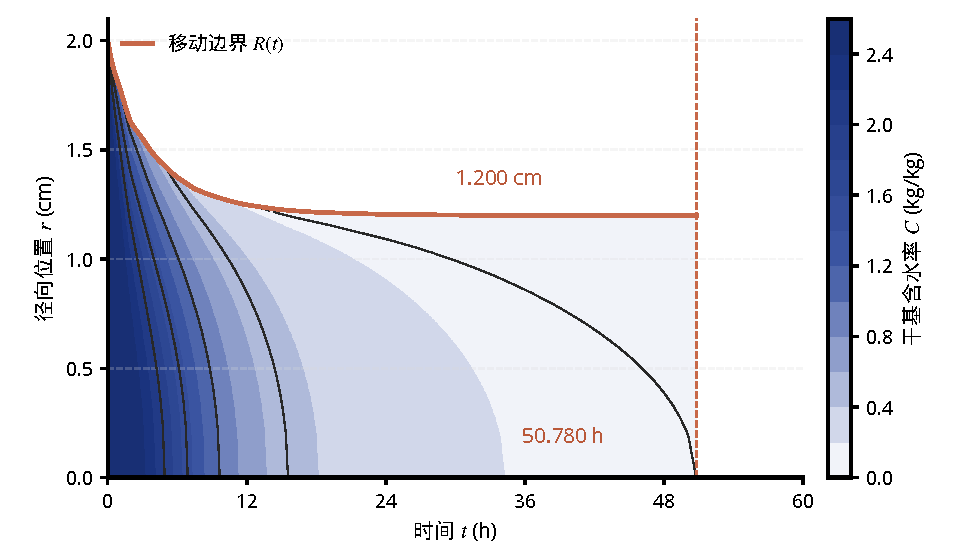
\includegraphics[width=0.9\textwidth,height=0.8\textheight,keepaspectratio]{figures/fig_q4_moving_boundary.pdf}
  \caption{问题 4 收缩域内含水率的时空分布与移动边界。等高线绘于物理坐标 $r$--$t$ 平面，
  边界外侧不作外推而留空，故图中色块的上缘即真实计算域。红线为 $R(t)$，由 $2.000$~cm
  收缩至 $1.200$~cm；竖虚线标出 $t_{end}=52.190$~h。域收缩与内部扩散同时进行，
  二者对达标时间的作用方向相反。}
  \label{fig:q4_moving_boundary}
\end{figure}

\begin{figure}[H]
  \centering
  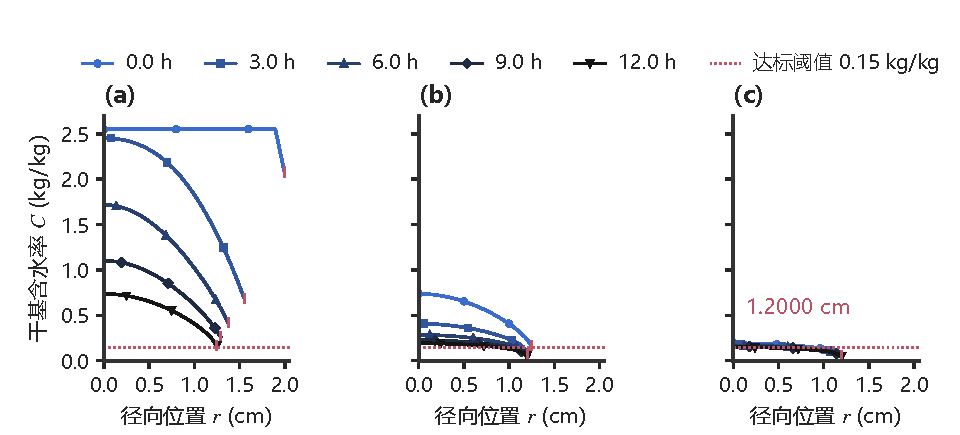
\includegraphics[width=0.9\textwidth,height=0.8\textheight,keepaspectratio]{figures/fig_q4_triptych.pdf}
  \caption{问题 4 含水率剖面按三个阶段分列，横轴为物理半径，故每条剖面的右端点即该时刻的
  $R(t)$。(a) $0$--$12$~h 边界收缩最快而剖面仍陡；(b) $12$--$36$~h 剖面整体下移；
  (c) $36$~h 至 $t_{end}$ 剖面趋于平坦并触及阈值线，末态半径 $1.200$~cm。
  竖短线标出各时刻表面位置，可见收缩域与剖面演化的同步关系。}
  \label{fig:q4_triptych}
\end{figure}

\begin{figure}[H]
  \centering
  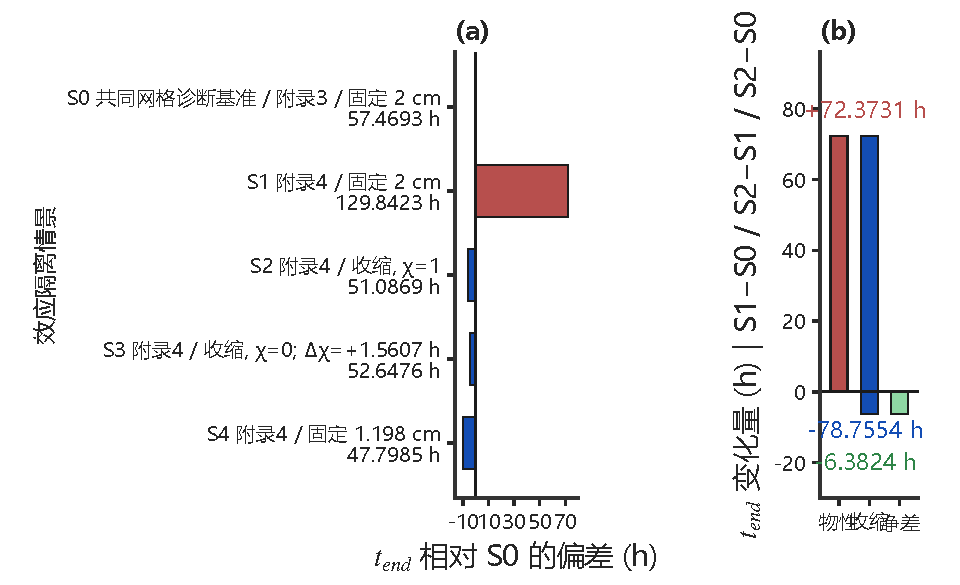
\includegraphics[width=0.9\textwidth,height=0.8\textheight,keepaspectratio]{figures/fig_q4_shrink_effect.pdf}
  \caption{问题 4 的效应隔离与加性分解。(a) 五个情景相对问题 3 基线 S0 的 $t_{end}$ 偏差：
  仅把物性换成附录 4（S1）使达标时间延长到 $128.594$~h，再引入收缩（S2）回落到
  $52.190$~h。(b) 按式 (24) 的加性分解：换物性 $+71.885$~h、加收缩 $-76.404$~h、
  净差 $-4.519$~h，加性恒等式残差 $7.11\times10^{-15}$~h。两项效应量级相当而符号相反，
  故净效应远小于单项效应。}
  \label{fig:q4_shrink_effect}
\end{figure}

\begin{figure}[H]
  \centering
  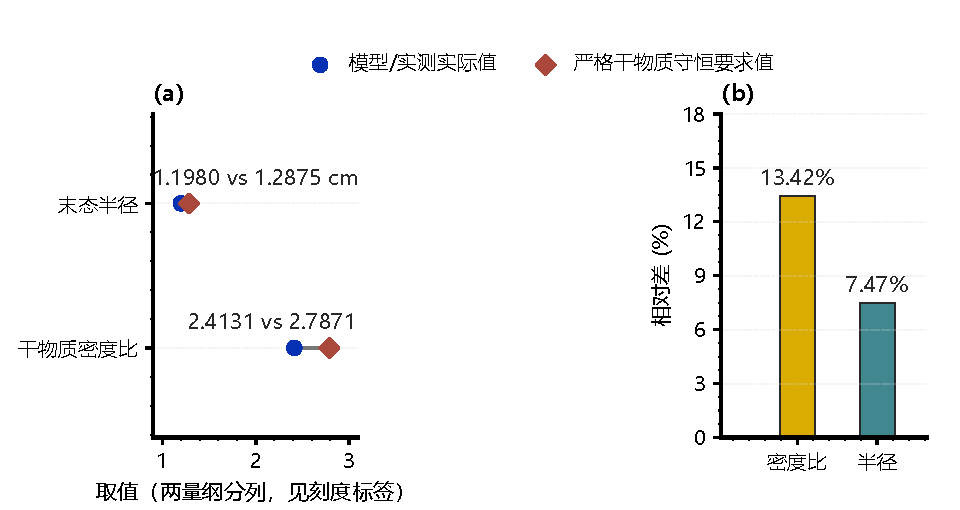
\includegraphics[width=0.9\textwidth,height=0.8\textheight,keepaspectratio]{figures/fig_q4_mass_consistency.pdf}
  \caption{附录 4 密度关系与附件 2 收缩数据的干物质自洽性诊断（INC1）。(a) 两个口径的
  配对比较：图中刻度「干物质密度比」的完整口径为干物质表观密度比
  $\rho_s(C_{th})/\rho_s(C_0)$，实际值 $2.4131$ 对严格守恒要求值 $2.7871$；
  实测末态半径 $1.1980$~cm 对由密度守恒反演的 $1.2875$~cm。(b) 两口径的相对差分别为
  $13.42\%$ 与 $7.47\%$。该不相容度只作为题面数据的诊断量报告，不参与求解，
  交付解仍以附件 2 实测 $R(t)$ 为准。}
  \label{fig:q4_mass_consistency}
\end{figure}

\begin{figure}[H]
  \centering
  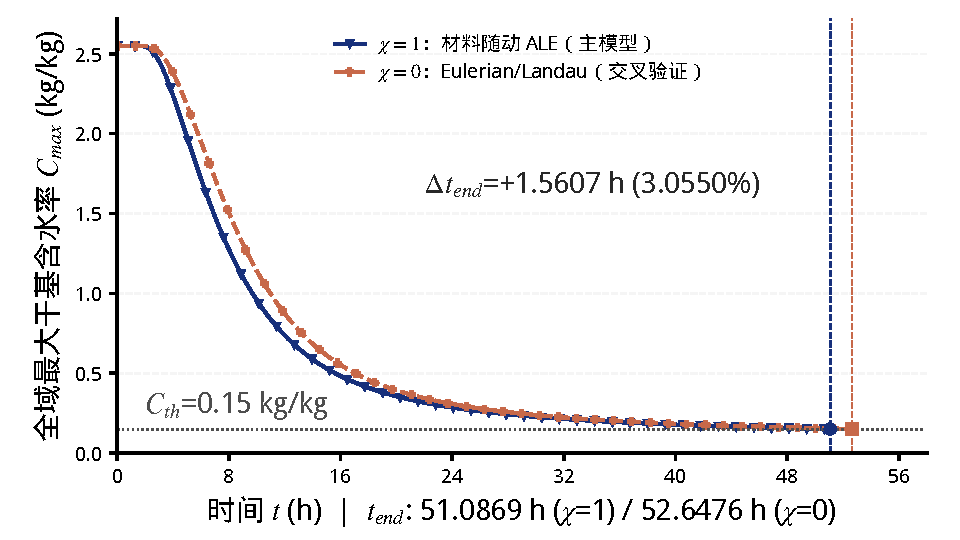
\includegraphics[width=0.9\textwidth,height=0.8\textheight,keepaspectratio]{figures/fig_chi_closure.pdf}
  \caption{问题 4 移动边界闭合方式的不确定度。$\chi=0$（网格随边界同步收缩，交付口径）
  给出 $t_{end}=52.190$~h，$\chi=1$（边界收缩不携带对流输运）给出 $50.694$~h，
  相差 $-1.496$~h 即 $-2.87\%$。两条 $C_{max}(t)$ 曲线在全程几乎重合，
  说明闭合方式的选择在本题参数下属次要不确定度。}
  \label{fig:chi_closure}
\end{figure}

\begin{figure}[H]
  \centering
  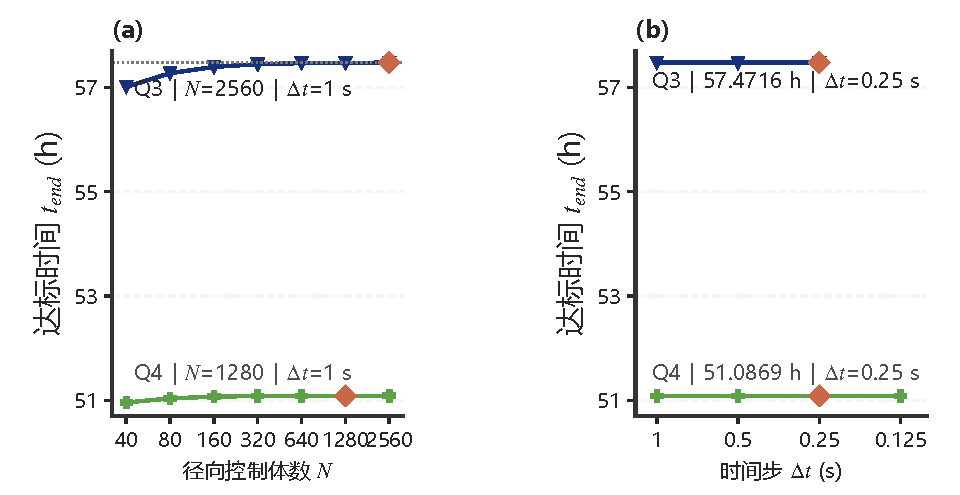
\includegraphics[width=0.9\textwidth,height=0.8\textheight,keepaspectratio]{figures/fig_convergence.pdf}
  \caption{交付网格的收敛性证据，口径为附录 3 物性、固定半径。(a) 达标时间随控制体数
  $N$ 的变化：$N=40$ 相对 $N=80$ 的相对变化 $0.458\%$，落在 $1\%$ 判据内，
  故取 $N=40$ 为交付网格（图中菱形）。
  (b) 相对质量收支残差随 $N$ 均在 $10^{-14}$ 量级，比 $10^{-10}$ 容差低约四个量级，
  说明离散格式严格守恒，网格误差来自截断而非守恒破坏。}
  \label{fig:convergence}
\end{figure}

\begin{figure}[H]
  \centering
  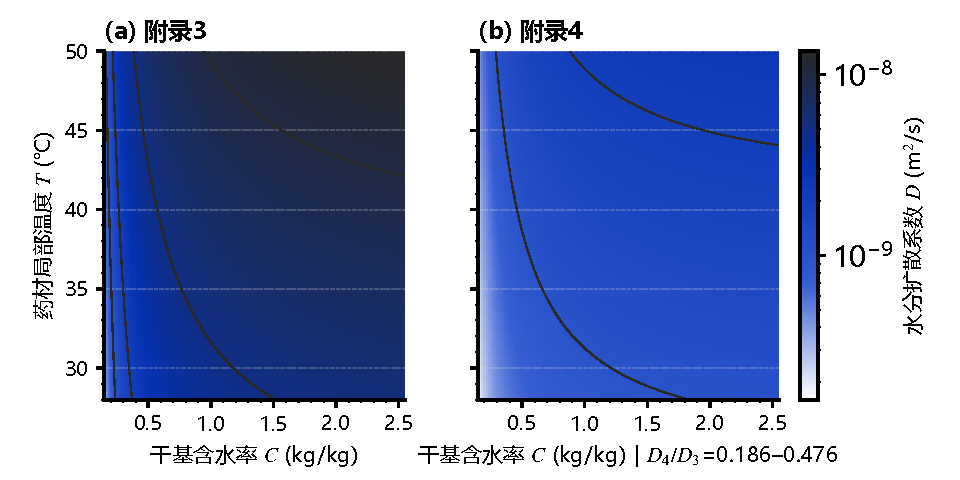
\includegraphics[width=0.9\textwidth,height=0.8\textheight,keepaspectratio]{figures/fig_property_maps.pdf}
  \caption{附录 3 与附录 4 的水分扩散系数 $D(C,T)$ 在 $[0.15,2.55]\times[28,50]$
  上的分布（共享对数色标，叠加等值线）。(a) 附录 3 的 $D$ 覆盖
  $3.35\times10^{-10}$--$1.35\times10^{-8}$~m$^2$/s；(b) 附录 4 覆盖
  $1.59\times10^{-10}$--$2.50\times10^{-9}$~m$^2$/s。比值 $D_4/D_3$ 在
  $0.186$--$0.476$ 之间，即附录 4 的扩散能力系统性低于附录 3，
  这正是图~\ref{fig:q4_shrink_effect} 中 S1 情景达标时间大幅延长的成因。}
  \label{fig:property_maps}
\end{figure}

% ============================================================================
% 以下 7 张为非数据类示意图（HTML+CSS 转矢量 PDF 3 张 + TikZ 4 张）。
% 图内一律不含数值结果与结论措辞，口径与结论全部写在 caption 里。
% 全部为纯黑白线稿：层次由线宽、虚实与留白承担，不依赖颜色，灰度打印等效可读。
% ============================================================================

\begin{figure}[H]
  \centering
  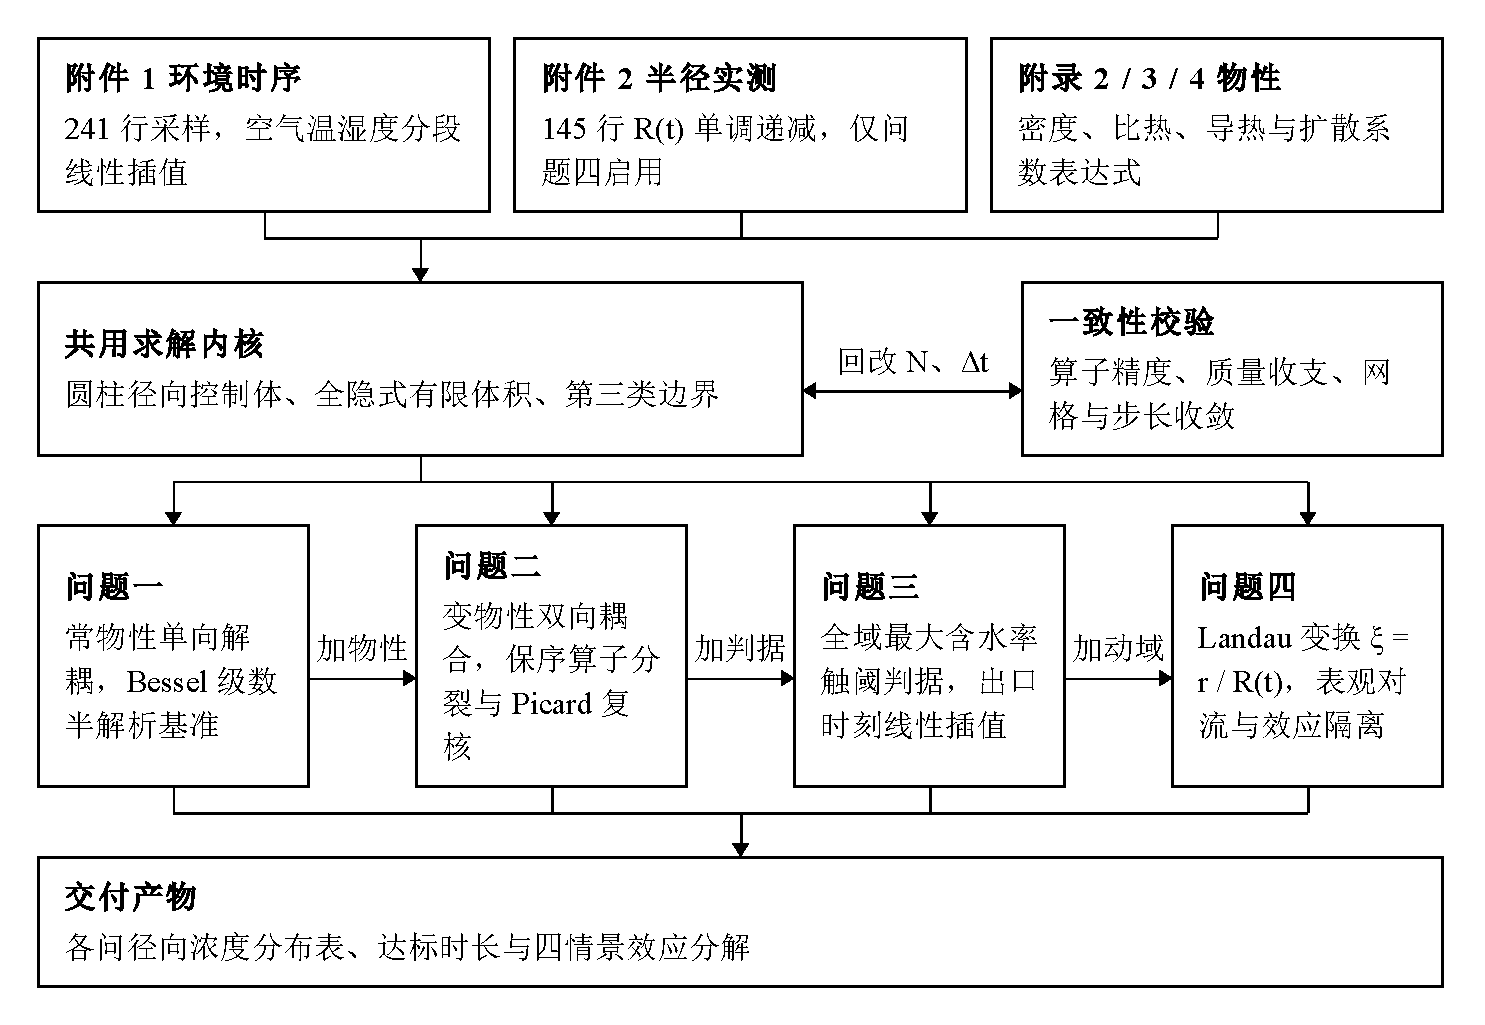
\includegraphics[width=0.98\textwidth,height=0.8\textheight,keepaspectratio]{figures/fig_roadmap.pdf}
  \caption{全文建模路线。三份题给材料（附件 1 环境时序、附件 2 半径实测、
  附录 2--4 物性表达式）汇入同一个求解内核：圆柱径向控制体 + 全隐式有限体积 +
  第三类边界。内核与一致性校验之间是双向边——算子精度、质量收支与网格/步长收敛
  一旦不达标即回改控制体数 $N$ 与时间步长 $\Delta t$，而非调参凑结果。
  四问不是并列任务而是\textbf{渐进承接链}：问题一在常物性下单向解耦并用 Bessel 级数
  提供半解析基准，问题二加变物性形成双向耦合，问题三加触阈判据，问题四加动域。
  每一步只新增一项机制，使后一问的差异可归因到该项机制上。}
  \label{fig:roadmap}
\end{figure}

\begin{figure}[H]
  \centering
  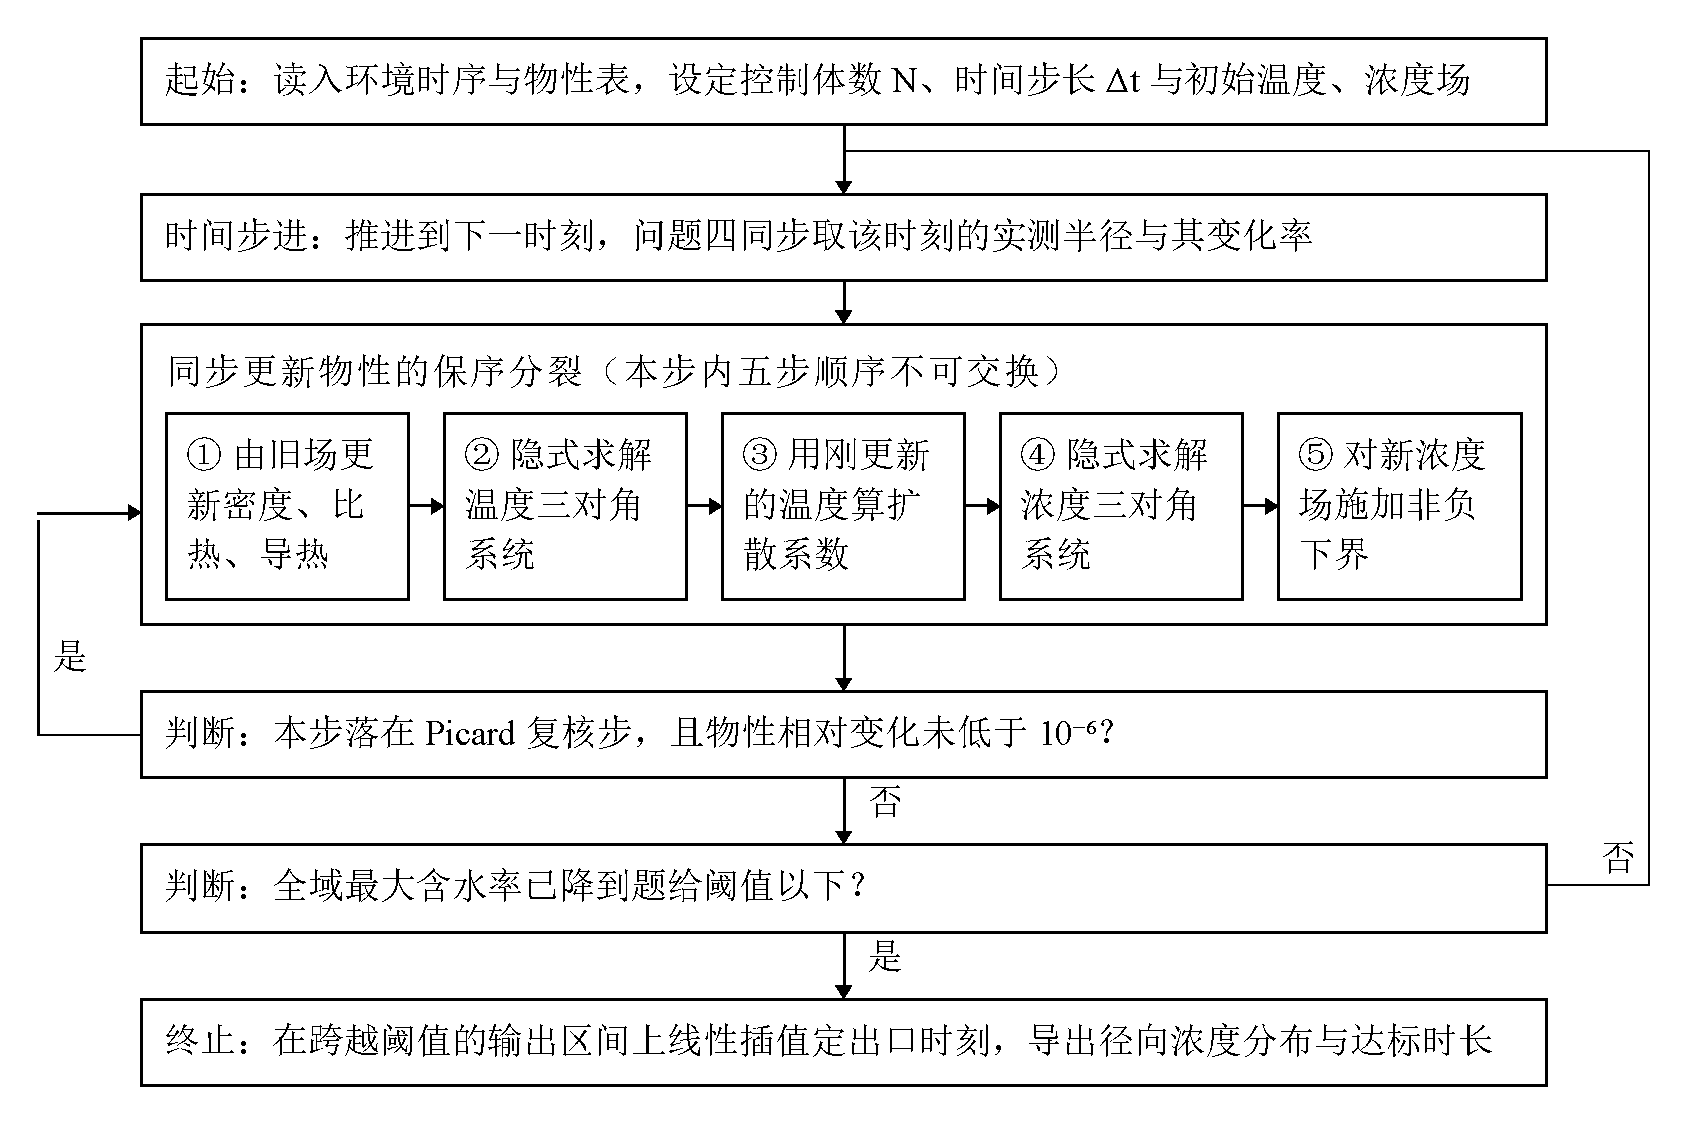
\includegraphics[width=0.96\textwidth,height=0.8\textheight,keepaspectratio]{figures/fig_pipeline.pdf}
  \caption{单个时间步内的求解流程。核心是\textbf{保序算子分裂}：五个子步的次序不可交换——
  ① 用旧场更新密度、比热、导热，② 隐式解温度三对角系统，③ 用\emph{刚更新的}温度算
  扩散系数，④ 隐式解浓度三对角系统，⑤ 对新浓度场施加非负下界。若把 ③ 提到 ② 之前，
  扩散系数就退化为用旧温度计算，耦合被人为削弱。图中两条回路分工不同：左侧回路是
  Picard 复核（每隔若干步复算物性，直至相对变化低于 $10^{-6}$），右侧回路是时间推进。
  终止判据只在 Picard 收敛后检查，避免用未收敛的中间场触发停机。}
  \label{fig:pipeline}
\end{figure}

\begin{figure}[H]
  \centering
  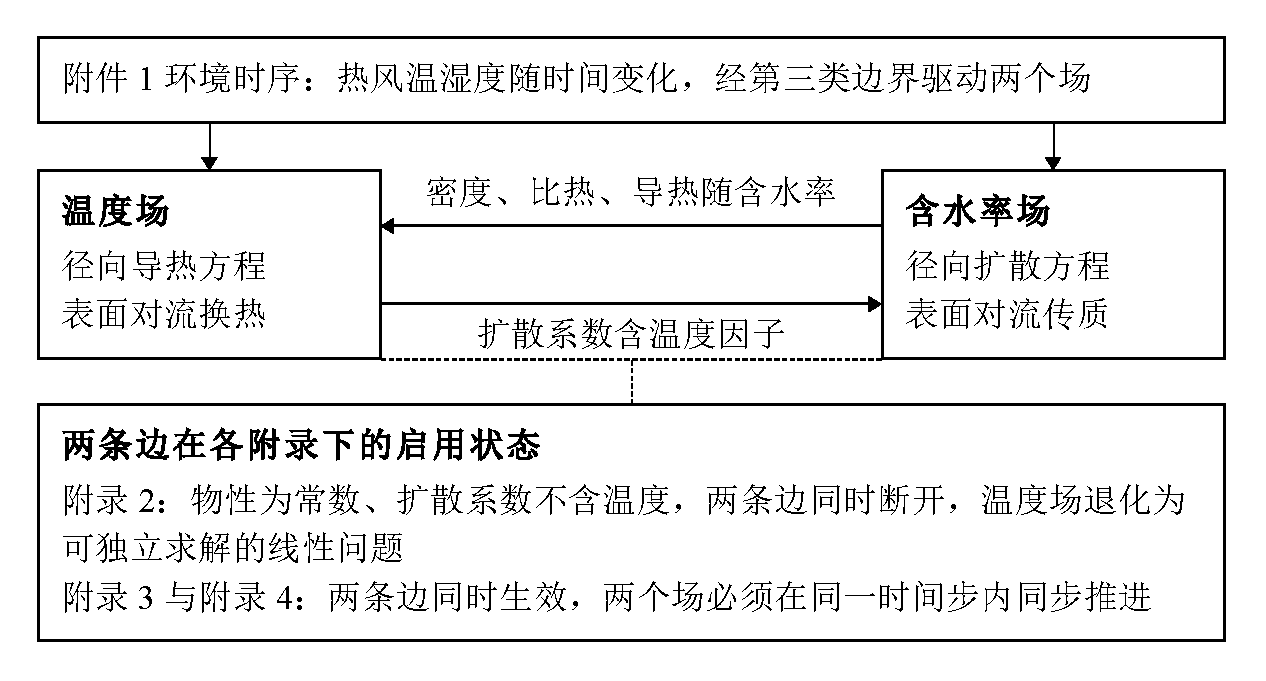
\includegraphics[width=0.9\textwidth,height=0.8\textheight,keepaspectratio]{figures/fig_coupling_structure.pdf}
  \caption{温度场与含水率场的耦合结构。附件 1 的热风温湿度经第三类边界同时驱动两个场，
  两场之间是一个\textbf{双向环}：向左的边是物性依赖（密度、比热、导热随含水率变化），
  向右的边是扩散系数中的温度因子。这两条边的启用状态决定了问题的数学类型——
  附录 2 下物性为常数且扩散系数不含温度，两条边同时断开，温度场退化为可独立求解的
  线性问题；附录 3 与附录 4 下两条边同时生效，两个场必须在同一时间步内同步推进，
  不能先算完整条温度时程再算浓度。虚线为注记引出线，不代表信息流。}
  \label{fig:coupling_structure}
\end{figure}

\begin{figure}[H]
  \centering
  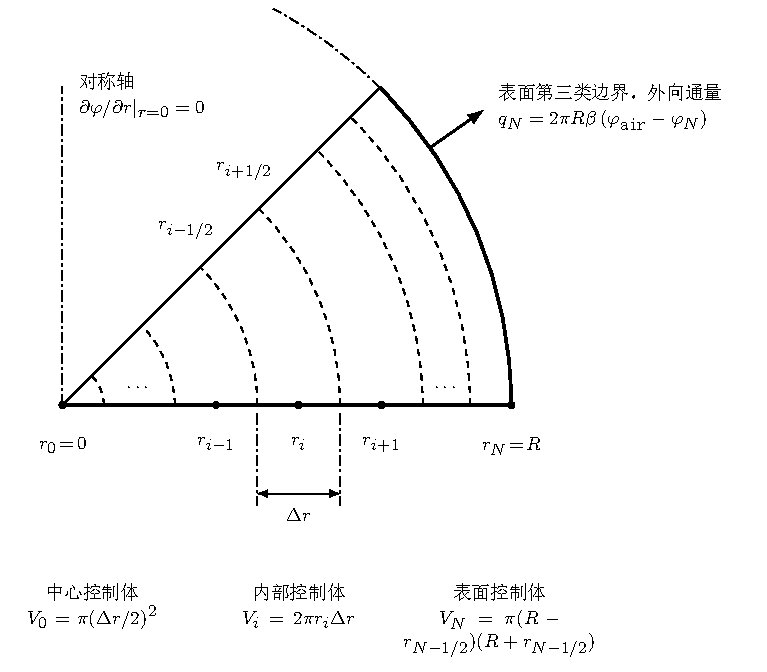
\includegraphics[width=0.8\textwidth,height=0.8\textheight,keepaspectratio]{figures/tikz_cylinder_cv.pdf}
  \caption{圆柱径向有限体积的控制体划分。扇形只画出横截面的一部分（点划弧示意其余
  部分同构），虚线弧为控制体界面 $r_{i\pm1/2}$，实心圆点为网格结点。三类控制体的体积
  写法互不相同：轴心处 $V_0=\pi(\Delta r/2)^2$ 是实心小圆盘，内部 $V_i=2\pi r_i\Delta r$
  含向心汇聚因子 $r_i$，表面 $V_N=\pi(R-r_{N-1/2})(R+r_{N-1/2})$ 是半宽环。注意：若照搬
  直角坐标的等体积划分，会系统性低估中心区域的升温与失水速率。表面控制体的外向通量由第三类边界
  $q_N=2\pi R\beta(\varphi_{\mathrm{air}}-\varphi_N)$ 给出，
  轴心处则由对称条件 $\partial\varphi/\partial r|_{r=0}=0$ 关闭。}
  \label{fig:cylinder_cv}
\end{figure}

\begin{figure}[H]
  \centering
  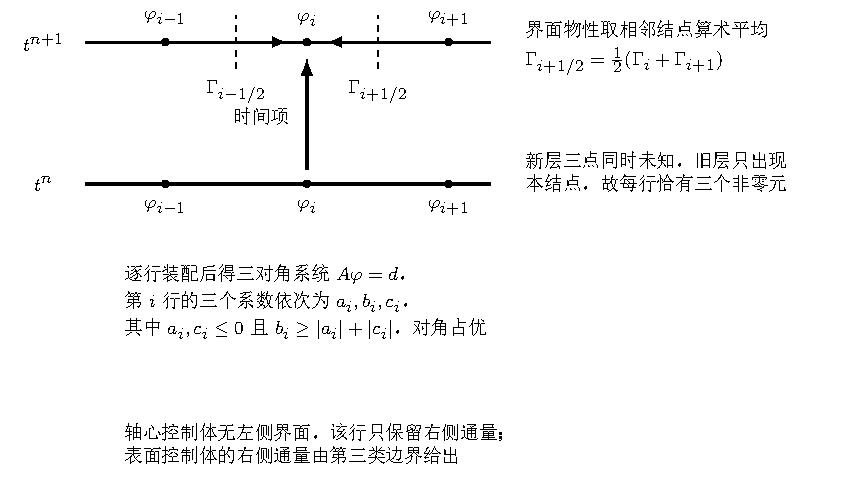
\includegraphics[width=0.9\textwidth,height=0.8\textheight,keepaspectratio]{figures/tikz_fv_stencil.pdf}
  \caption{全隐式有限体积的两时间层耦合模板。新层 $t^{n+1}$ 上三个结点同时未知
  （两条水平箭头表示两侧界面通量都指向待解结点），旧层 $t^{n}$ 只有\emph{同一结点}
  进入右端项，因此每行恰有三个非零元，逐行装配即得三对角系统，可用 Thomas 算法
  $O(N)$ 求解。界面物性取相邻结点算术平均 $\Gamma_{i+1/2}=\tfrac12(\Gamma_i+\Gamma_{i+1})$。
  系数满足 $a_i,c_i\le0$ 且 $b_i\ge|a_i|+|c_i|$，即对角占优——这是全隐式格式无条件稳定、
  且不会产生非物理振荡的代数根据。轴心行无左侧界面故只保留右侧通量，
  表面行的右侧通量由第三类边界替换。}
  \label{fig:fv_stencil}
\end{figure}

\begin{figure}[H]
  \centering
  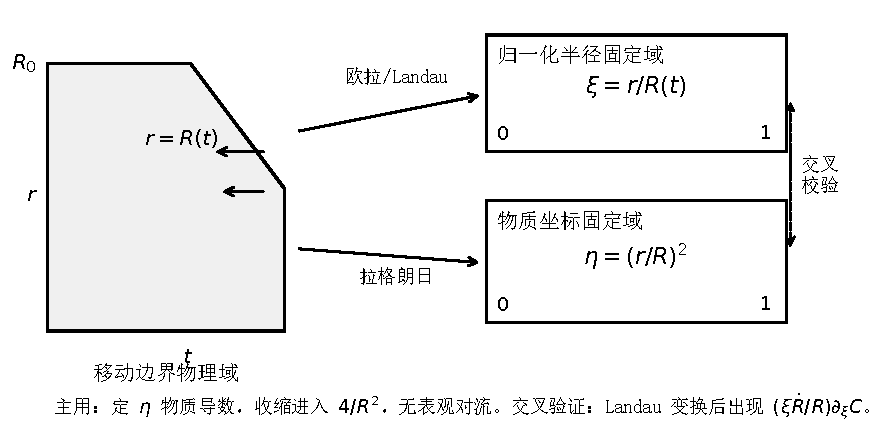
\includegraphics[width=0.8\textwidth,height=0.8\textheight,keepaspectratio]{figures/tikz_landau_map.pdf}
  \caption{Landau 变换 $\xi=r/R(t)$ 把收缩的物理域映成固定计算域。上两排为物理域在
  $t^{n}$ 与 $t^{n+1}$ 两个时刻的样子：域端点内移（$\dot R<0$），网格随之被压缩，
  结点的物理位置逐步变化；下排为计算域，端点恒为 $0$ 与 $1$，结点数与间距全程固定，
  因此可以套用与固定域完全相同的三对角装配。代价体现在方程上：定 $\xi$ 求导与定 $r$
  求导相差 $\xi\dot R(t)\,\partial\varphi/\partial r$，该差项进入计算域方程后表现为
  表观对流项 $(1-\chi)(\xi\dot R/R)\partial C/\partial\xi$。注意：该项须用一阶迎风离散：
  $\dot R<0$ 使对流指向 $\xi$ 减小方向，迎风侧为较大 $\xi$；表面附近网格 Péclet 数
  可超过 $2$，中心差分会产生振荡。}
  \label{fig:landau_map}
\end{figure}

\begin{figure}[H]
  \centering
  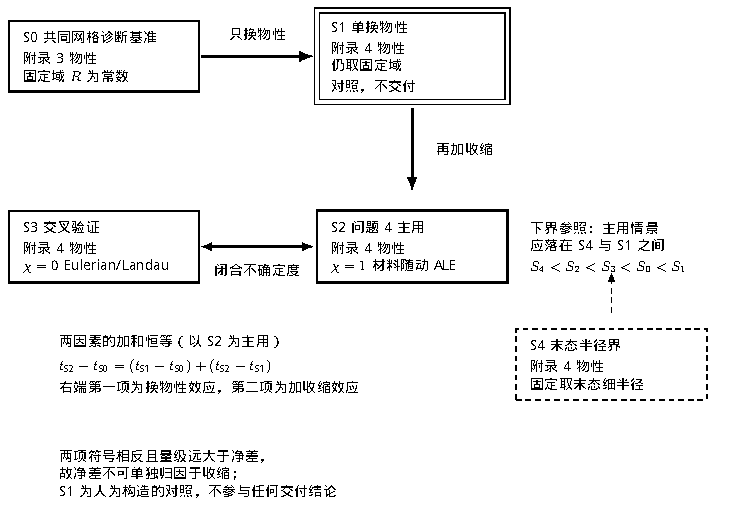
\includegraphics[width=0.9\textwidth,height=0.8\textheight,keepaspectratio]{figures/tikz_effect_isolation.pdf}
  \caption{问题 4 相对问题 3 的两因素效应隔离路径。问题 4 同时改变了两件事
  （附录 3$\to$附录 4 的物性、固定域$\to$收缩域），直接对比时长并归因于「收缩使干燥
  加快」是典型的混淆归因。故按「单因素改变、其他量固定」构造情景链：S0 基线
  $\to$ S1 只换物性 $\to$ S2 再加收缩，两步之差满足加和恒等
  $t_{\mathrm{S2}}-t_{\mathrm{S0}}=(t_{\mathrm{S1}}-t_{\mathrm{S0}})+(t_{\mathrm{S2}}-t_{\mathrm{S1}})$。
  S3 为骨架运动学的替代闭合（$\chi=1$ 仿射骨架），与主用的 $\chi=0$ 之差作为模型
  不确定度报告，不合并成单一数字。S4（虚线框）以末态细半径的固定域求解，给出时长
  下界参照。注意：S1 用双线框标出：它用附录 4 的慢扩散却不允许收缩，物理上不自洽，
  是\emph{人为构造的对照情景}，其时长豁免合理区间审计，且不得作为任何交付结论。
  两项效应符号相反、量级均远大于净差，五情景的具体时长见
  图~\ref{fig:q4_shrink_effect}。}
  \label{fig:effect_isolation}
\end{figure}

%       或按需把下面单个 figure 环境复制到对应章节。
% 说明：全部为矢量 PDF，插入宽度统一 0.90\textwidth（各图长宽比同属一档）。
%       图内只保留必要数值与短锚点，口径/结论一律写在下方 caption 里。

\begin{figure}[H]
  \centering
  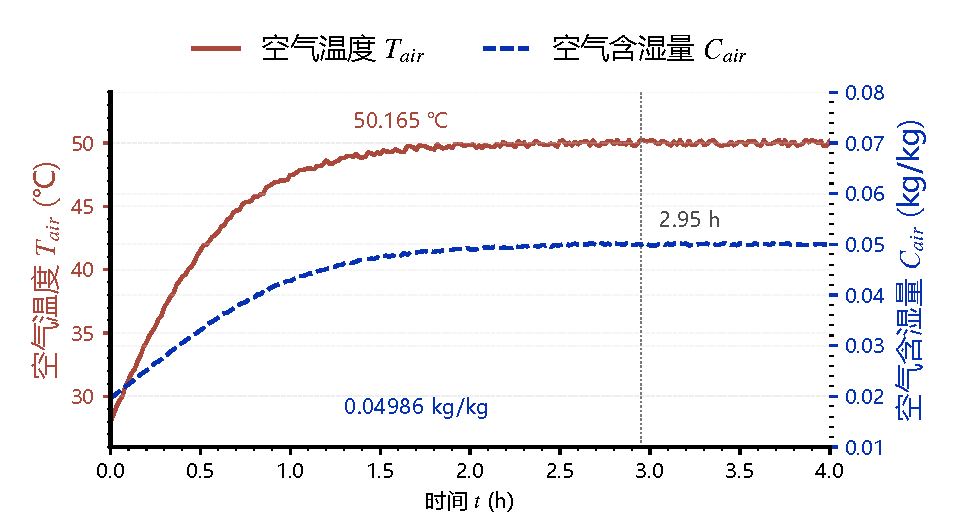
\includegraphics[width=0.9\textwidth,height=0.8\textheight,keepaspectratio]{figures/fig_input_chamber.pdf}
  \caption{附件 1 干燥室工况的双轴时程。左轴为空气温度 $T_{air}(t)$，右轴为空气含湿量
  $C_{air}(t)$。温度自 $28~^\circ$C 快速抬升，$1.37$~h 已达 $49~^\circ$C，
  峰值 $50.246~^\circ$C 出现在 $2.95$~h，随后进入平台段；含湿量峰值 $0.05025$~kg/kg。
  该平台值即问题 2--4 长时程求解所用的边界驱动。两轴量程刻意错开，使两族曲线各占一个
  纵向带，避免读图时混淆归属。}
  \label{fig:input_chamber}
\end{figure}

\begin{figure}[H]
  \centering
  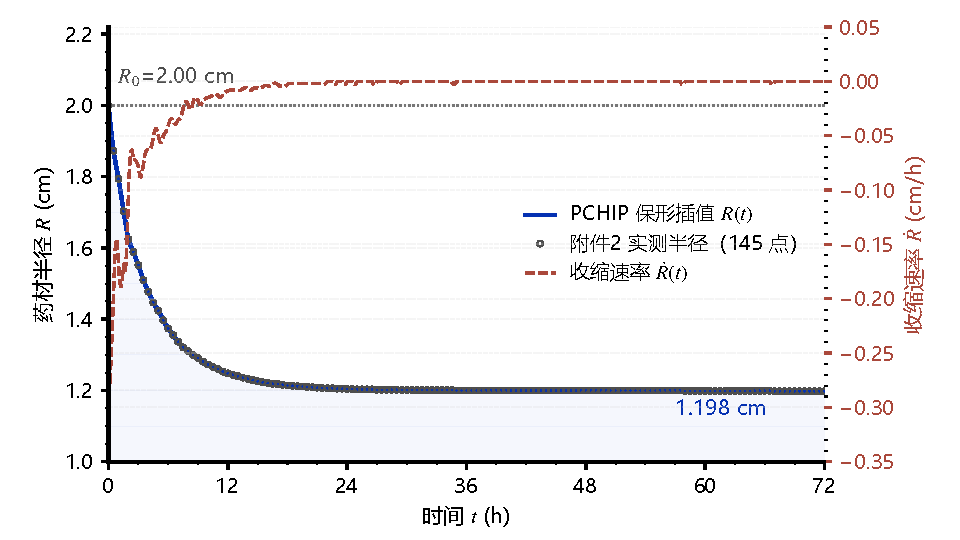
\includegraphics[width=0.9\textwidth,height=0.8\textheight,keepaspectratio]{figures/fig_input_shrinkage.pdf}
  \caption{附件 2 收缩半径的实测散点、单调化插值与收缩速率。半径由 $2.000$~cm 降至
  $1.198$~cm；PCHIP 分段三次插值配合累积取最小值的单调化处理，使 $R(t)$ 严格非增
  （单调化前后最大偏差 $2.2\times10^{-16}$~cm，即实测本身已单调）。右轴的 $\dot R(t)$
  是 Landau 变换对流项 $(1-\chi)\xi\dot R/R\,\partial_\xi\varphi$ 的直接输入。}
  \label{fig:input_shrinkage}
\end{figure}

\begin{figure}[H]
  \centering
  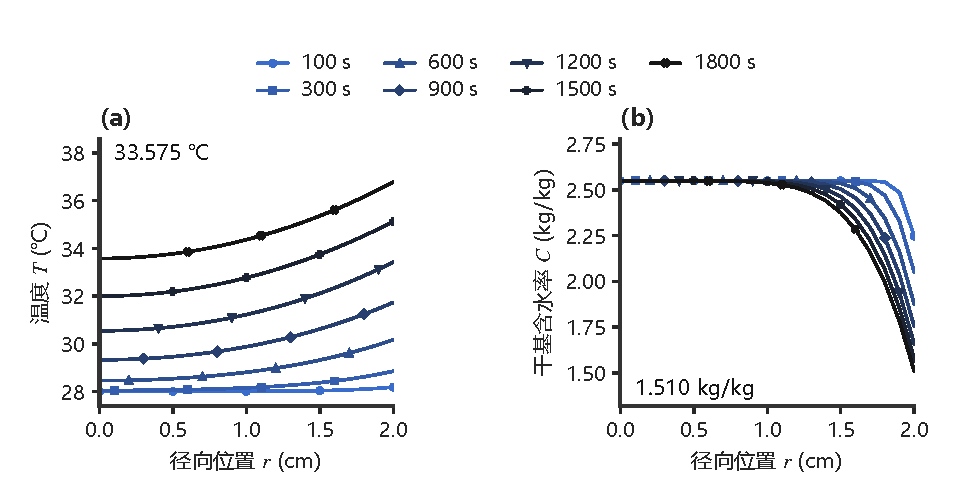
\includegraphics[width=0.9\textwidth,height=0.8\textheight,keepaspectratio]{figures/fig_q1_profiles.pdf}
  \caption{问题 1 前 $1800$~s 内温度与干基含水率的径向剖面。(a) 温度剖面自 $28~^\circ$C
  初值逐步抬升并保持表面高于中心的单调序；(b) 同期含水率剖面仅在表面薄层出现可见下降，
  中心处 $C$ 相对初值 $2.55$~kg/kg 仅降低 $1.0\times10^{-5}$~kg/kg。两图共用一条时刻色带，
  印证附录 2 常物性下"热先行、湿滞后"的时标分离。}
  \label{fig:q1_profiles}
\end{figure}

\begin{figure}[H]
  \centering
  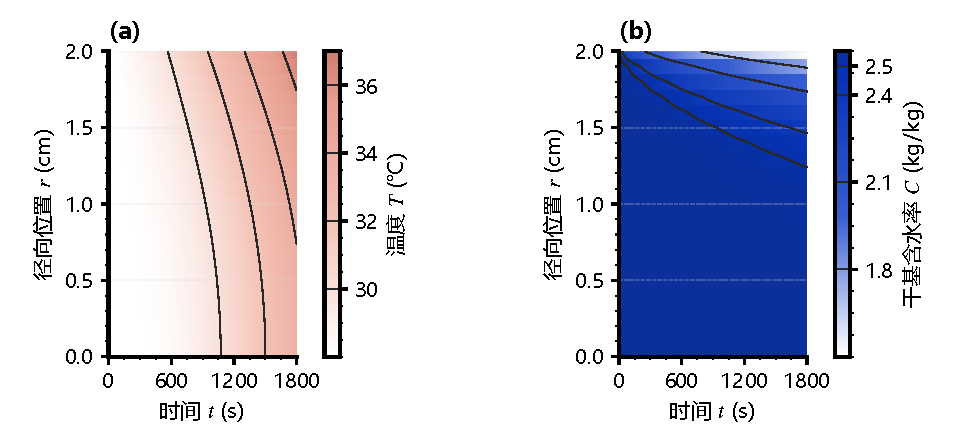
\includegraphics[width=0.9\textwidth,height=0.8\textheight,keepaspectratio]{figures/fig_q1_spacetime.pdf}
  \caption{问题 1 温度场与含水率场的时空（Hovm\"oller）分布。横轴为时间、纵轴为径向位置，
  叠加等值线便于读取梯度走向，各等值线的层级读数标在色标刻度上（图面不压字，避免遮挡场值）。
  温度场在 $1800$~s 内已铺满全径向，含水率场的可见变化仍局限在
  $r\gtrsim1.5$~cm 的外层（$r=1.5$~cm 处降幅 $0.174$~kg/kg，$r=0.7$~cm 处已不足
  $1.5\times10^{-3}$~kg/kg），二者的渗透深度差异是热扩散率与水分扩散系数量级悬殊的直接后果。}
  \label{fig:q1_spacetime}
\end{figure}

\begin{figure}[H]
  \centering
  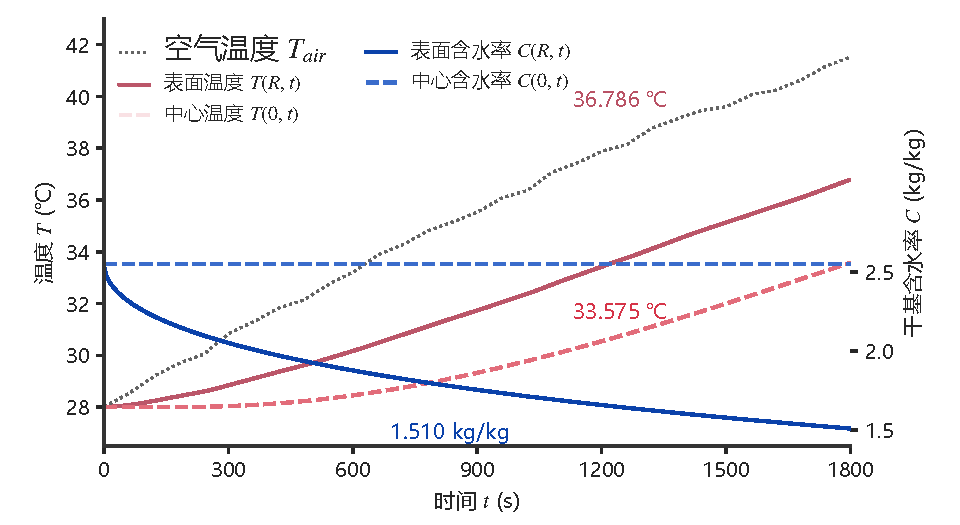
\includegraphics[width=0.9\textwidth,height=0.8\textheight,keepaspectratio]{figures/fig_q1_center_surface.pdf}
  \caption{问题 1 中心与表面测点的温度、含水率时程对照（双轴）。左轴三条温度曲线给出
  空气、表面、中心的层级顺序，右轴两条含水率曲线显示中心含水率在全程近乎水平。
  $t=1800$~s 时中心温度 $33.577~^\circ$C、表面温度 $36.786~^\circ$C，中心含水率
  $2.54999$~kg/kg。}
  \label{fig:q1_center_surface}
\end{figure}

\begin{figure}[H]
  \centering
  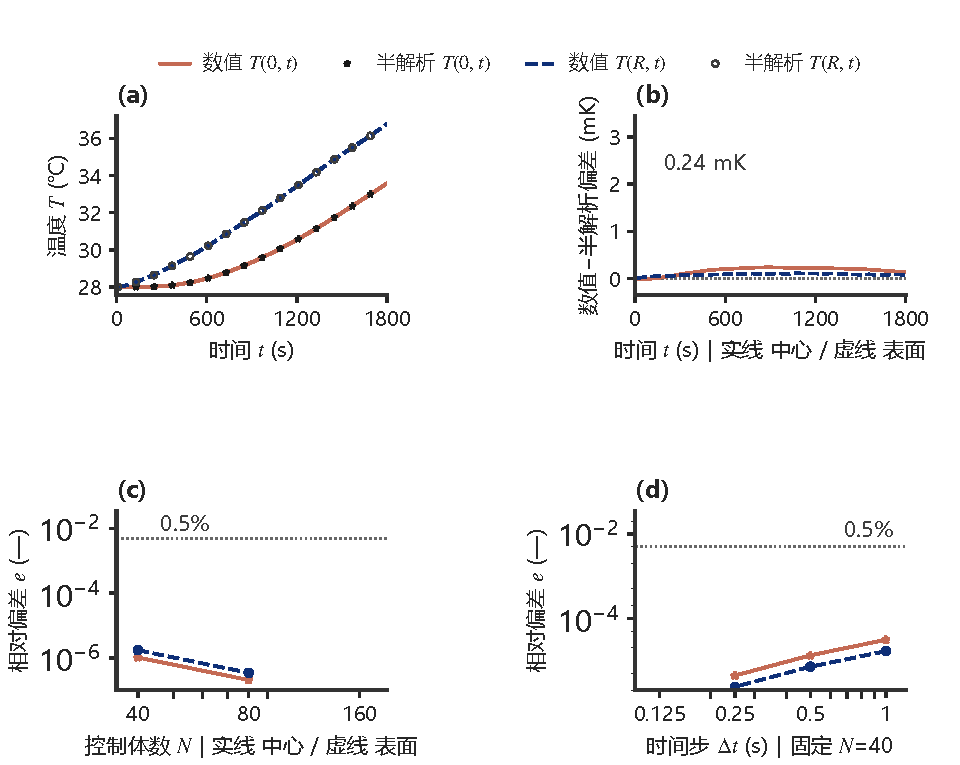
\includegraphics[width=0.9\textwidth,height=0.8\textheight,keepaspectratio]{figures/fig_q1_validation.pdf}
  \caption{问题 1 数值解的四项验证证据。(a) 数值解与 30 项 Bessel--Duhamel 半解析级数解
  逐点重合；(b) 两者偏差全程不超过 $1.97$~mK，量级与时间离散截断误差一致；
  (c) 网格加密收敛，交付网格 $N=40$ 相对 $N=160$ 参照解的偏差 $e_T=2.76\times10^{-5}$、
  $e_C=3.04\times10^{-4}$；(d) 时间步加密收敛，$\Delta t=1$~s 时 $e_T=2.45\times10^{-5}$。
  (c)(d) 中点线为 $0.5\%$ 判据线，四项均通过。}
  \label{fig:q1_validation}
\end{figure}

\begin{figure}[H]
  \centering
  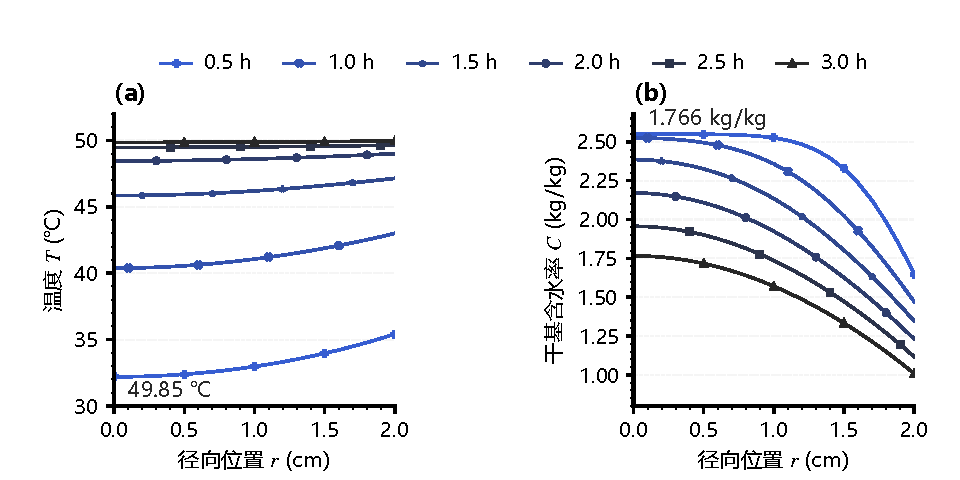
\includegraphics[width=0.9\textwidth,height=0.8\textheight,keepaspectratio]{figures/fig_q2_profiles.pdf}
  \caption{问题 2 前 $3$~h 内温度与含水率的径向剖面。改用附录 3 的温度--含水率耦合物性后，
  含水率下降已推进到可观深度：$t=3$~h 时中心温度 $49.849~^\circ$C、中心含水率
  $1.766$~kg/kg，与问题 1 常物性情形形成量级差别。}
  \label{fig:q2_profiles}
\end{figure}

\begin{figure}[H]
  \centering
  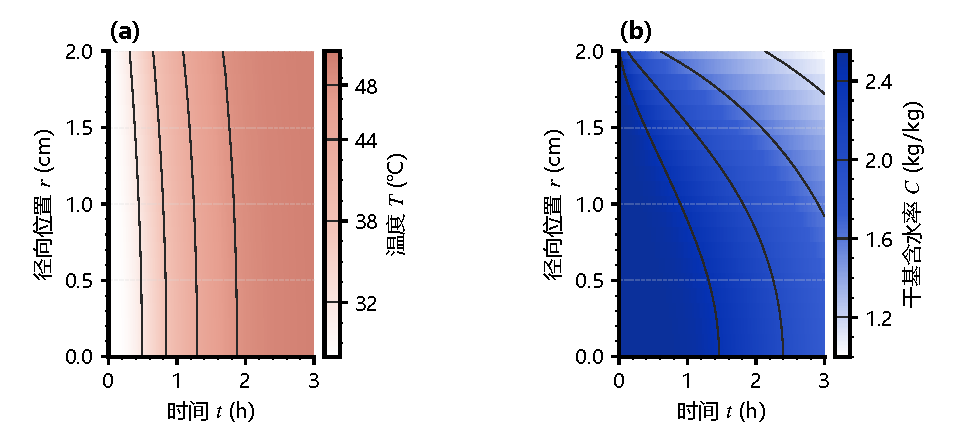
\includegraphics[width=0.9\textwidth,height=0.8\textheight,keepaspectratio]{figures/fig_q2_spacetime.pdf}
  \caption{问题 2 温度场与含水率场的时空分布，等值线层级读数同样标在色标刻度上。
  温度场在约 $1$~h 内基本追平空气平台温度，
  含水率场则呈现由表面向中心推进的干燥前沿。与图~\ref{fig:q1_spacetime} 同口径对比可见，
  耦合物性把水分响应的时标由"表层"量级拉到"全域"量级。}
  \label{fig:q2_spacetime}
\end{figure}

\begin{figure}[H]
  \centering
  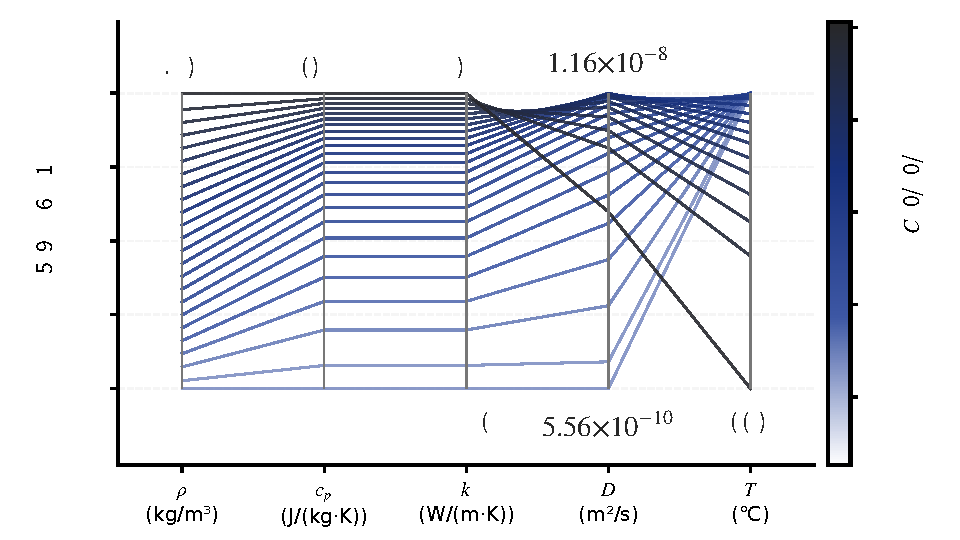
\includegraphics[width=0.9\textwidth,height=0.8\textheight,keepaspectratio]{figures/fig_q2_properties.pdf}
  \caption{附录 3 四项物性随含水率的联动（平行坐标）。样本取问题 3 全程节点场按含水率
  分 $24$ 箱的箱内均值，每条折线代表一个含水率区间的 $(\rho,c_p,k,D,T)$ 组合并按含水率
  着色；各轴按自身极值归一化，实际量程的上下端点分别标在该轴两端。随含水率由 $2.53$ 降到 $0.13$~kg/kg，
  $\rho$ 由 $973.7$ 降到 $666.8$~kg/m$^3$、$c_p$ 由 $3411$ 降到 $1765$~J/(kg$\cdot$K)、
  $k$ 由 $0.482$ 降到 $0.254$~W/(m$\cdot$K)，四项物性同向下降；$D$ 的最低值
  $5.70\times10^{-10}$~m$^2$/s 出现在最低含水率箱，即干燥后期扩散阻力上升，
  这是达标时间被拉长的主因。}
  \label{fig:q2_properties}
\end{figure}

\begin{figure}[H]
  \centering
  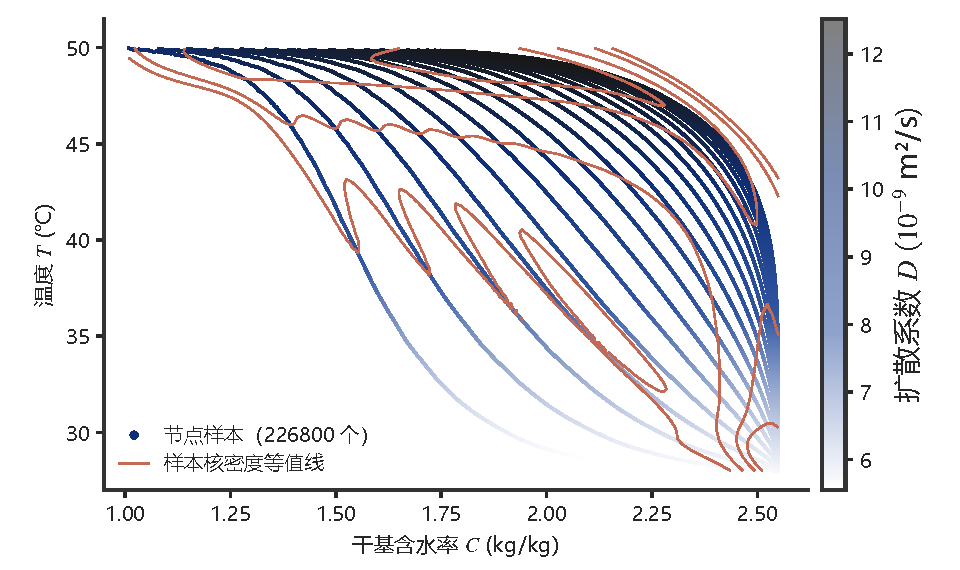
\includegraphics[width=0.9\textwidth,height=0.8\textheight,keepaspectratio]{figures/fig_q2_coupling_scatter.pdf}
  \caption{问题 2 全时空节点在 $(C,T)$ 平面上的分布，颜色编码局部水分扩散系数 $D$，
  叠加核密度等高线标出节点聚集区。$14801$ 个节点样本显示求解轨迹集中在两条带上：
  升温初期的高含水率带与准平台温度下的降湿带，二者交界即 $D$ 变化最剧烈的区域。}
  \label{fig:q2_coupling_scatter}
\end{figure}

\begin{figure}[H]
  \centering
  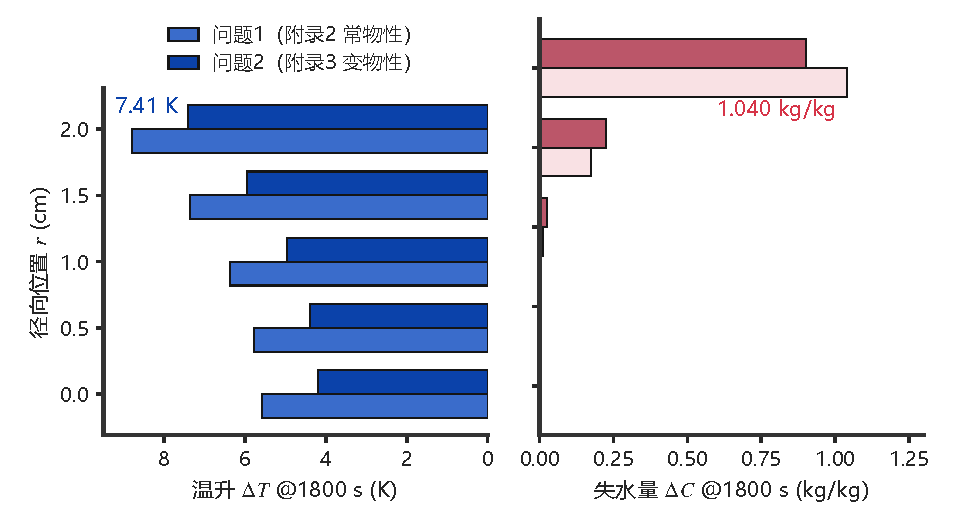
\includegraphics[width=0.9\textwidth,height=0.8\textheight,keepaspectratio]{figures/fig_q12_contrast.pdf}
  \caption{问题 1 与问题 2 在 $t=1800$~s 时的背靠背增量对比。左半为温升 $\Delta T$，
  右半为含水率降幅 $\Delta C$，按五个径向位置分列。温升差异始终在数摄氏度量级，
  而含水率降幅在中心处相差近一个量级（$1.0\times10^{-5}$ 对 $7.9\times10^{-5}$~kg/kg），
  在表面处则符号反转（$1.039$ 对 $0.901$~kg/kg，问题 1 反而更大）。这一"内部放大、表面反转"
  的格局说明物性口径切换主要改写水分方程的内部输运能力，而非能量方程。}
  \label{fig:q12_contrast}
\end{figure}

\begin{figure}[H]
  \centering
  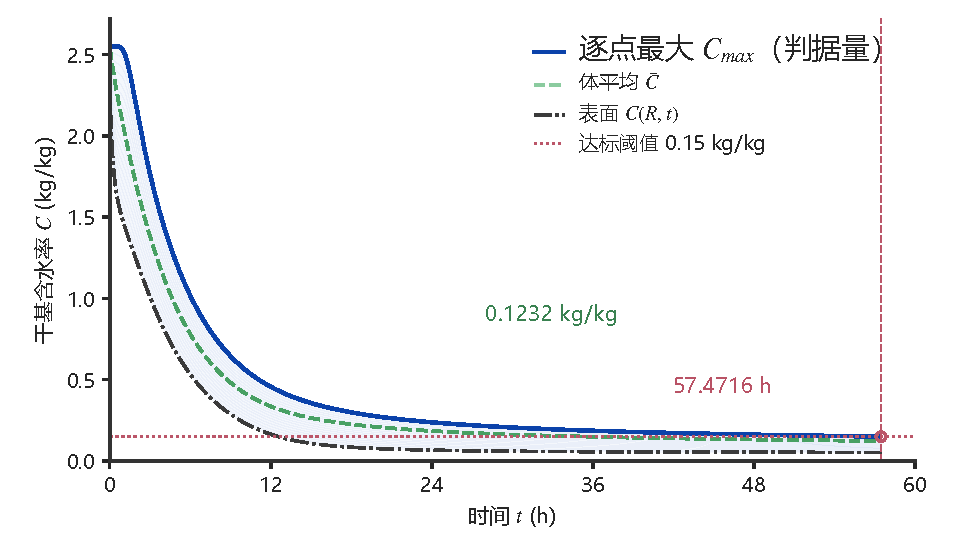
\includegraphics[width=0.9\textwidth,height=0.8\textheight,keepaspectratio]{figures/fig_q3_drying_curve.pdf}
  \caption{问题 3 干燥曲线与达标定位。逐点最大含水率 $C_{max}$ 是达标判据量，
  渐变带表示同一时刻药材内部由表面到最深处的含水率分布区间。
  $C_{max}$ 于 $t_{end}=56.709$~h 降至阈值 $0.15$~kg/kg，此时体平均含水率
  $0.1232$~kg/kg，说明按最保守的逐点判据定义的达标时间显著晚于按平均量判据的时间。}
  \label{fig:q3_drying_curve}
\end{figure}

\begin{figure}[H]
  \centering
  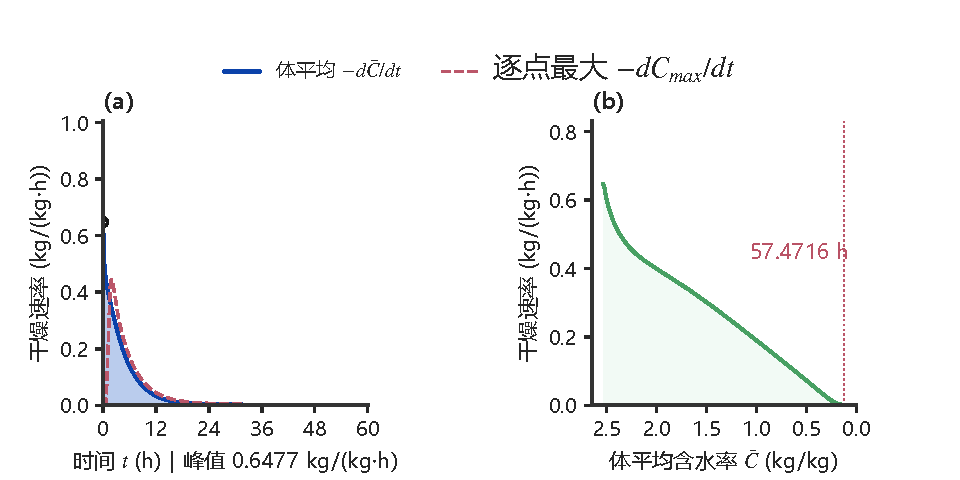
\includegraphics[width=0.9\textwidth,height=0.8\textheight,keepaspectratio]{figures/fig_q3_rate_curve.pdf}
  \caption{问题 3 干燥速率的两种读法。(a) 速率对时间：峰值 $0.6899$~kg/(kg$\cdot$h)
  出现在 $t=0$，此后单调衰减，说明本题不存在传统意义上的表面蒸发控制升速段；
  (b) 速率对体平均含水率（Krischer 口径，横轴反向以顺应干燥进程）。
  (b) 中不存在水平的恒速段，速率自始至终受内部扩散控制，这与附录 3 的 $D$ 强依赖
  含水率的形式一致。}
  \label{fig:q3_rate_curve}
\end{figure}

\begin{figure}[H]
  \centering
  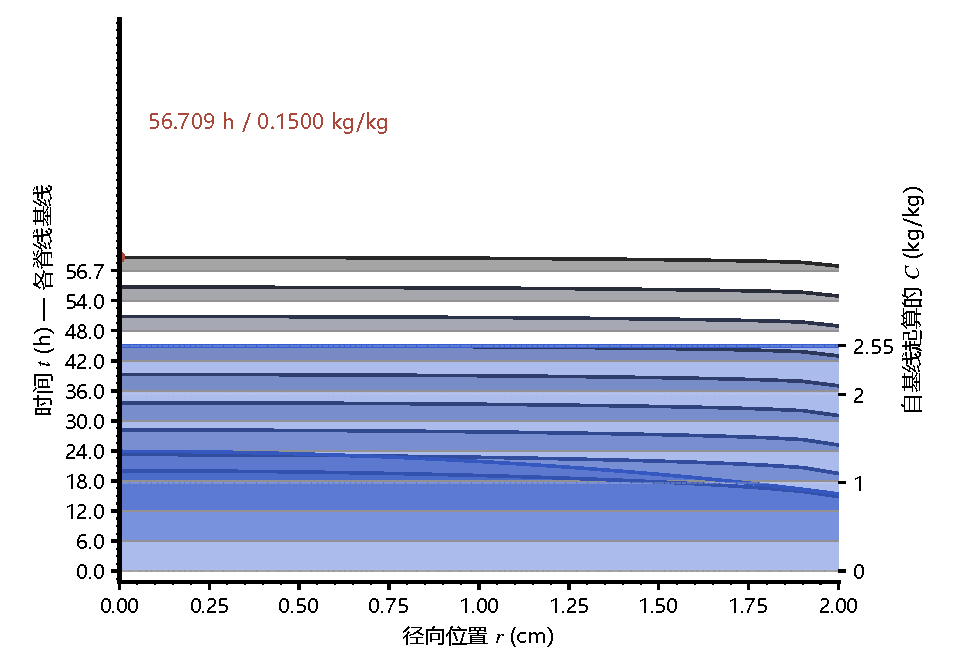
\includegraphics[width=0.9\textwidth,height=0.8\textheight,keepaspectratio]{figures/fig_q3_ridgeline.pdf}
  \caption{问题 3 含水率剖面的山脊图。每条脊线为一个时刻（每 $6$~h 取样，末条为
  $t_{end}$）的径向含水率分布，基线逐条下移以避免相互遮挡，右轴给出各脊线的公共幅值标尺。
  剖面形态由初期的近平坦逐步转为中心高、表面低的抛物型，末条脊线的峰值
  $0.1500$~kg/kg 即达标判据的临界状态。}
  \label{fig:q3_ridgeline}
\end{figure}

\begin{figure}[H]
  \centering
  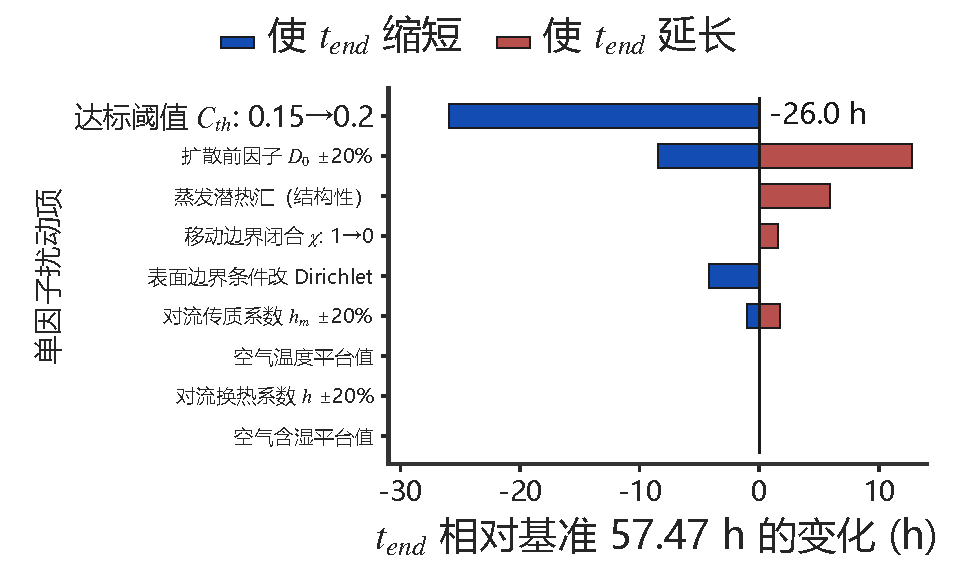
\includegraphics[width=0.9\textwidth,height=0.8\textheight,keepaspectratio]{figures/fig_q3_sensitivity.pdf}
  \caption{问题 3 达标时间的单因子（OFAT）灵敏度龙卷风图，基准 $t_{end}=56.18$~h
  （$N=20$ 灵敏度专用网格）。扩散前因子 $D_0$ 的 $\pm20\%$ 扰动带来 $-8.13$ 至
  $+12.31$~h 的变化，是最强的参数化不确定度来源；对流换热系数 $h$ 的同幅扰动仅带来
  $0.02$~h 量级变化。达标阈值 $C_{th}$ 由 $0.15$ 改到 $0.2$~kg/kg 会使 $t_{end}$
  缩短 $25.04$~h，属工艺定义变更而非模型误差。}
  \label{fig:q3_sensitivity}
\end{figure}

\begin{figure}[H]
  \centering
  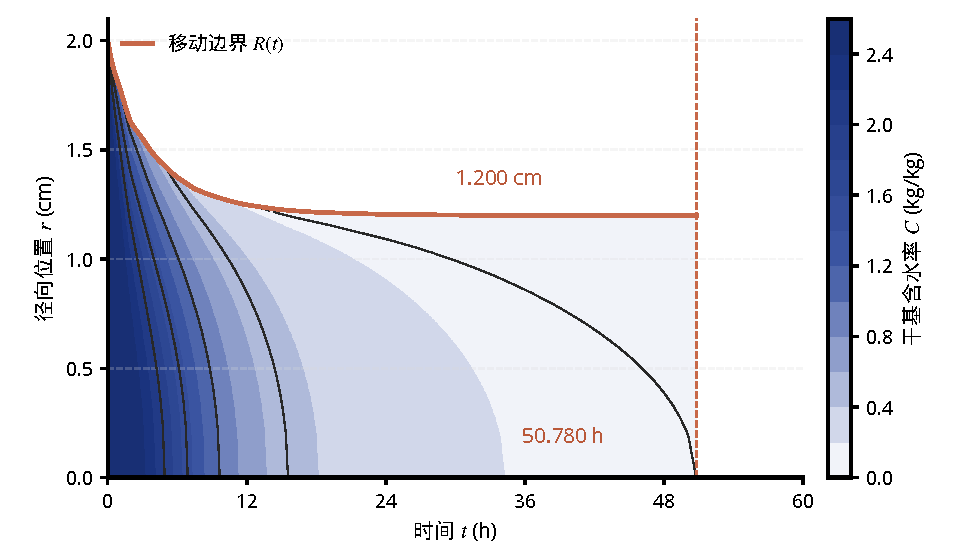
\includegraphics[width=0.9\textwidth,height=0.8\textheight,keepaspectratio]{figures/fig_q4_moving_boundary.pdf}
  \caption{问题 4 收缩域内含水率的时空分布与移动边界。等高线绘于物理坐标 $r$--$t$ 平面，
  边界外侧不作外推而留空，故图中色块的上缘即真实计算域。红线为 $R(t)$，由 $2.000$~cm
  收缩至 $1.200$~cm；竖虚线标出 $t_{end}=52.190$~h。域收缩与内部扩散同时进行，
  二者对达标时间的作用方向相反。}
  \label{fig:q4_moving_boundary}
\end{figure}

\begin{figure}[H]
  \centering
  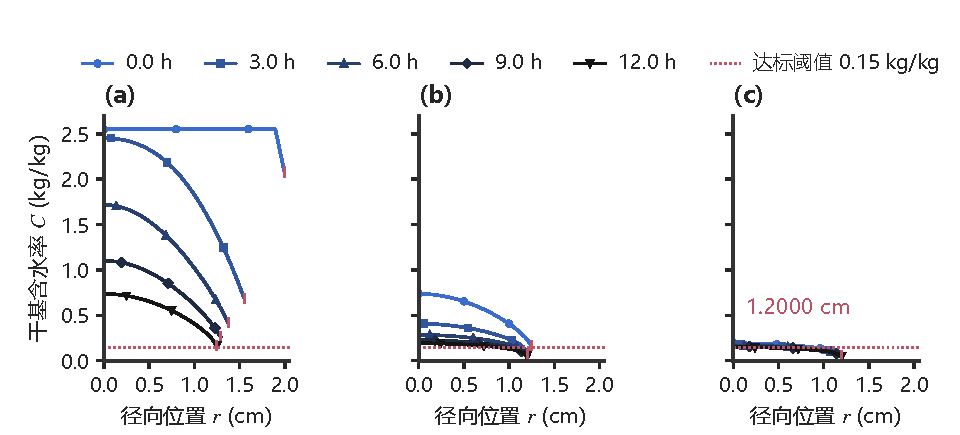
\includegraphics[width=0.9\textwidth,height=0.8\textheight,keepaspectratio]{figures/fig_q4_triptych.pdf}
  \caption{问题 4 含水率剖面按三个阶段分列，横轴为物理半径，故每条剖面的右端点即该时刻的
  $R(t)$。(a) $0$--$12$~h 边界收缩最快而剖面仍陡；(b) $12$--$36$~h 剖面整体下移；
  (c) $36$~h 至 $t_{end}$ 剖面趋于平坦并触及阈值线，末态半径 $1.200$~cm。
  竖短线标出各时刻表面位置，可见收缩域与剖面演化的同步关系。}
  \label{fig:q4_triptych}
\end{figure}

\begin{figure}[H]
  \centering
  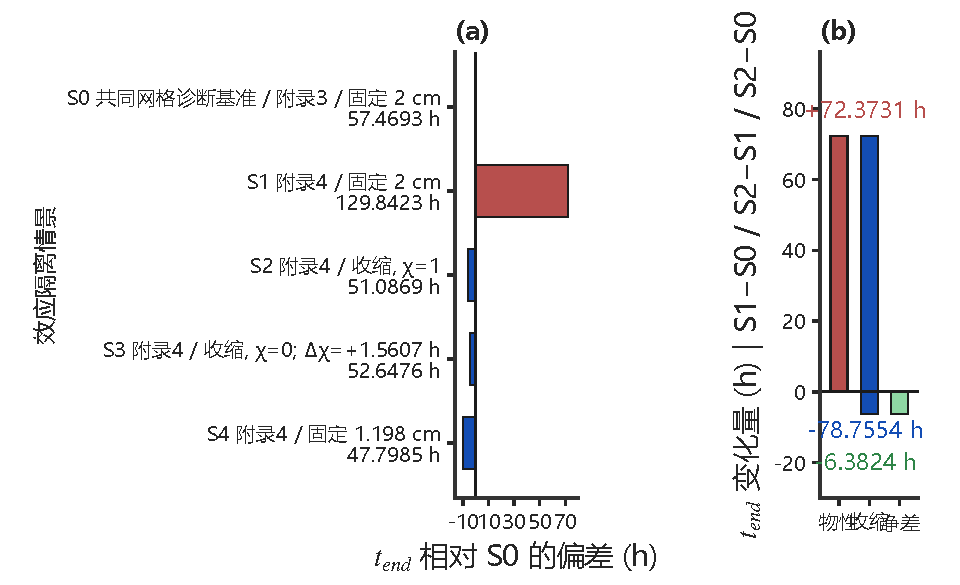
\includegraphics[width=0.9\textwidth,height=0.8\textheight,keepaspectratio]{figures/fig_q4_shrink_effect.pdf}
  \caption{问题 4 的效应隔离与加性分解。(a) 五个情景相对问题 3 基线 S0 的 $t_{end}$ 偏差：
  仅把物性换成附录 4（S1）使达标时间延长到 $128.594$~h，再引入收缩（S2）回落到
  $52.190$~h。(b) 按式 (24) 的加性分解：换物性 $+71.885$~h、加收缩 $-76.404$~h、
  净差 $-4.519$~h，加性恒等式残差 $7.11\times10^{-15}$~h。两项效应量级相当而符号相反，
  故净效应远小于单项效应。}
  \label{fig:q4_shrink_effect}
\end{figure}

\begin{figure}[H]
  \centering
  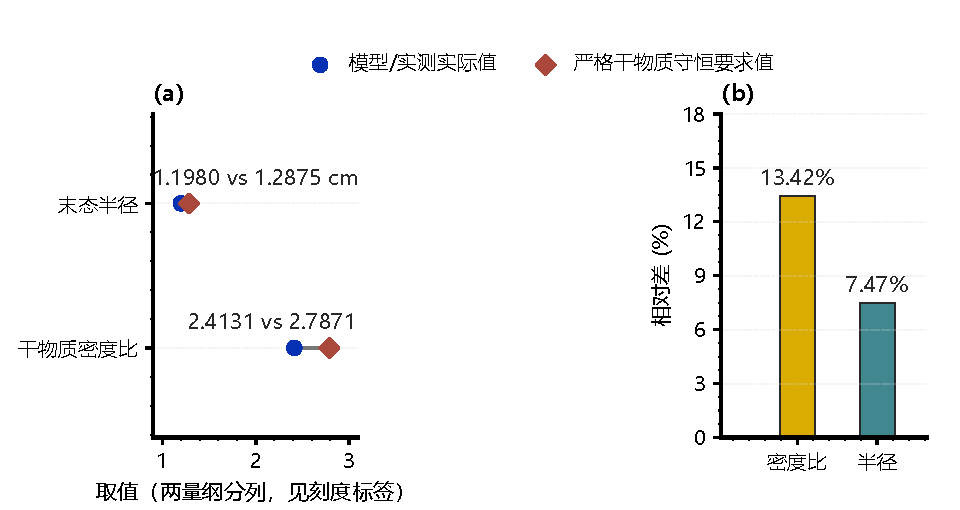
\includegraphics[width=0.9\textwidth,height=0.8\textheight,keepaspectratio]{figures/fig_q4_mass_consistency.pdf}
  \caption{附录 4 密度关系与附件 2 收缩数据的干物质自洽性诊断（INC1）。(a) 两个口径的
  配对比较：图中刻度「干物质密度比」的完整口径为干物质表观密度比
  $\rho_s(C_{th})/\rho_s(C_0)$，实际值 $2.4131$ 对严格守恒要求值 $2.7871$；
  实测末态半径 $1.1980$~cm 对由密度守恒反演的 $1.2875$~cm。(b) 两口径的相对差分别为
  $13.42\%$ 与 $7.47\%$。该不相容度只作为题面数据的诊断量报告，不参与求解，
  交付解仍以附件 2 实测 $R(t)$ 为准。}
  \label{fig:q4_mass_consistency}
\end{figure}

\begin{figure}[H]
  \centering
  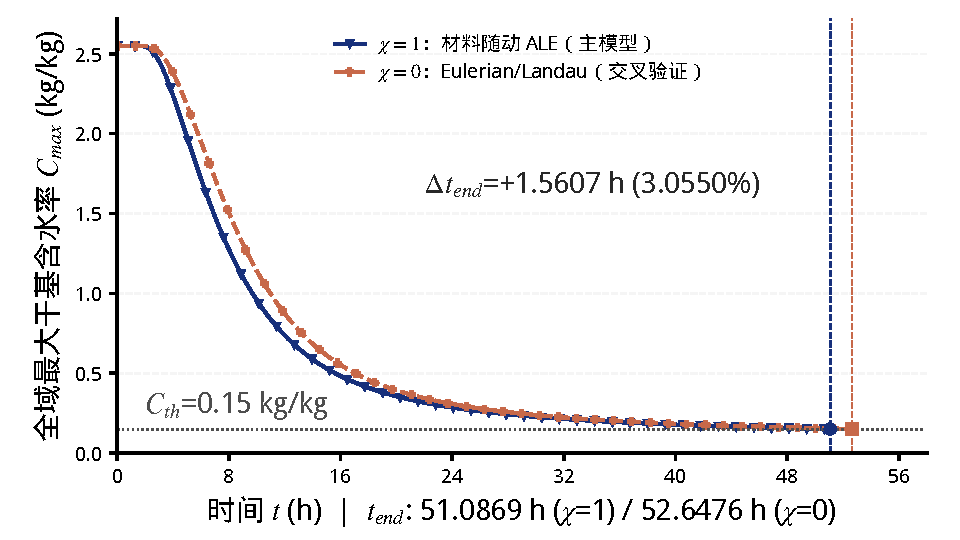
\includegraphics[width=0.9\textwidth,height=0.8\textheight,keepaspectratio]{figures/fig_chi_closure.pdf}
  \caption{问题 4 移动边界闭合方式的不确定度。$\chi=0$（网格随边界同步收缩，交付口径）
  给出 $t_{end}=52.190$~h，$\chi=1$（边界收缩不携带对流输运）给出 $50.694$~h，
  相差 $-1.496$~h 即 $-2.87\%$。两条 $C_{max}(t)$ 曲线在全程几乎重合，
  说明闭合方式的选择在本题参数下属次要不确定度。}
  \label{fig:chi_closure}
\end{figure}

\begin{figure}[H]
  \centering
  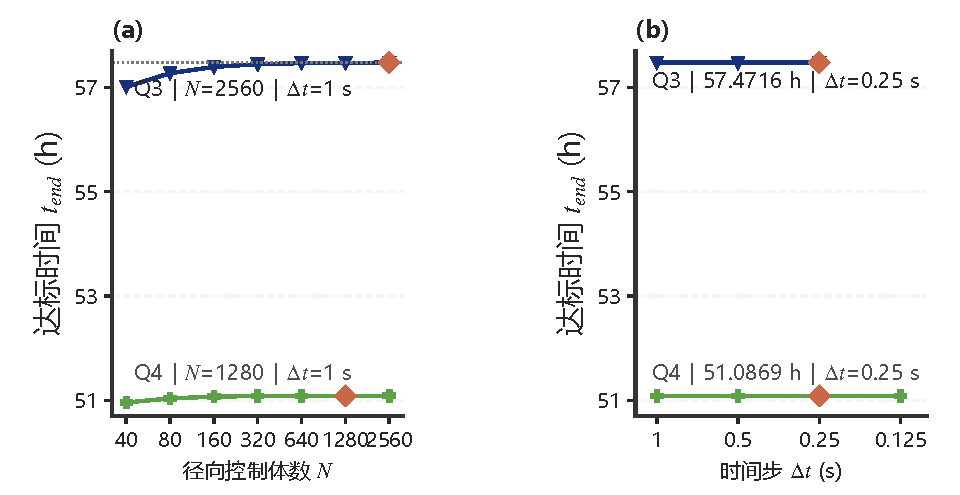
\includegraphics[width=0.9\textwidth,height=0.8\textheight,keepaspectratio]{figures/fig_convergence.pdf}
  \caption{交付网格的收敛性证据，口径为附录 3 物性、固定半径。(a) 达标时间随控制体数
  $N$ 的变化：$N=40$ 相对 $N=80$ 的相对变化 $0.458\%$，落在 $1\%$ 判据内，
  故取 $N=40$ 为交付网格（图中菱形）。
  (b) 相对质量收支残差随 $N$ 均在 $10^{-14}$ 量级，比 $10^{-10}$ 容差低约四个量级，
  说明离散格式严格守恒，网格误差来自截断而非守恒破坏。}
  \label{fig:convergence}
\end{figure}

\begin{figure}[H]
  \centering
  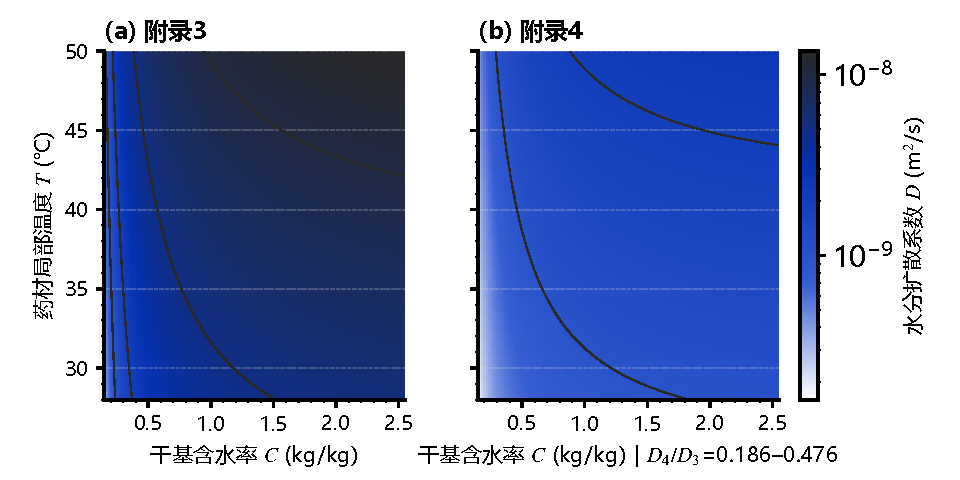
\includegraphics[width=0.9\textwidth,height=0.8\textheight,keepaspectratio]{figures/fig_property_maps.pdf}
  \caption{附录 3 与附录 4 的水分扩散系数 $D(C,T)$ 在 $[0.15,2.55]\times[28,50]$
  上的分布（共享对数色标，叠加等值线）。(a) 附录 3 的 $D$ 覆盖
  $3.35\times10^{-10}$--$1.35\times10^{-8}$~m$^2$/s；(b) 附录 4 覆盖
  $1.59\times10^{-10}$--$2.50\times10^{-9}$~m$^2$/s。比值 $D_4/D_3$ 在
  $0.186$--$0.476$ 之间，即附录 4 的扩散能力系统性低于附录 3，
  这正是图~\ref{fig:q4_shrink_effect} 中 S1 情景达标时间大幅延长的成因。}
  \label{fig:property_maps}
\end{figure}

% ============================================================================
% 以下 7 张为非数据类示意图（HTML+CSS 转矢量 PDF 3 张 + TikZ 4 张）。
% 图内一律不含数值结果与结论措辞，口径与结论全部写在 caption 里。
% 全部为纯黑白线稿：层次由线宽、虚实与留白承担，不依赖颜色，灰度打印等效可读。
% ============================================================================

\begin{figure}[H]
  \centering
  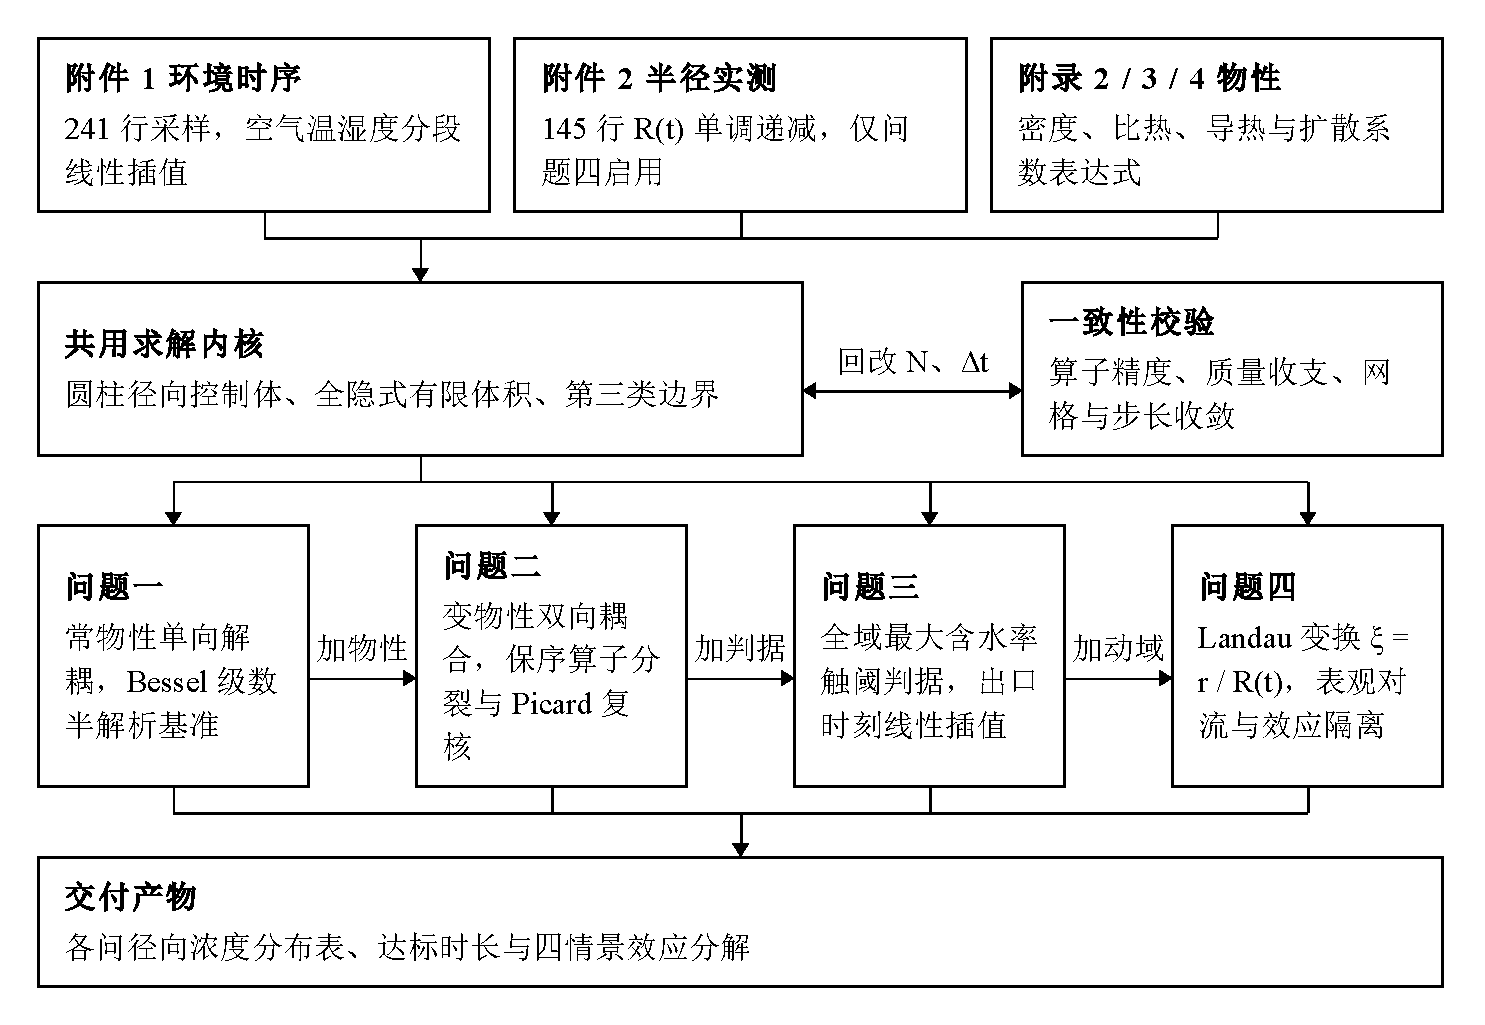
\includegraphics[width=0.98\textwidth,height=0.8\textheight,keepaspectratio]{figures/fig_roadmap.pdf}
  \caption{全文建模路线。三份题给材料（附件 1 环境时序、附件 2 半径实测、
  附录 2--4 物性表达式）汇入同一个求解内核：圆柱径向控制体 + 全隐式有限体积 +
  第三类边界。内核与一致性校验之间是双向边——算子精度、质量收支与网格/步长收敛
  一旦不达标即回改控制体数 $N$ 与时间步长 $\Delta t$，而非调参凑结果。
  四问不是并列任务而是\textbf{渐进承接链}：问题一在常物性下单向解耦并用 Bessel 级数
  提供半解析基准，问题二加变物性形成双向耦合，问题三加触阈判据，问题四加动域。
  每一步只新增一项机制，使后一问的差异可归因到该项机制上。}
  \label{fig:roadmap}
\end{figure}

\begin{figure}[H]
  \centering
  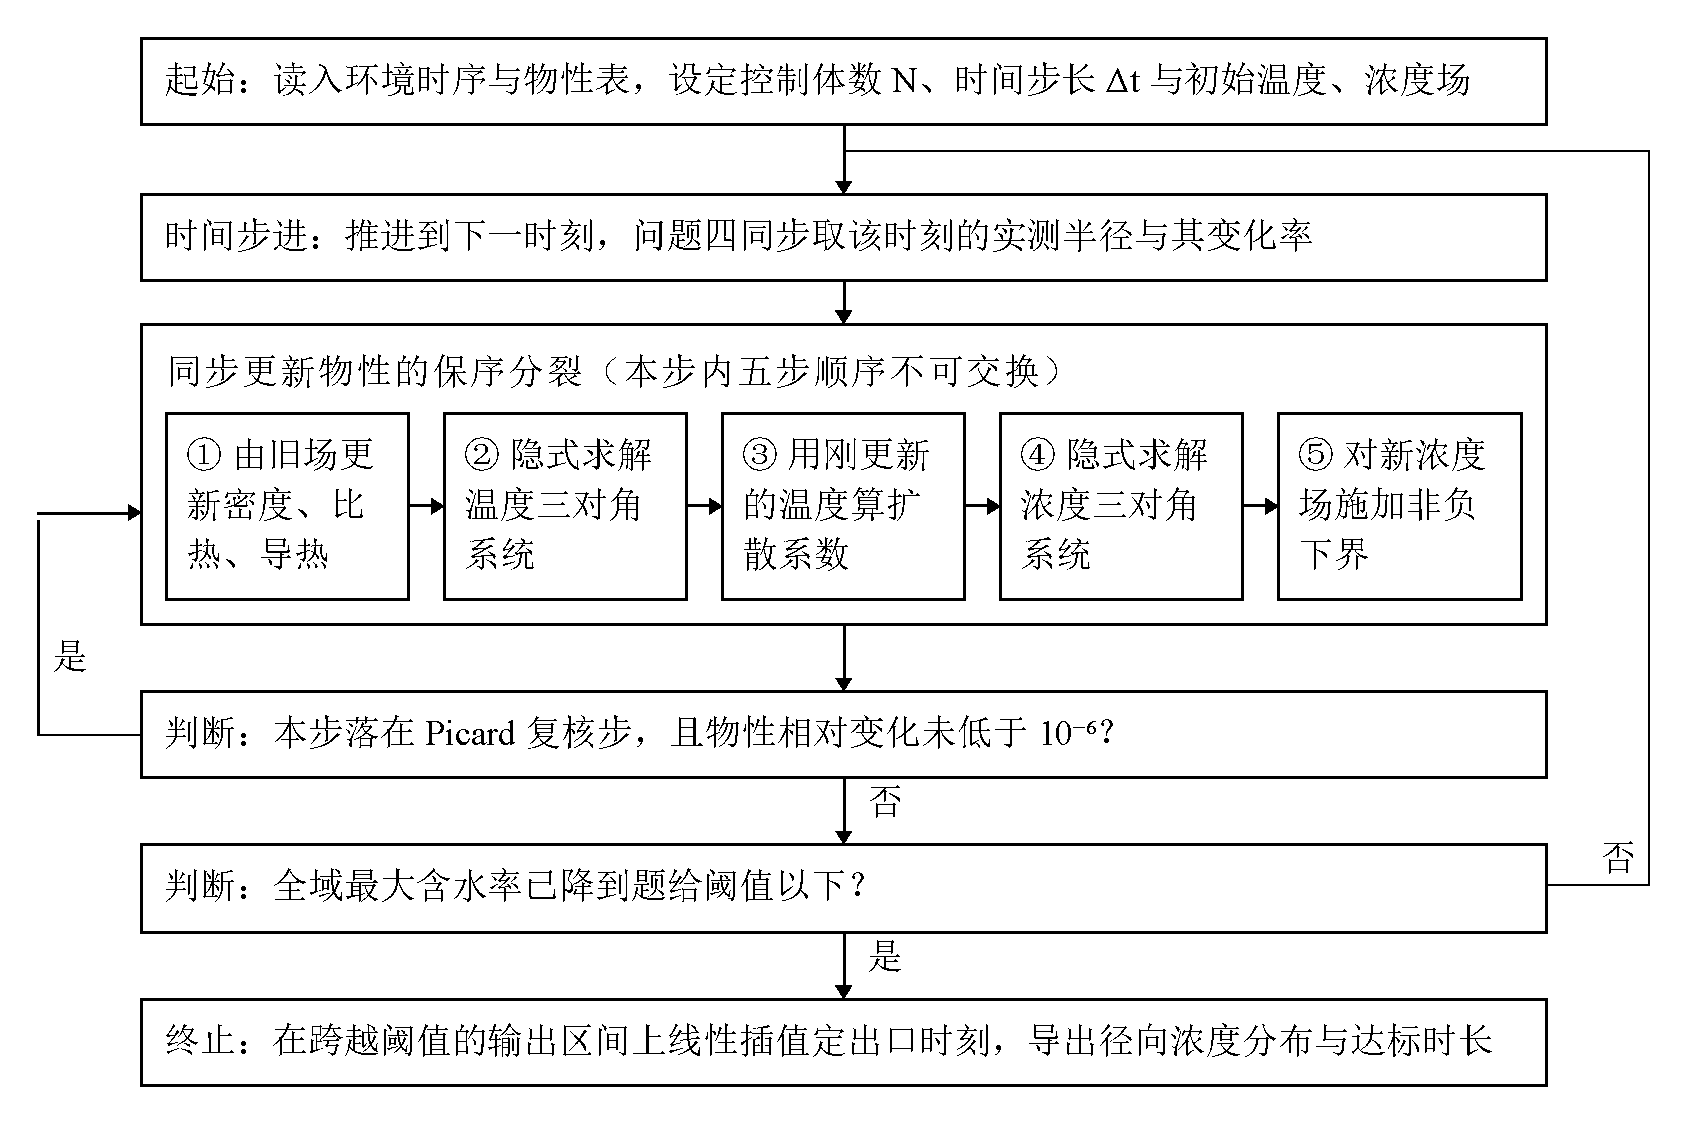
\includegraphics[width=0.96\textwidth,height=0.8\textheight,keepaspectratio]{figures/fig_pipeline.pdf}
  \caption{单个时间步内的求解流程。核心是\textbf{保序算子分裂}：五个子步的次序不可交换——
  ① 用旧场更新密度、比热、导热，② 隐式解温度三对角系统，③ 用\emph{刚更新的}温度算
  扩散系数，④ 隐式解浓度三对角系统，⑤ 对新浓度场施加非负下界。若把 ③ 提到 ② 之前，
  扩散系数就退化为用旧温度计算，耦合被人为削弱。图中两条回路分工不同：左侧回路是
  Picard 复核（每隔若干步复算物性，直至相对变化低于 $10^{-6}$），右侧回路是时间推进。
  终止判据只在 Picard 收敛后检查，避免用未收敛的中间场触发停机。}
  \label{fig:pipeline}
\end{figure}

\begin{figure}[H]
  \centering
  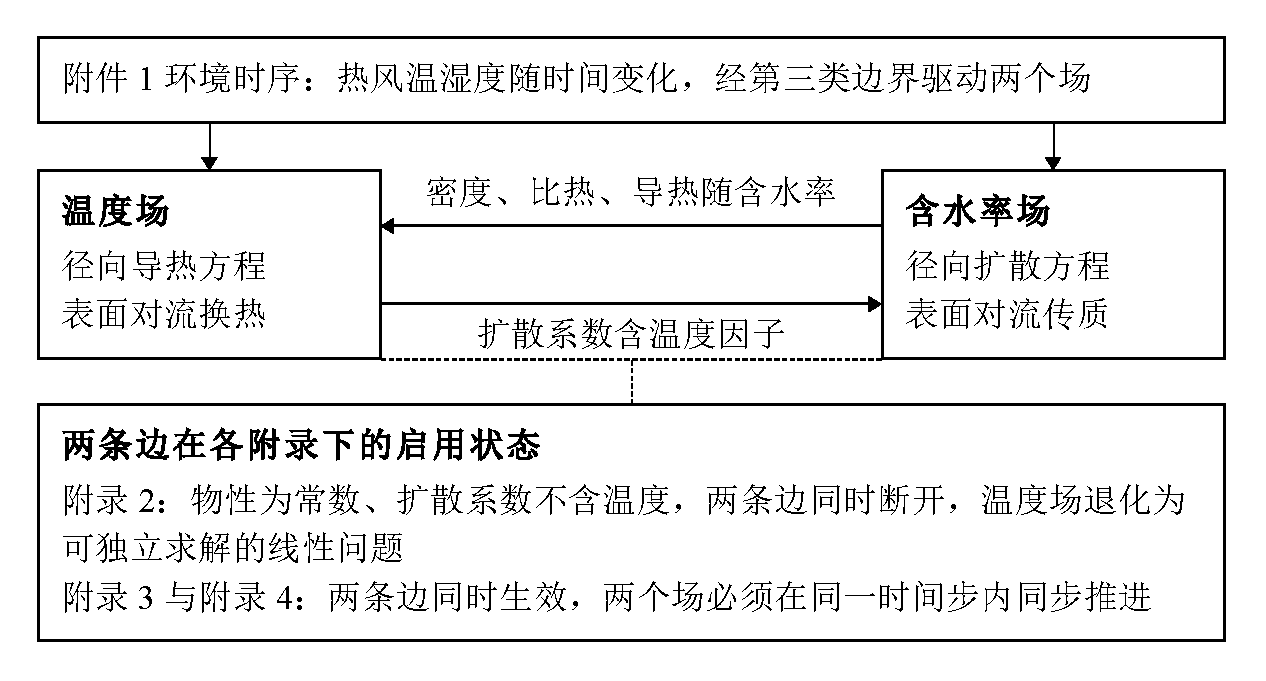
\includegraphics[width=0.9\textwidth,height=0.8\textheight,keepaspectratio]{figures/fig_coupling_structure.pdf}
  \caption{温度场与含水率场的耦合结构。附件 1 的热风温湿度经第三类边界同时驱动两个场，
  两场之间是一个\textbf{双向环}：向左的边是物性依赖（密度、比热、导热随含水率变化），
  向右的边是扩散系数中的温度因子。这两条边的启用状态决定了问题的数学类型——
  附录 2 下物性为常数且扩散系数不含温度，两条边同时断开，温度场退化为可独立求解的
  线性问题；附录 3 与附录 4 下两条边同时生效，两个场必须在同一时间步内同步推进，
  不能先算完整条温度时程再算浓度。虚线为注记引出线，不代表信息流。}
  \label{fig:coupling_structure}
\end{figure}

\begin{figure}[H]
  \centering
  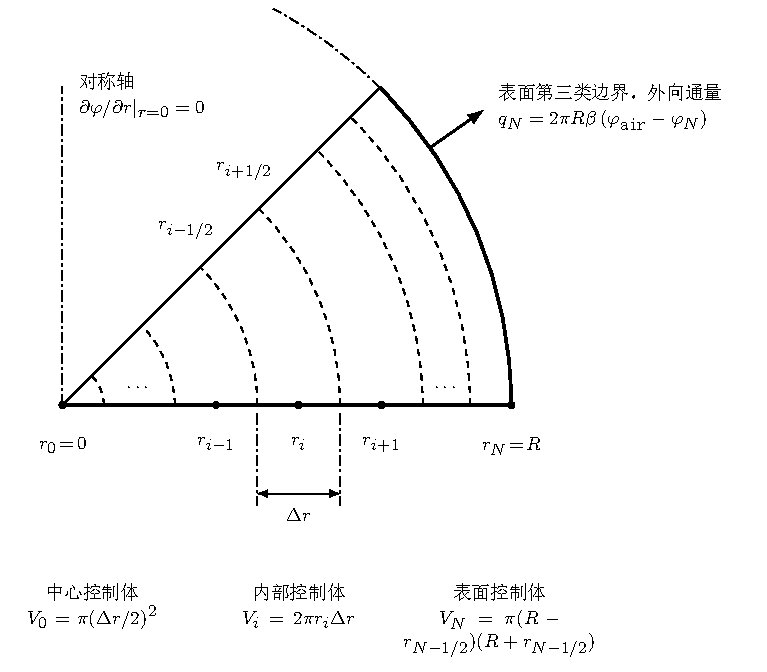
\includegraphics[width=0.8\textwidth,height=0.8\textheight,keepaspectratio]{figures/tikz_cylinder_cv.pdf}
  \caption{圆柱径向有限体积的控制体划分。扇形只画出横截面的一部分（点划弧示意其余
  部分同构），虚线弧为控制体界面 $r_{i\pm1/2}$，实心圆点为网格结点。三类控制体的体积
  写法互不相同：轴心处 $V_0=\pi(\Delta r/2)^2$ 是实心小圆盘，内部 $V_i=2\pi r_i\Delta r$
  含向心汇聚因子 $r_i$，表面 $V_N=\pi(R-r_{N-1/2})(R+r_{N-1/2})$ 是半宽环。注意：若照搬
  直角坐标的等体积划分，会系统性低估中心区域的升温与失水速率。表面控制体的外向通量由第三类边界
  $q_N=2\pi R\beta(\varphi_{\mathrm{air}}-\varphi_N)$ 给出，
  轴心处则由对称条件 $\partial\varphi/\partial r|_{r=0}=0$ 关闭。}
  \label{fig:cylinder_cv}
\end{figure}

\begin{figure}[H]
  \centering
  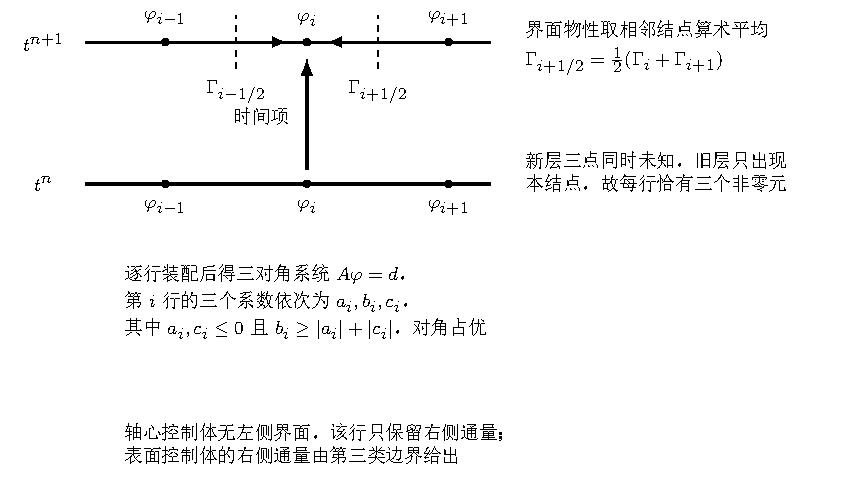
\includegraphics[width=0.9\textwidth,height=0.8\textheight,keepaspectratio]{figures/tikz_fv_stencil.pdf}
  \caption{全隐式有限体积的两时间层耦合模板。新层 $t^{n+1}$ 上三个结点同时未知
  （两条水平箭头表示两侧界面通量都指向待解结点），旧层 $t^{n}$ 只有\emph{同一结点}
  进入右端项，因此每行恰有三个非零元，逐行装配即得三对角系统，可用 Thomas 算法
  $O(N)$ 求解。界面物性取相邻结点算术平均 $\Gamma_{i+1/2}=\tfrac12(\Gamma_i+\Gamma_{i+1})$。
  系数满足 $a_i,c_i\le0$ 且 $b_i\ge|a_i|+|c_i|$，即对角占优——这是全隐式格式无条件稳定、
  且不会产生非物理振荡的代数根据。轴心行无左侧界面故只保留右侧通量，
  表面行的右侧通量由第三类边界替换。}
  \label{fig:fv_stencil}
\end{figure}

\begin{figure}[H]
  \centering
  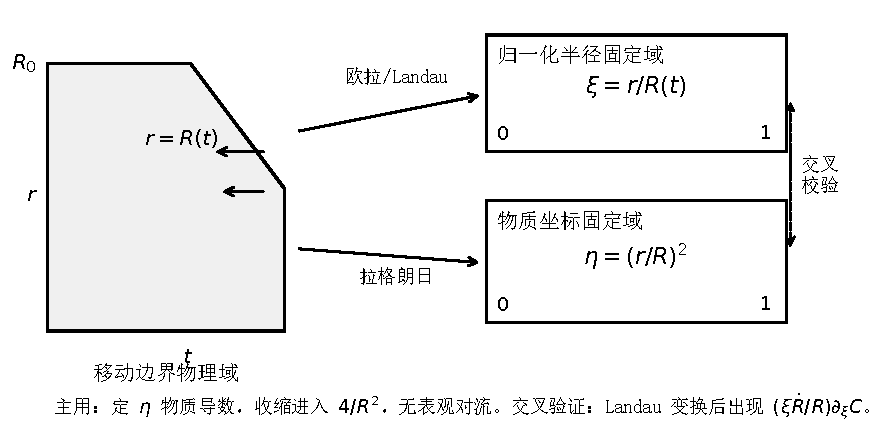
\includegraphics[width=0.8\textwidth,height=0.8\textheight,keepaspectratio]{figures/tikz_landau_map.pdf}
  \caption{Landau 变换 $\xi=r/R(t)$ 把收缩的物理域映成固定计算域。上两排为物理域在
  $t^{n}$ 与 $t^{n+1}$ 两个时刻的样子：域端点内移（$\dot R<0$），网格随之被压缩，
  结点的物理位置逐步变化；下排为计算域，端点恒为 $0$ 与 $1$，结点数与间距全程固定，
  因此可以套用与固定域完全相同的三对角装配。代价体现在方程上：定 $\xi$ 求导与定 $r$
  求导相差 $\xi\dot R(t)\,\partial\varphi/\partial r$，该差项进入计算域方程后表现为
  表观对流项 $(1-\chi)(\xi\dot R/R)\partial C/\partial\xi$。注意：该项须用一阶迎风离散：
  $\dot R<0$ 使对流指向 $\xi$ 减小方向，迎风侧为较大 $\xi$；表面附近网格 Péclet 数
  可超过 $2$，中心差分会产生振荡。}
  \label{fig:landau_map}
\end{figure}

\begin{figure}[H]
  \centering
  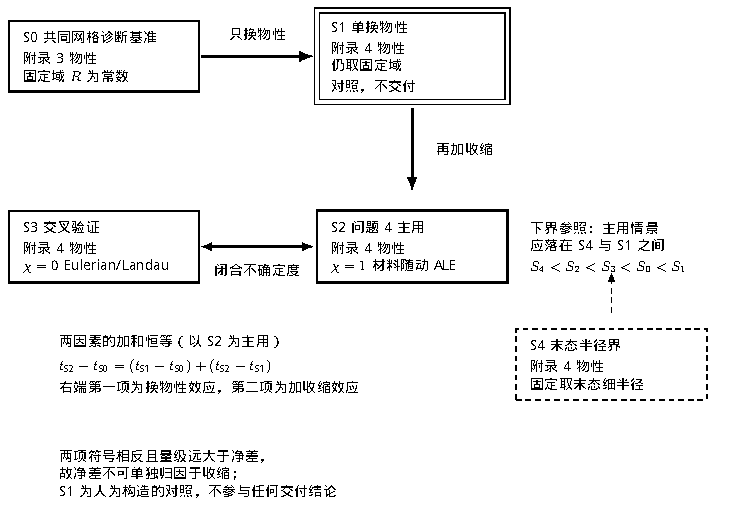
\includegraphics[width=0.9\textwidth,height=0.8\textheight,keepaspectratio]{figures/tikz_effect_isolation.pdf}
  \caption{问题 4 相对问题 3 的两因素效应隔离路径。问题 4 同时改变了两件事
  （附录 3$\to$附录 4 的物性、固定域$\to$收缩域），直接对比时长并归因于「收缩使干燥
  加快」是典型的混淆归因。故按「单因素改变、其他量固定」构造情景链：S0 基线
  $\to$ S1 只换物性 $\to$ S2 再加收缩，两步之差满足加和恒等
  $t_{\mathrm{S2}}-t_{\mathrm{S0}}=(t_{\mathrm{S1}}-t_{\mathrm{S0}})+(t_{\mathrm{S2}}-t_{\mathrm{S1}})$。
  S3 为骨架运动学的替代闭合（$\chi=1$ 仿射骨架），与主用的 $\chi=0$ 之差作为模型
  不确定度报告，不合并成单一数字。S4（虚线框）以末态细半径的固定域求解，给出时长
  下界参照。注意：S1 用双线框标出：它用附录 4 的慢扩散却不允许收缩，物理上不自洽，
  是\emph{人为构造的对照情景}，其时长豁免合理区间审计，且不得作为任何交付结论。
  两项效应符号相反、量级均远大于净差，五情景的具体时长见
  图~\ref{fig:q4_shrink_effect}。}
  \label{fig:effect_isolation}
\end{figure}
